\documentclass[12pt,a4paper]{report}
\usepackage[utf8]{inputenc}
\usepackage[T1]{fontenc}
\usepackage{amsmath, amssymb, amsthm}
\usepackage{geometry}
\usepackage{booktabs}
\usepackage{xcolor}
\usepackage{hyperref}
\usepackage{parskip}
\usepackage{fancyvrb}
\usepackage{listings}
\usepackage{graphicx}
\usepackage{float}
\usepackage{tikz}
\usepackage{amsmath}
\usepackage{amsthm}
\usepackage{enumitem}
\geometry{margin=2.5cm}

\hypersetup{
    colorlinks=true,
    linkcolor=blue!60!black,
    urlcolor=blue!60!black
}
\newtheorem{definition}{Definition}
\newtheorem{claim}{Claim}
\newtheorem{proposition}{Proposition}
\newtheorem{theorem}{Theorem}
\newtheorem{observation}{Observation}
\newtheorem{lemma}{Lemma}
\newtheorem{corollary}{Corollary}

\title{\textbf{Algorithm Design} \\ \large Notes}
\author{}
\date{}

\begin{document}

\maketitle
\tableofcontents

% ─────────────────────────────────────────────
\chapter{Algorithm Analysis}
\section{Computational Tractability}

The question of how to solve a problem in the \emph{shortest possible time} is not new.
A simple approach to many problems is \textbf{brute force}: try every possible solution and
pick the best one. The problem is that this usually takes \(2^n\) time or worse, where
\(n\) is the size of the input. For large inputs, this is completely impractical.

\subsection{Polynomial Running Time}

We say that an algorithm is \textbf{efficient} if its running time is \emph{polynomial}.
\newline
\begin{definition}[Polynomial-time algorithm]
An algorithm runs in polynomial time if there exist constants $c > 0$ and $d > 0$ such
that, on every input of size $n$, its running time is at most $c \cdot n^d$ steps.
\end{definition}

A useful way to think about this: if you \emph{double} the input size, the running time
should only grow by a constant factor $C = 2^d$.

(To represent the number x we need $\log_2 x$ bits, so the input size is $n = \log_2 x$. If the algorithm runs in polynomial time, then the running time is $O(n^d) = O((\log_2 x)^d) = O(\log_2^d x)$)

The input change for combinatorial problems and numerical problems is different. For combinatorial problems, the input size is typically the number of elements (e.g., nodes in a graph), while for numerical problems, the input size is the number of bits needed to represent the numbers.

\textbf{Why polynomial = efficient?} In practice, poly-time algorithms tend to have small
constants and small exponents. Also, breaking the exponential barrier usually means
discovering an important structure in the problem.

\textbf{Exceptions.} A few poly-time algorithms have very large constants and are not
useful in practice. On the other hand, some exponential-time algorithms (like the Simplex
method) are widely used because the worst cases almost never happen in real life.

\subsection{Types of Analysis}

There are several ways to measure the running time of an algorithm:

\begin{center}
\begin{tabular}{@{}lll@{}}
\toprule
\textbf{Type} & \textbf{Description} & \textbf{Example} \\
\midrule
Worst-case   & Guarantee for \emph{any} input of size $n$ & Heapsort: $\leq 2n\log_2 n$ compares \\
Probabilistic & Expected time of a randomised algorithm   & Quicksort: $\sim 2n\ln n$ compares \\
Amortised    & Worst-case over a sequence of $n$ operations & Stack resize: $O(n)$ for $n$ push/pop \\
Average-case & Expected time on a random input           & 3-way radix sort: $\sim 2n\ln n$ \\
\bottomrule
\end{tabular}
\end{center}

\textbf{Worst-case analysis} is the most common. It gives a solid guarantee for all
possible inputs and usually reflects real performance well.

Sometimes the algorithms aren't deterministic, so we use \textbf{probabilistic analysis} to measure the expected running time. This is common for randomised algorithms, which use random bits to make decisions.In this case, we use the expcted value of the running time over the random choices of the algorithm.
% ─────────────────────────────────────────────
\section{Asymptotic Order of Growth}

Asymptotic notation lets us describe how the running time \emph{grows} as $n$ gets large,
ignoring small constant factors.

\subsection{Big-O Notation (Upper Bound)}

\begin{definition}[Big-O]
$T(n)$ is $O(f(n))$ if there exist constants $c > 0$ and $n_0 \geq 0$ such that
\[
    T(n) \leq c \cdot f(n) \quad \text{for all } n \geq n_0.
\]
\end{definition}

\noindent
\begin{minipage}[t]{0.3\textwidth}
\vspace{0pt}
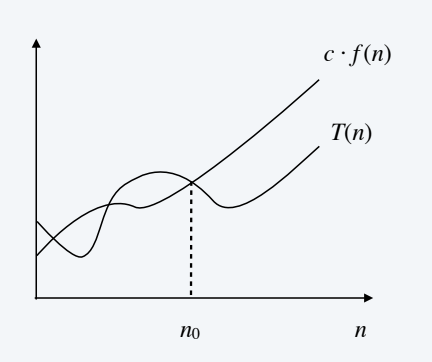
\includegraphics[width=\textwidth]{imm/O-grande.png}
\end{minipage}%
\hfill
\begin{minipage}[t]{0.65\textwidth}
\vspace{0pt}
An equivalent condition using limits:
\[
    \limsup_{n \to \infty} \frac{T(n)}{f(n)} < \infty.
\]

\textbf{Example.} Let $T(n) = 32n^2 + 17n + 1$. Then:
\begin{itemize}
    \item $T(n)$ is $O(n^2)$ \quad (choose $c = 50$, $n_0 = 1$)
    \item $T(n)$ is also $O(n^3)$
    \item $T(n)$ is \emph{not} $O(n)$ nor $O(n \log n)$
\end{itemize}
\end{minipage}

\textbf{Typical use.} ``Insertion sort makes $O(n^2)$ compares to sort $n$ elements.''

\textbf{Note on notation.} Technically, $O(f(n))$ is a \emph{set} of functions, but
computer scientists write $T(n) = O(f(n))$ as shorthand. This is an accepted abuse of
notation — just be careful not to misuse it (e.g., writing $O(n) = O(n^2)$ is fine, but
not the reverse).

\subsection{Big-Omega Notation (Lower Bound)}

\begin{definition}[Big-Omega]
$T(n)$ is $\Omega(f(n))$ if there exist constants $c > 0$ and $n_0 \geq 0$ such that
\[
    T(n) \geq c \cdot f(n) \quad \text{for all } n \geq n_0.
\]
\end{definition}

\textbf{Example.} For $T(n) = 32n^2 + 17n + 1$:
\begin{itemize}
    \item $T(n)$ is $\Omega(n^2)$ and $\Omega(n)$
    \item $T(n)$ is \emph{not} $\Omega(n^3)$
\end{itemize}

\textbf{Typical use.} ``Any comparison-based sorting algorithm requires $\Omega(n \log n)$
compares in the worst case.''

\medskip
\textbf{Common mistake.} It is meaningless to say ``requires \emph{at least} $O(n \log n)$
compares'' — Big-O is an upper bound, not a lower bound.

\subsection{Big-Theta Notation (Tight Bound)}

\begin{definition}[Big-Theta]
$T(n)$ is $\Theta(f(n))$ if there exist constants $c_1 > 0$, $c_2 > 0$, and $n_0 \geq 0$
such that
\[
    c_1 \cdot f(n) \leq T(n) \leq c_2 \cdot f(n) \quad \text{for all } n \geq n_0.
\]
\end{definition}

In other words, $T(n)$ is $\Theta(f(n))$ if and only if it is both $O(f(n))$ and
$\Omega(f(n))$.

\textbf{Example.} Mergesort makes $\Theta(n \log n)$ compares. For
$T(n) = 32n^2 + 17n + 1$: $T(n)$ is $\Theta(n^2)$, but not $\Theta(n)$ or $\Theta(n^3)$.

\subsection{Useful Limit Rules}

\begin{proposition}
If $\displaystyle\lim_{n \to \infty} \frac{f(n)}{g(n)} = c > 0$, then $f(n)$ is $\Theta(g(n))$.
\end{proposition}

\begin{proposition}
If $\displaystyle\lim_{n \to \infty} \frac{f(n)}{g(n)} = 0$, then $f(n)$ is $O(g(n))$ but not $\Omega(g(n))$.
\end{proposition}

\textbf{Proof sketch for the first proposition.} By definition of the limit, there exists
$n_0$ such that for all $n \geq n_0$:
\[
    \frac{c}{2} < \frac{f(n)}{g(n)} < 2c
    \quad \Rightarrow \quad
    \frac{c}{2} \cdot g(n) \leq f(n) \leq 2c \cdot g(n).
\]
This gives both the upper and lower bound needed for $\Theta$. \hfill$\square$

\subsection{Key Asymptotic Facts}

\begin{itemize}
    \item \textbf{Polynomials.} If $T(n) = a_0 + a_1 n + \cdots + a_d n^d$ with $a_d > 0$,
    then $T(n)$ is $\Theta(n^d)$, because
    \[
        \lim_{n \to \infty} \frac{a_0 + a_1 n + \cdots + a_d n^d}{n^d} = a_d > 0.
    \]

    \item \textbf{Logarithm base does not matter.} $\Theta(\log_a n) = \Theta(\log_b n)$
    for any constants $a, b > 0$ (by change-of-base formula). We simply write $\log n$.

    \item \textbf{Logs are slower than polynomials.} For every $d > 0$,
    $\log n$ is $O(n^d)$.

    \item \textbf{Polynomials are slower than exponentials.} For every $r > 1$ and $d > 0$,
    $n^d$ is $O(r^n)$, i.e.,
    \[
        \lim_{n \to \infty} \frac{n^d}{r^n} = 0.
    \]
\end{itemize}

\subsection{Big-O with Multiple Variables}

Sometimes the input has two parameters (e.g., nodes and edges in a graph).

\begin{definition}
$T(m, n)$ is $O(f(m, n))$ if there exist constants $c > 0$, $m_0 \geq 0$, $n_0 \geq 0$
such that $T(m,n) \leq c \cdot f(m,n)$ for all $n \geq n_0$ and $m \geq m_0$.
\end{definition}

\textbf{Example.} $T(m,n) = 32mn^2 + 17mn + 32n^3$ is $O(mn^2 + n^3)$ and also
$O(mn^3)$, but it is \emph{neither} $O(n^3)$ nor $O(mn^2)$.

\textbf{Typical use.} Breadth-first search (BFS) takes $O(m + n)$ time to find the
shortest path from $s$ to $t$ in a directed graph with $n$ nodes and $m$ edges.

% ─────────────────────────────────────────────
\section{Survey of Common Running Times}

The table below shows the most common complexity classes, from fastest to slowest.

\begin{center}
\begin{tabular}{@{}lll@{}}
\toprule
\textbf{Complexity} & \textbf{Name} & \textbf{Example} \\
\midrule
$O(\log n)$   & Sublinear / Logarithmic & Binary search \\
$O(n)$        & Linear                  & Finding max, merging two lists \\
$O(n \log n)$ & Linearithmic            & Mergesort, Heapsort \\
$O(n^2)$      & Quadratic               & Closest pair (naive) \\
$O(n^3)$      & Cubic                   & Set disjointness \\
$O(n^k)$      & Polynomial              & Independent set of size $k$ \\
$O(2^n)$      & Exponential             & Maximum independent set \\
\bottomrule
\end{tabular}
\end{center}

\subsection{Logarithmic Time — O(log n)}

The running time grows very slowly — doubling the input only adds one step.

\textbf{Binary search.} Given a sorted array $A$ of $n$ numbers, find whether $x$ is
in the array.

\begin{Verbatim}[frame=single]
lo = 1, hi = n
while (lo <= hi):
    mid = (lo + hi) / 2
    if   x < A[mid]: hi = mid - 1
    elif x > A[mid]: lo = mid + 1
    else: return YES
return NO
\end{Verbatim}

Each iteration cuts the search interval in half, so at most $\lceil \log_2 n \rceil$
iterations are needed.

\subsection{Linear Time — O(n)}

The running time grows proportionally to the input size.

\textbf{Example 1 — Maximum of $n$ numbers.}
\begin{Verbatim}[frame=single]
max = a[1]
for i = 2 to n:
    if a[i] > max:
        max = a[i]
\end{Verbatim}

\textbf{Example 2 — Merging two sorted lists} $A = a_1, \ldots, a_n$ and
$B = b_1, \ldots, b_n$:

\begin{Verbatim}[frame=single]
i = 1, j = 1
while (both lists are nonempty):
    if a[i] <= b[j]: append a[i] to output; i++
    else:            append b[j] to output; j++
append the rest of the nonempty list
\end{Verbatim}

\textbf{Claim.} Merging takes $O(n)$ time. After each compare, the output list grows by
one element, so at most $2n - 1$ compares are needed.

\subsection{Linearithmic Time — O(n log n)}

This complexity often appears in divide-and-conquer algorithms.

\begin{itemize}
    \item \textbf{Sorting}: Mergesort and Heapsort both use $O(n \log n)$ compares.
    \item \textbf{Largest empty interval}: Given $n$ timestamps $x_1, \ldots, x_n$
    when copies of a file arrive at a server, find the longest gap with no arrivals.
    \emph{Solution}: sort the timestamps ($O(n \log n)$), then scan in order and track
    the maximum gap between consecutive timestamps ($O(n)$). Total: $O(n \log n)$.
\end{itemize}

\subsection{Quadratic Time — Quadratic Complexity}

Typical when you enumerate all \emph{pairs} of elements.

\textbf{Closest pair of points.} Given $n$ points $(x_1, y_1), \ldots, (x_n, y_n)$ in
the plane, find the closest pair.

\begin{Verbatim}[frame=single]
min = dist(p1, p2)
for i = 1 to n:
    for j = i+1 to n:
        d = (xi - xj)^2 + (yi - yj)^2
        if d < min: min = d
\end{Verbatim}

This naive solution is $O(n^2)$. It might seem that $\Omega(n^2)$ is unavoidable, but in
Chapter 5 (divide-and-conquer) we will see an $O(n \log n)$ solution.

\subsection{Cubic Time — Cubic Complexity}

Typical when you enumerate all \emph{triples} of elements.

\textbf{Set disjointness.} Given $n$ sets $S_1, \ldots, S_n \subseteq \{1, \ldots, n\}$,
is there a disjoint pair?

\begin{Verbatim}[frame=single]
for each set Si:
    for each set Sj (j != i):
        for each element p in Si:
            check if p is in Sj
        if no element of Si is in Sj:
            report Si and Sj disjoint
\end{Verbatim}

The three nested loops give $O(n^3)$ time.

\subsection{Polynomial Time — Polynomial Complexity}

Useful when $k$ is a small constant, but may be impractical for large $k$.

\textbf{Independent set of size $k$.} Given a graph, are there $k$ nodes with no edge
between any two of them?

\begin{Verbatim}[frame=single]
for each subset S of k nodes:
    if S is an independent set: report S
\end{Verbatim}

The number of $k$-element subsets is:
\[
    \binom{n}{k} = \frac{n(n-1)\cdots(n-k+1)}{k!} \leq \frac{n^k}{k!}.
\]
Each check takes $O(k^2)$ time, so the total is $O(k^2 \cdot n^k / k!) = O(n^k)$.
This is polynomial for any fixed $k$, but already impractical for $k = 17$.

\subsection{Exponential Time — Exponential Complexity}

\textbf{Maximum independent set.} Find the largest set of nodes with no edge between
any two.

\begin{Verbatim}[frame=single]
S* = empty
for each subset S of nodes:
    if S is independent and |S| > |S*|:
        S* = S
\end{Verbatim}

There are $2^n$ subsets, and each check is $O(n^2)$, so the total is $O(n^2 \cdot 2^n)$.
This is only feasible for very small $n$.

% ─────────────────────────────────────────────
\section{Hierarchy of Complexities}

The following chain summarises how the classes relate:
\[
    O(\log n) \;\subset\; O(n) \;\subset\; O(n \log n) \;\subset\; O(n^2)
    \;\subset\; O(n^3) \;\subset\; O(n^k) \;\subset\; O(2^n).
\]

Each class grows strictly faster than the one on its left. In particular:
\begin{itemize}
    \item Every logarithm grows slower than every polynomial.
    \item Every polynomial grows slower than every exponential.
\end{itemize}

These facts follow directly from the limit rules in Section~2.4.
\chapter{Greedy algorithm}
\section{Interval Scheduling}

\subsection{The Problem}

\textbf{Input.} A set of $n$ jobs. Job $j$ \textbf{ starts at time $s_j$ and finishes at time $f_j$}.

\textbf{Compatibility.} Two jobs are \emph{compatible} if they don't overlap in time.

\textbf{Goal.} Find the maximum number of mutually compatible jobs.

\subsection{Greedy Templates}

Several natural greedy rules can be tried:

\begin{enumerate}
    \item \textbf{Earliest start time first:} schedule jobs in ascending order of $s_j$.
    \item \textbf{Earliest finish time first:} schedule jobs in ascending order of $f_j$.
    \item \textbf{Shortest interval first:} schedule jobs in ascending order of $f_j - s_j$.
    \item \textbf{Fewest conflicts first:} for each job $j$, count the number of conflicting
    jobs $c_j$, then schedule in ascending order of $c_j$.
\end{enumerate}

\textbf{Counterexamples show that only earliest finish time works.}
\begin{figure}[H]
\centering
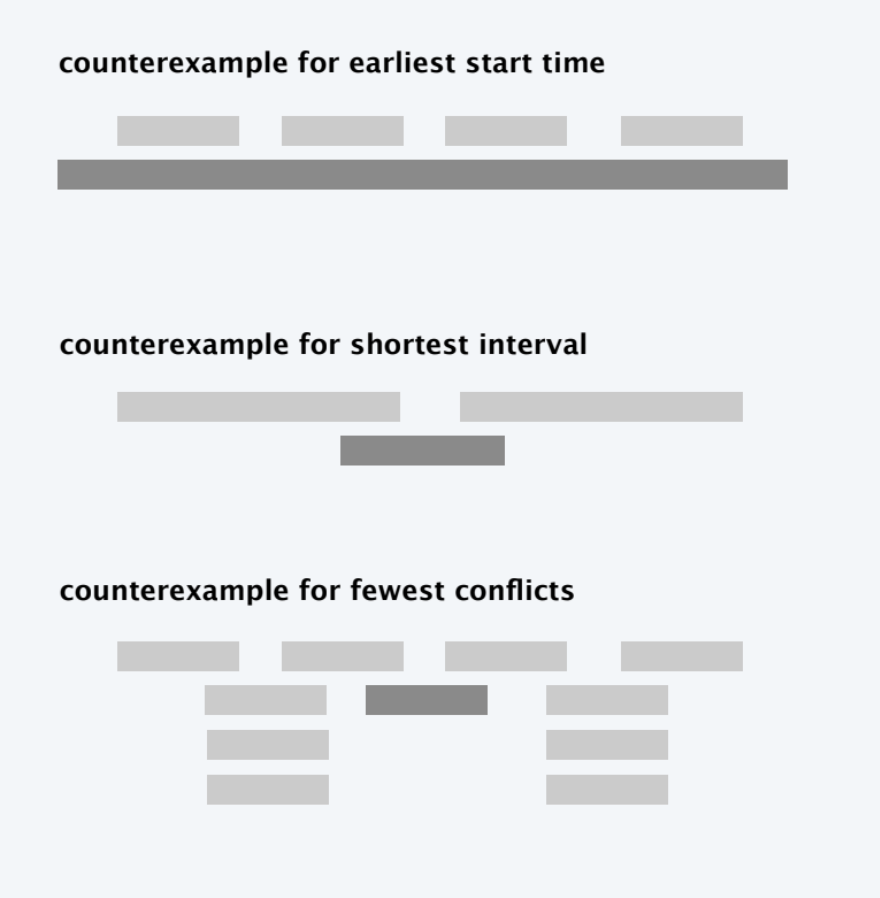
\includegraphics[width=0.4\textwidth]{imm/counterexample.png}
\end{figure}

\subsection{Earliest-Finish-Time-First Algorithm}

\begin{figure}[H]
\centering
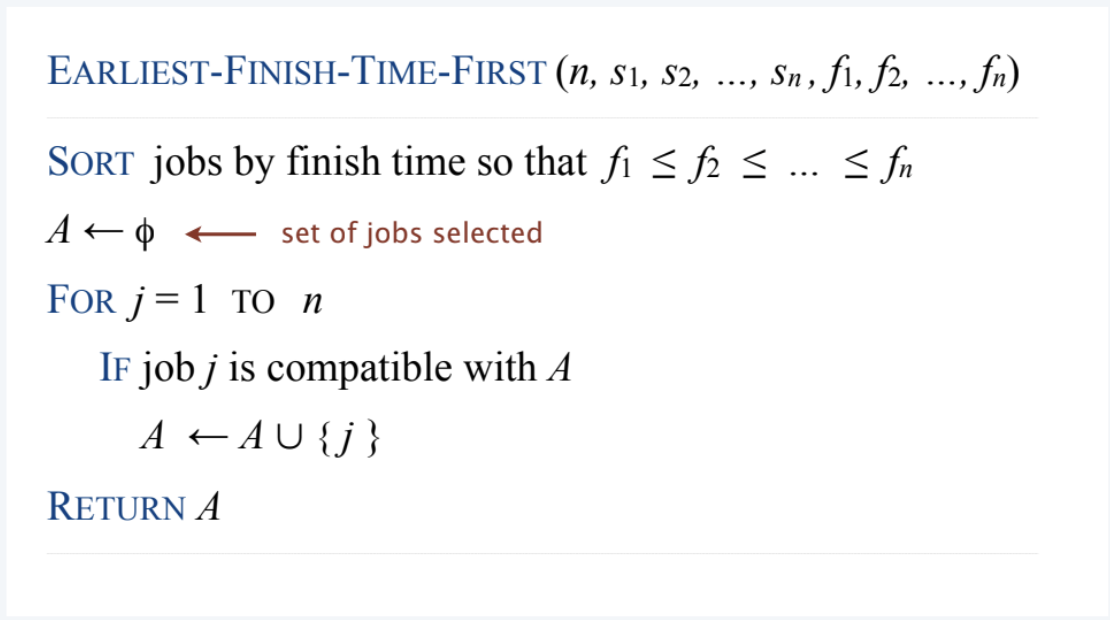
\includegraphics[width=0.9\textwidth]{imm/E_F_T_F.png}
\end{figure}

\noindent
\begin{minipage}[t]{0.3\textwidth}
\vspace{0pt}
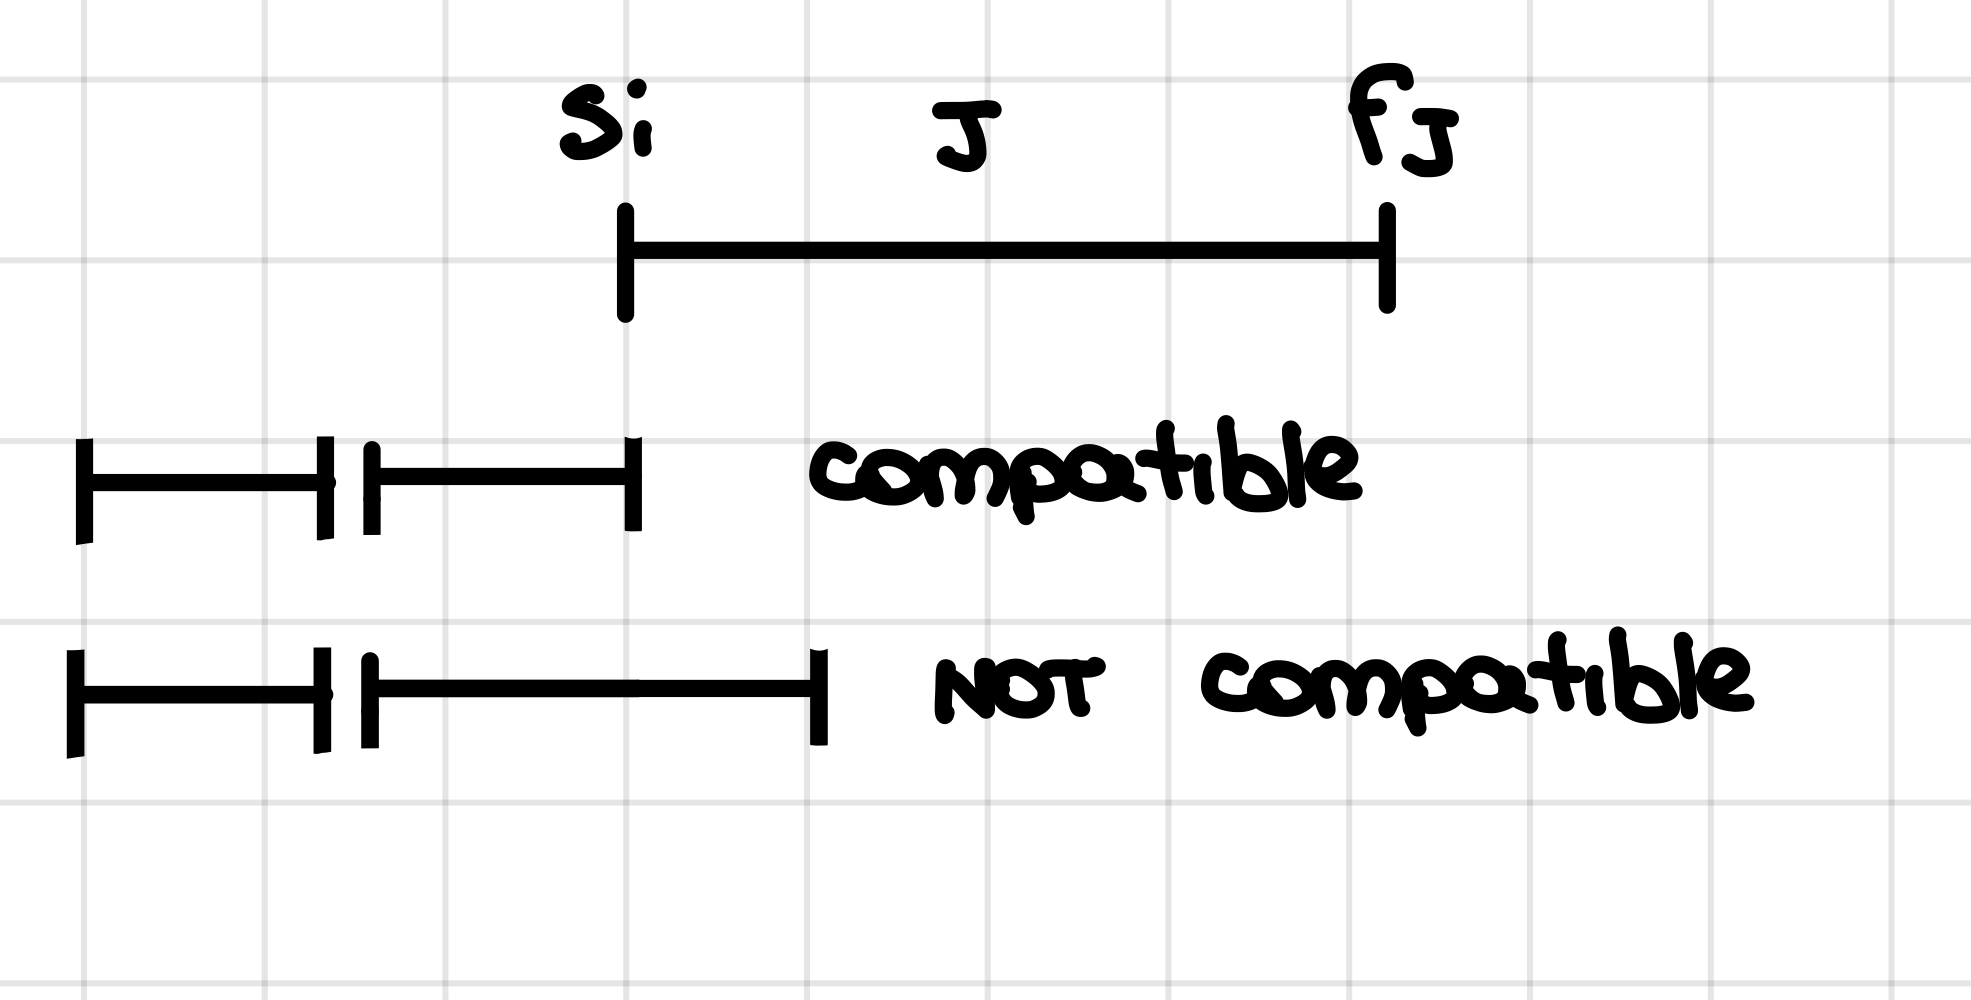
\includegraphics[width=\textwidth]{imm/Immagine JPEG-4835-9E45-EC-0.jpeg}
\end{minipage}%
\hfill
\begin{minipage}[t]{0.65\textwidth}
\vspace{0pt}
\textbf{Implementation note.} Keep track of the last job $j^*$ added to $A$. Job $j$ is compatible
with $A$ if and only if $s_j \geq f_{j^*}$. Sorting takes $O(n \log n)$ time; the loop is $O(n)$.
Total: $O(n \log n)$.
\end{minipage}

\subsection{Proof of Optimality}

\begin{theorem}
The earliest-finish-time-first algorithm is optimal.
\end{theorem}

\begin{proof}[Proof (by contradiction)]
Assume the greedy algorithm is not optimal. Let $i_1, i_2, \ldots, i_k$ be the jobs selected
by the greedy algorithm, and let $j_1, j_2, \ldots, j_m$ be the jobs in an optimal solution with
$i_1 = j_1, i_2 = j_2, \ldots, i_r = j_r$ for the largest possible $r$.
(At $r$, the greedy and optimal solutions first differ.)
If $r = k$, then the greedy solution has $k$ jobs and the optimal has $m \geq k$, so they are
equal (both optimal). Otherwise, job $i_{r+1}$ exists. Since the greedy algorithm picks jobs by
earliest finish time, $f_{i_{r+1}} \leq f_{j_{r+1}}$. We can replace $j_{r+1}$ with $i_{r+1}$
in the optimal solution. This creates a new optimal solution with one more agreement, contradicting
the maximality of $r$.

\begin{figure}[H]
\centering
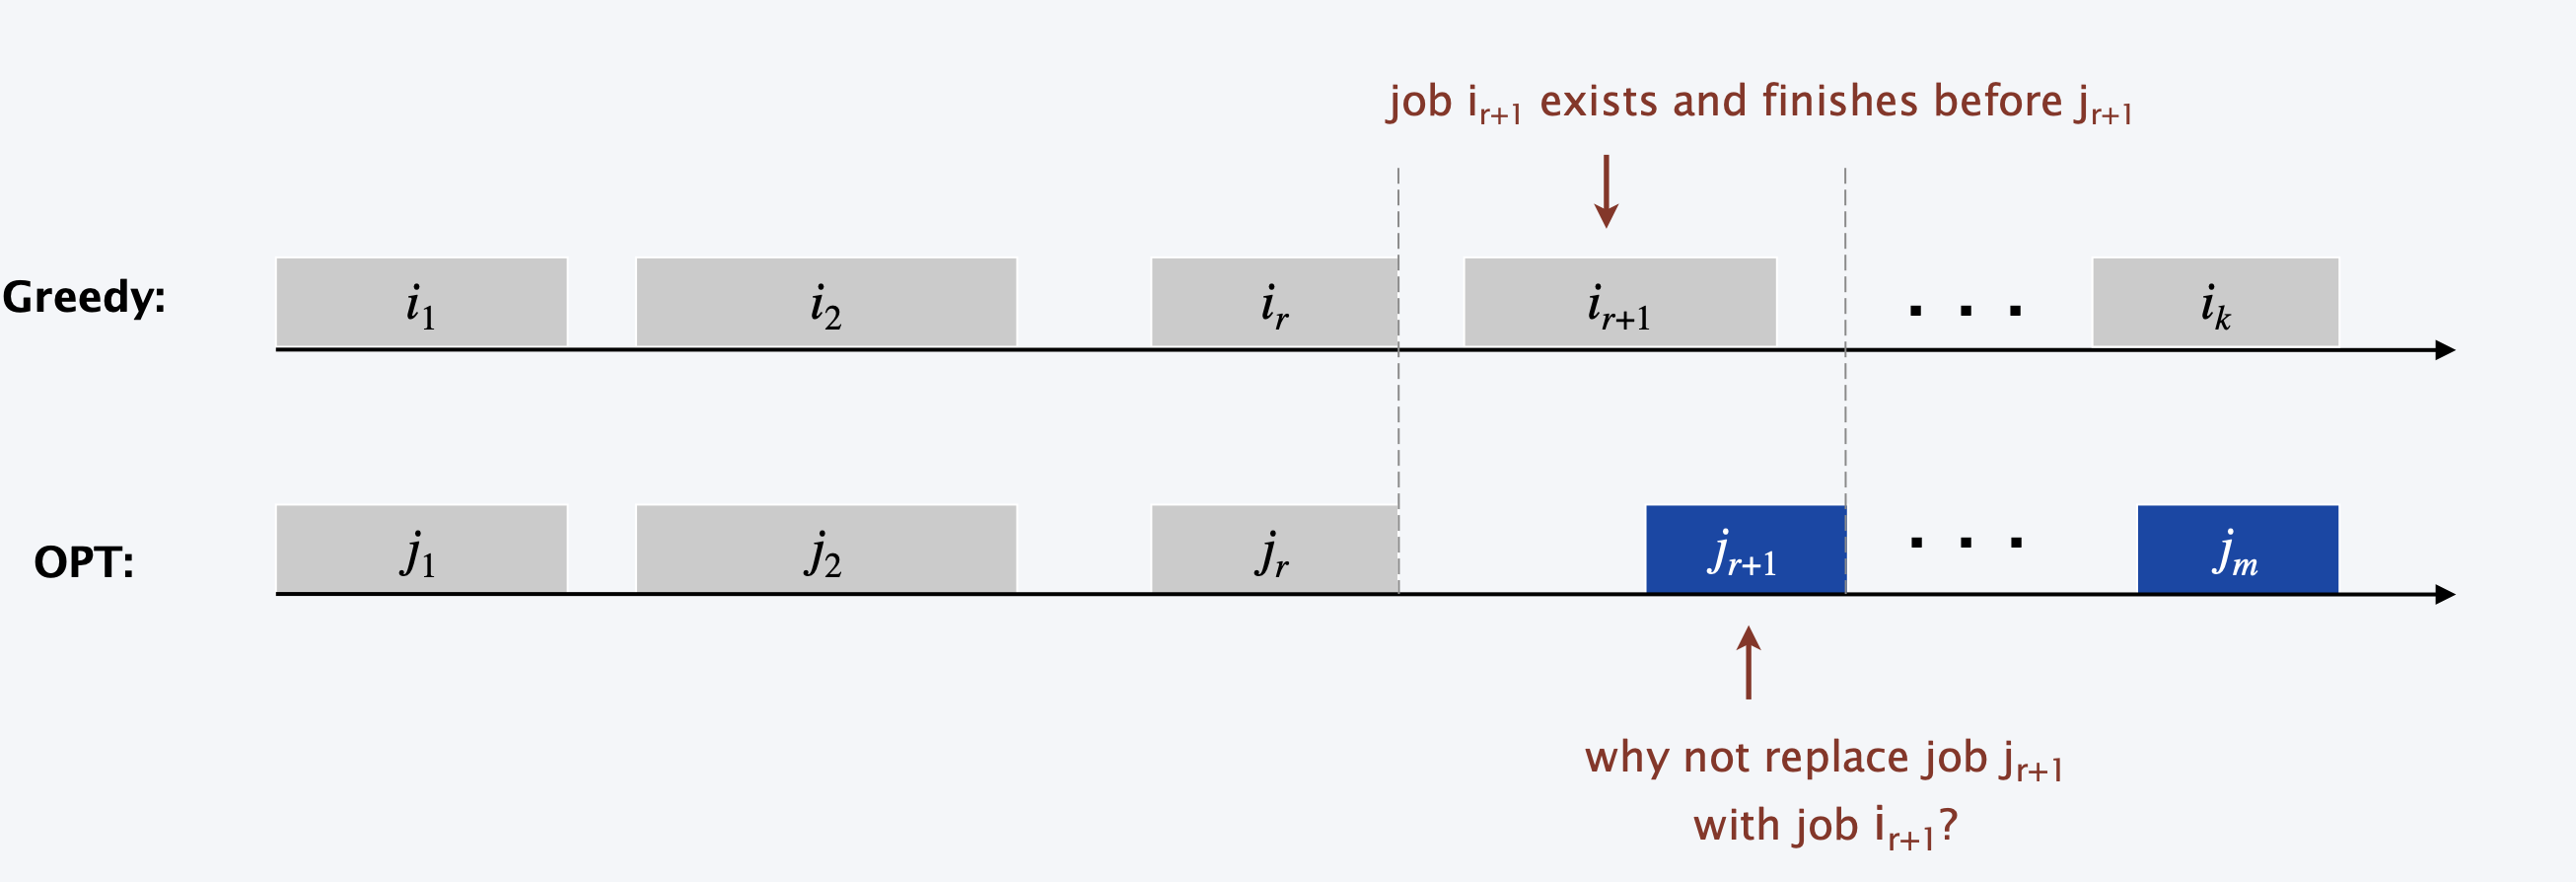
\includegraphics[width=0.7\textwidth]{imm/Screenshot 2026-03-02 alle 19.14.47.png}
\end{figure}
\end{proof}

% ─────────────────────────────────────────────
\section{Interval Partitioning}

\subsection{The Problem}

\textbf{Input.} A set of $n$ lectures. Lecture $j$ starts at $s_j$ and finishes at $f_j$.

\textbf{Goal.} Schedule all lectures using the \emph{minimum number} of classrooms so that no
two lectures overlap in the same classroom.

\begin{figure}[H]
\centering
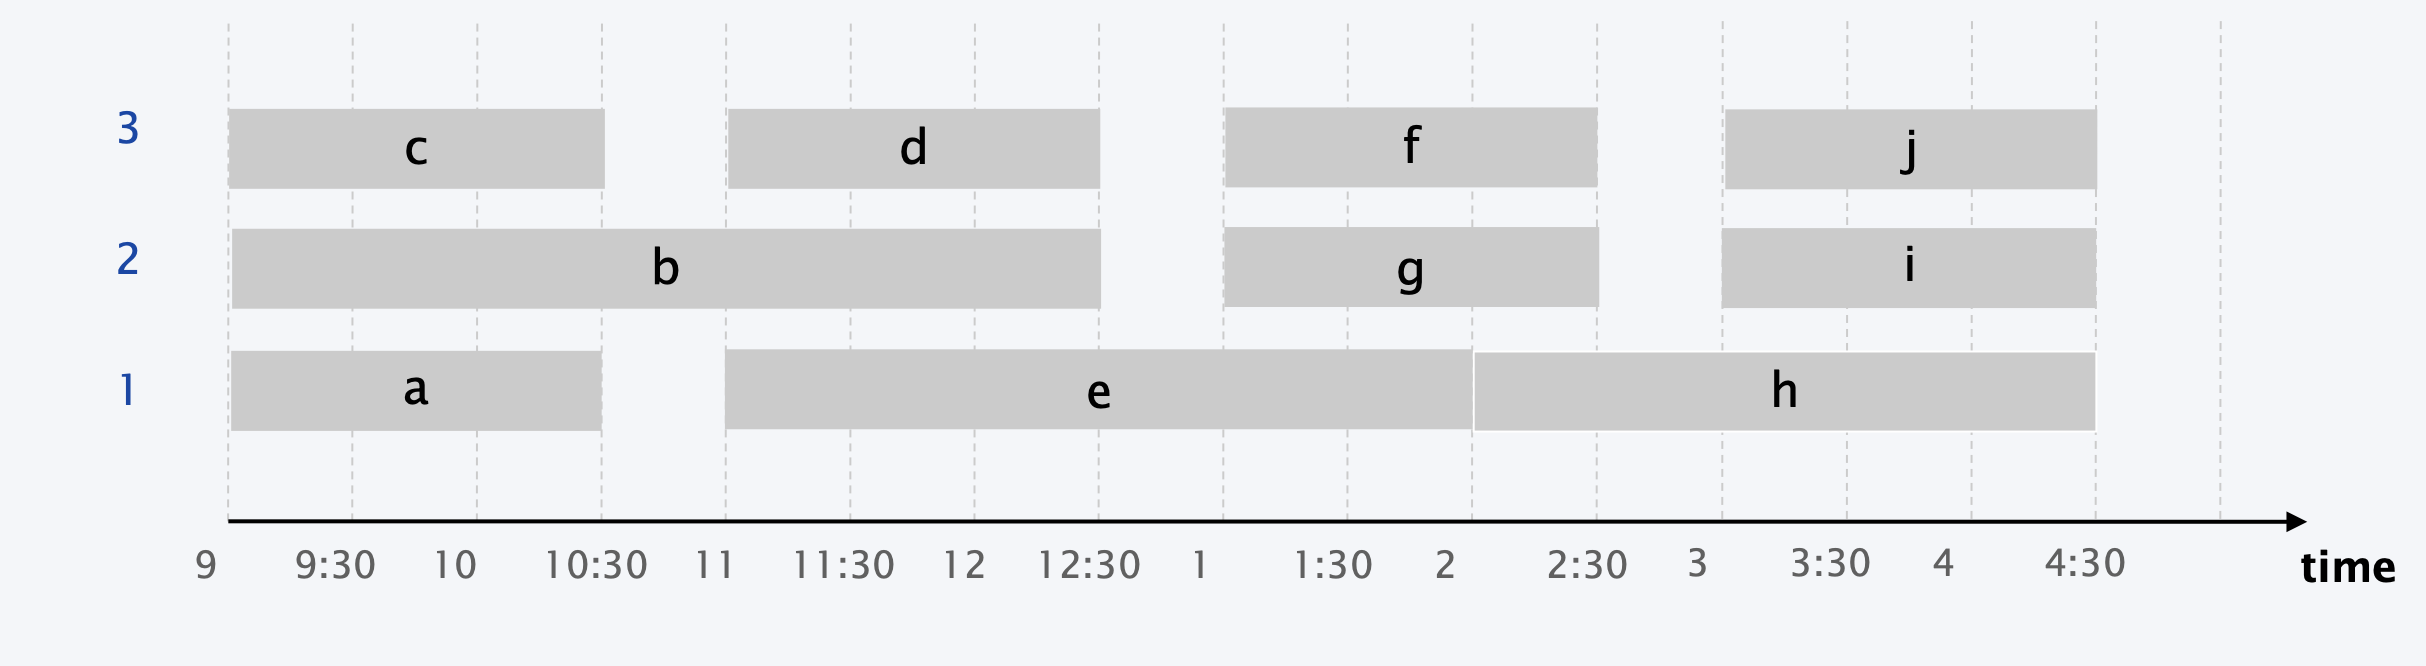
\includegraphics[width=0.7\textwidth]{imm/Screenshot 2026-03-02 alle 19.17.29.png}
\end{figure}

\subsection{Depth and Lower Bound}

\begin{definition}[Depth]
The \emph{depth} of a set of intervals is the maximum number of intervals that contain any given time.
\end{definition}
When we talk about lower bound, we mean a number that is less than or equal to the optimal solution. Since the depth is a lower bound, it means that no schedule can use fewer classrooms than the depth.

\begin{figure}[H]
\centering
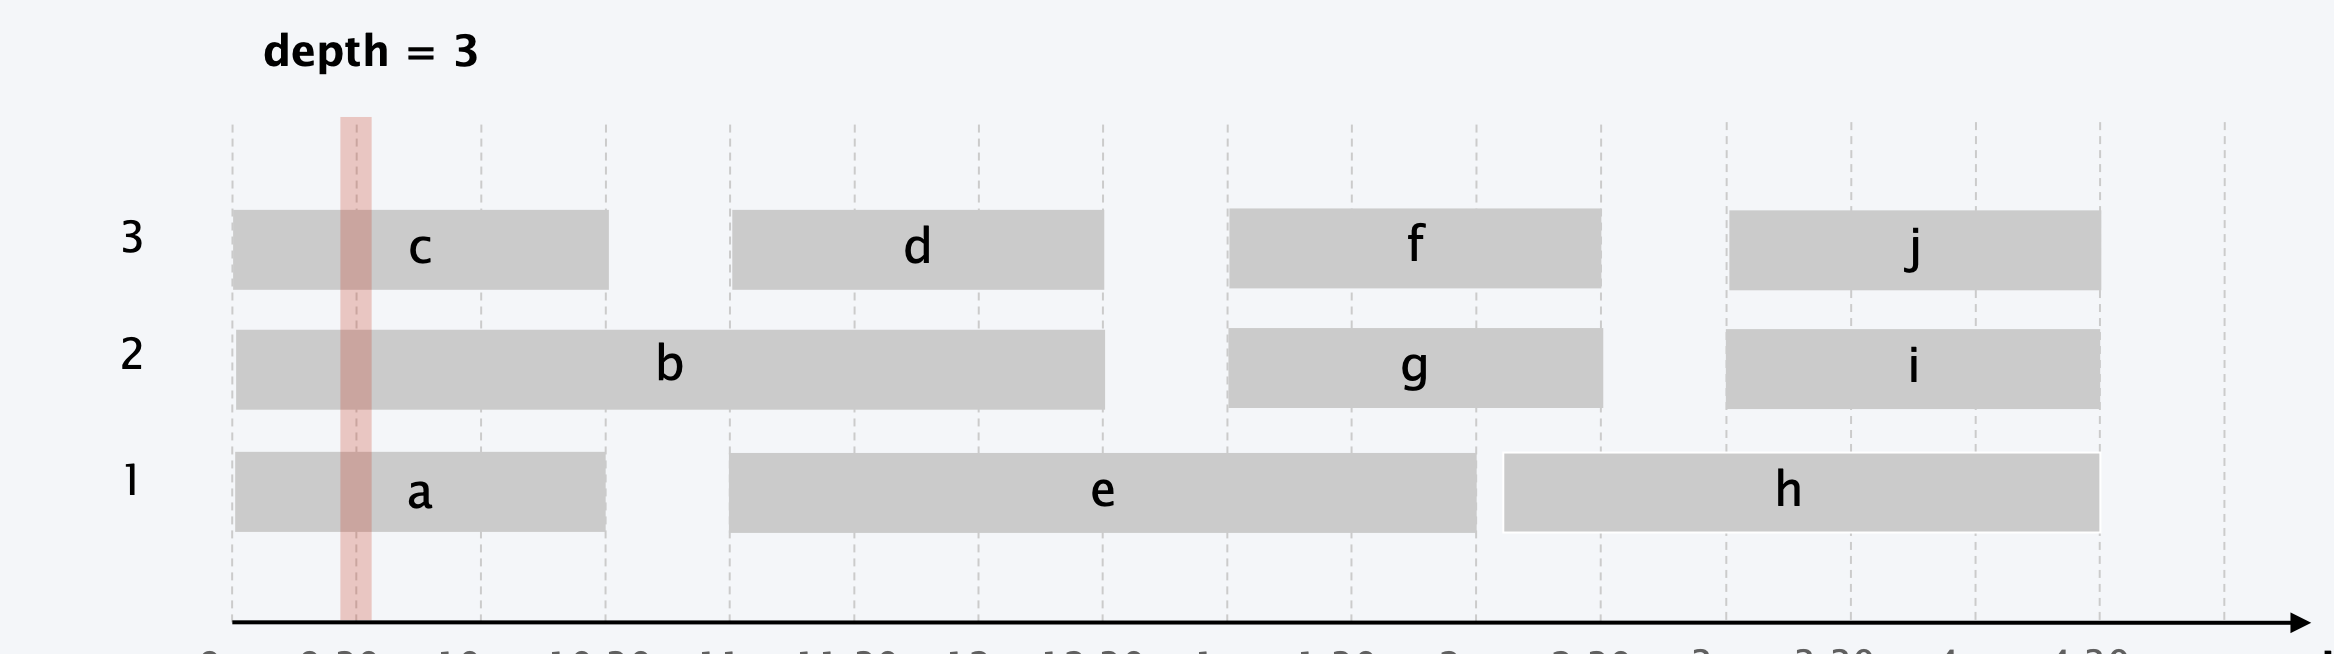
\includegraphics[width=0.7\textwidth]{imm/Screenshot 2026-03-02 alle 19.21.30.png}
\end{figure}

\textbf{Key observation.} The number of classrooms needed is at least the depth.
The optimal number always equal the depth and the earliest-start-time-first algorithm achieves it.

\subsection{Earliest-Start-Time-First Algorithm}

\begin{figure}[H]
\centering
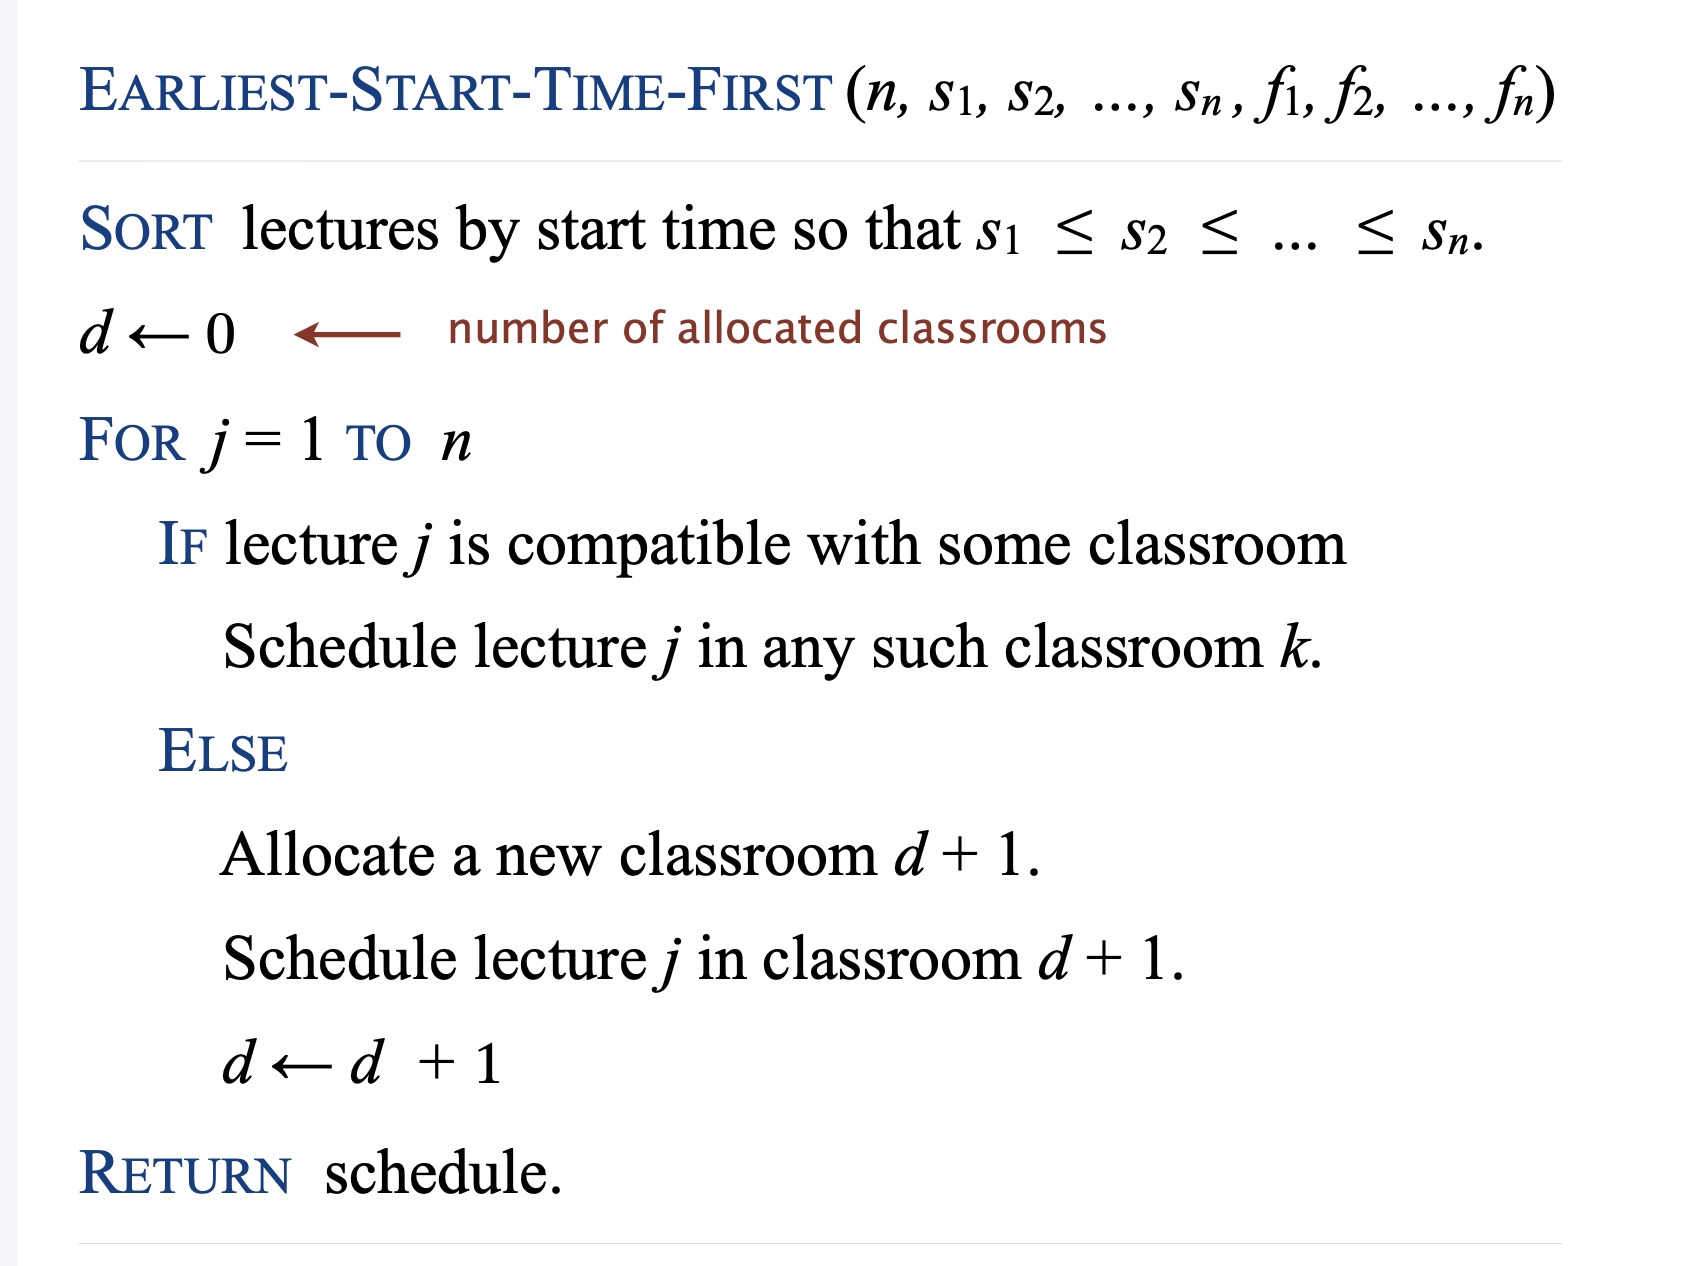
\includegraphics[width=0.9\textwidth]{imm/Screenshot 2026-03-02 alle 19.22.41.png}
\end{figure}

\textbf{Implementation.} Use a priority queue to store classrooms, keyed by the finish time of their
last lecture. To check if lecture $j$ is compatible, compare $s_j$ to the minimum key in the queue.
If compatible, assign $j$ to that classroom and update its key to $f_j$. 
\newline
\textbf{Running time:} Sorting takes $O(n \log n)$. Each of the $n$ lectures is processed once, and each priority queue operation takes $O(\log n)$, so the total is $O(n \log n)$.


\subsection{Proof of Optimality}

\begin{theorem}
The earliest-start-time-first algorithm is optimal.
\end{theorem}

\begin{proof}
Let $d$ be the number of classrooms the algorithm uses. Classroom $d$ was opened because we had
to schedule some lecture $j$ that was incompatible with all $d-1$ existing classrooms. This means
there are $d$ lectures that all overlap at time $s_j + \varepsilon$ (lecture $j$ plus one from
each of the other $d-1$ classrooms). Since these $d$ lectures overlap, any schedule must use at
least $d$ classrooms. The algorithm uses exactly $d$ classrooms, so it is optimal.
\end{proof}

% ─────────────────────────────────────────────
\newpage
\section{Scheduling to Minimize Lateness}

\subsection{The Problem}

\textbf{Input.} A single resource processes one job at a time. Job $j$ requires $t_j$ units of
processing time and has a deadline $d_j$.

\textbf{Definitions.}
\begin{itemize}
    \item If job $j$ starts at time $s_j$, it finishes at time $f_j = s_j + t_j$.
    \item The \emph{lateness} of job $j$ is $\ell_j = \max\{0, f_j - d_j\}$.
\end{itemize}

\textbf{Goal.} Schedule all jobs to minimize the \emph{maximum lateness} $L = \max_j \ell_j$.
\begin{figure}[H]
    \centering
    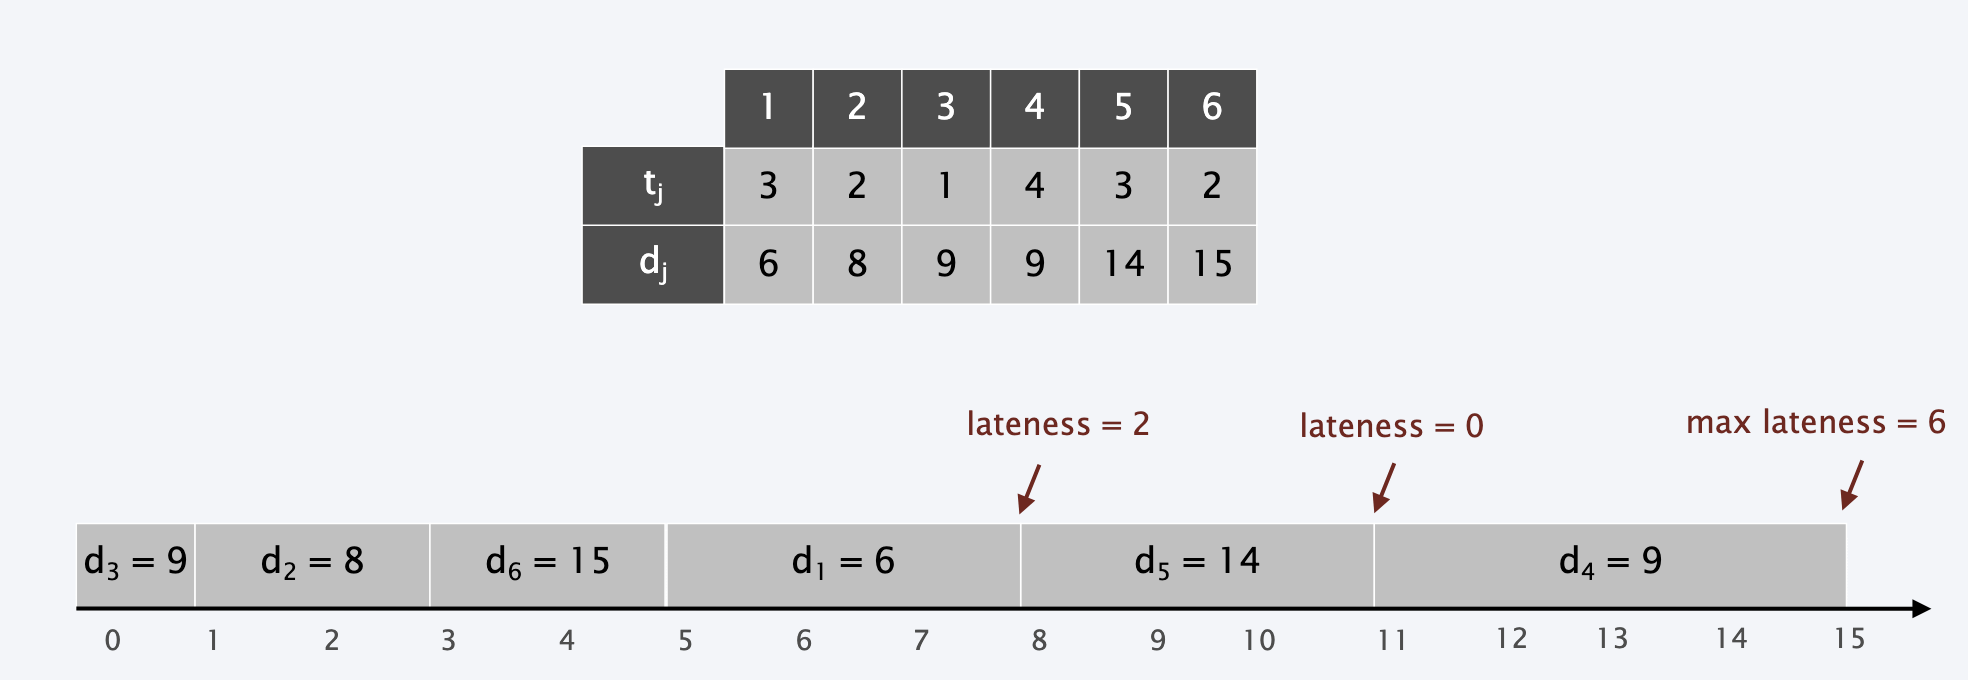
\includegraphics[width=0.9\textwidth]{imm/Screenshot 2026-03-05 alle 13.00.49.png}
\end{figure}
\subsection{Greedy Candidates}

\begin{enumerate}
    \item \textbf{Shortest processing time first:} schedule jobs in ascending order of $t_j$.
    \item \textbf{Earliest deadline first:} schedule jobs in ascending order of $d_j$.
    \item \textbf{Smallest slack:} schedule jobs in ascending order of $d_j - t_j$ (slack = deadline
    minus processing time).
\end{enumerate}

\begin{figure}[H]
\centering
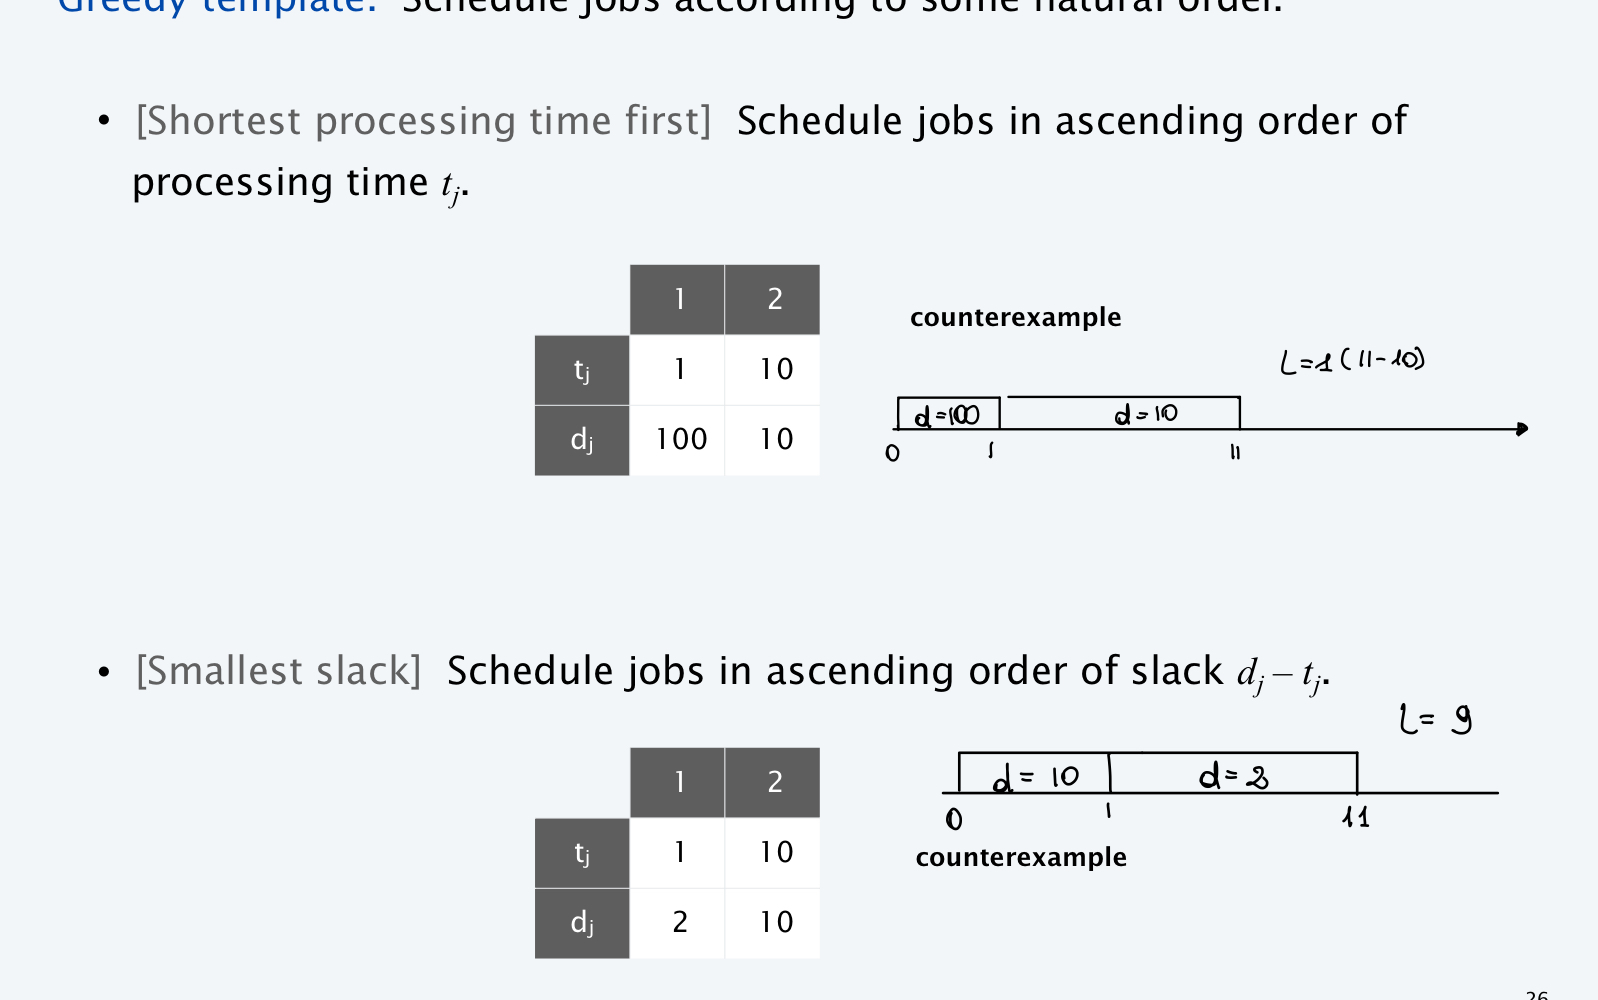
\includegraphics[width=0.5\textwidth]{imm/Immagine JPEG-4277-B732-48-0.jpeg}
\caption{Counterexample showing that only earliest-deadline-first works.}
\end{figure}

\subsection{Earliest-Deadline-First Algorithm}
\begin{figure}[H]

\centering
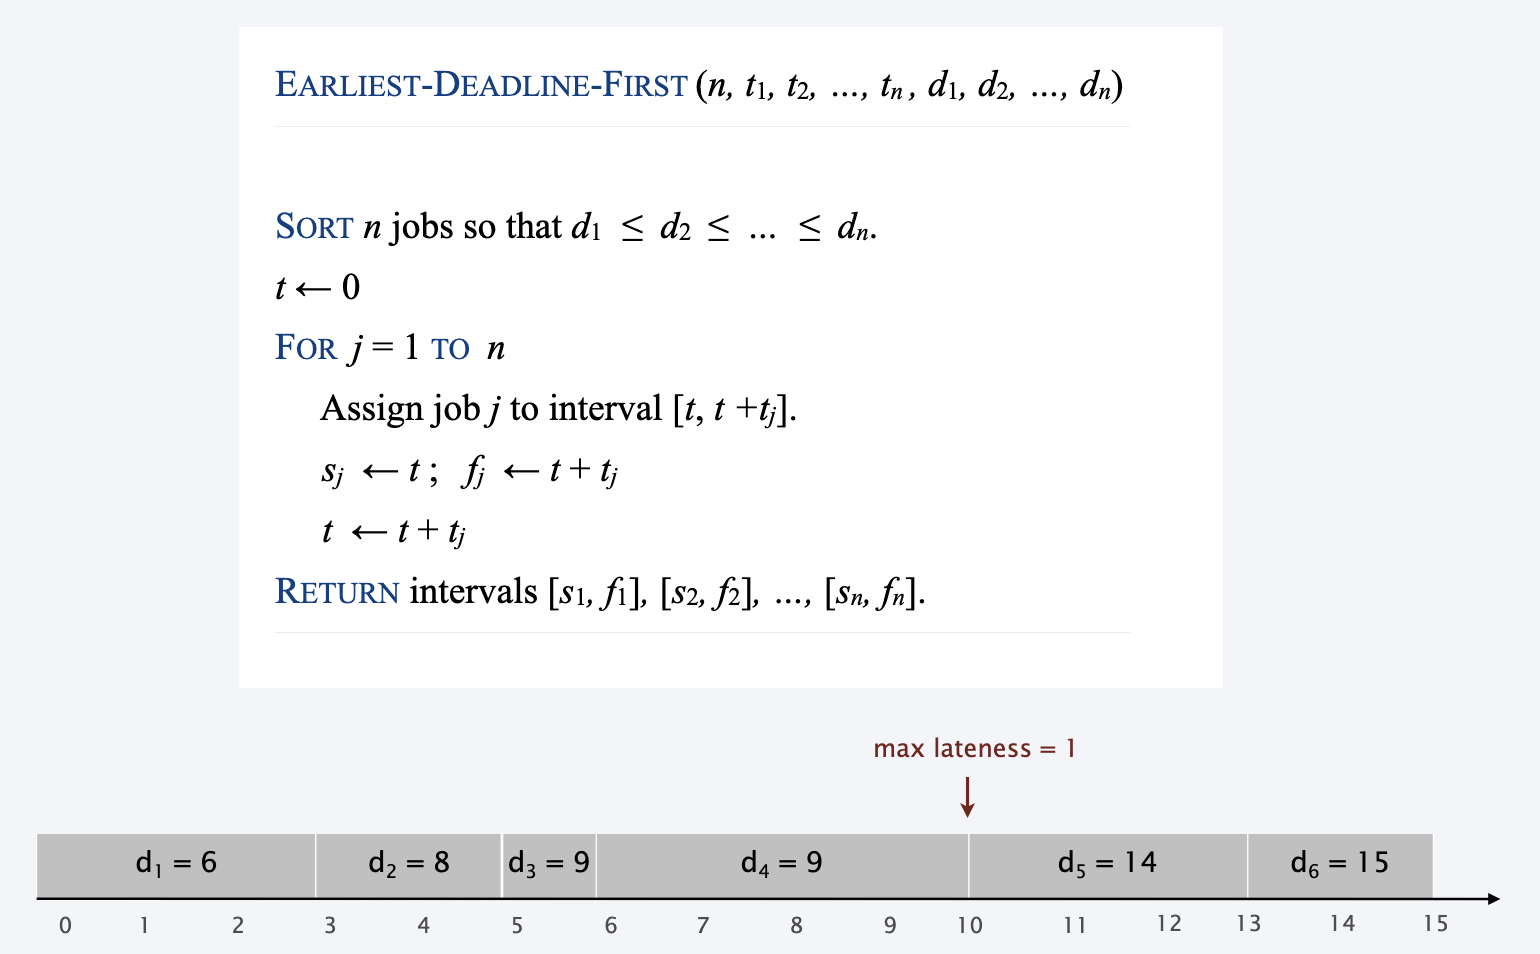
\includegraphics[width=0.8\textwidth]{imm/Screenshot 2026-03-05 alle 13.13.53.png}
\end{figure}

\subsection{Key Observations}

\begin{observation}
There exists an optimal schedule with no idle time.
\begin{figure}[H]
\centering
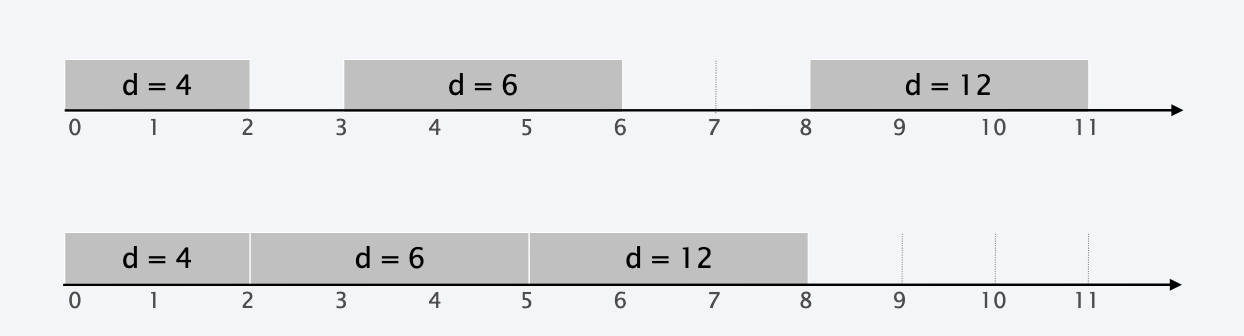
\includegraphics[width=0.5\textwidth]{imm/Screenshot 2026-03-05 alle 13.23.42.png}
\end{figure}
\end{observation}

\begin{observation}
The earliest-deadline-first schedule has no idle time.
\end{observation}

\begin{definition}[Inversion]
Given a schedule $S$ (with jobs numbered so that $d_1 \leq d_2 \leq \cdots \leq d_n$), an
\emph{inversion} is a pair of jobs $i$ and $j$ such that $i < j$ but $j$ is scheduled before $i$.
\end{definition}

\begin{observation}
The earliest-deadline-first schedule has no inversions.
\end{observation}

\begin{observation}
If a schedule (with no idle time) has an inversion, it has one with a pair of inverted jobs
scheduled consecutively.
\end{observation}

\subsection{Exchange Argument}

\begin{claim}
Swapping two adjacent, \textbf{inverted} jobs reduces the number of inversions by one and does not increase
the maximum lateness.
\end{claim}

\begin{proof}
Let $\ell$ be the lateness before the swap, and $\ell'$ after.
\newline
Let $i < j$ be the inverted pair
(so $d_i \leq d_j$). For all $k \neq i, j$, we have $\ell'_k = \ell_k$. Job $i$ now finishes
earlier, so $\ell'_i \leq \ell_i$. For job $j$, if it is late:
\[
    \ell'_j = f'_j - d_j = f_i - d_j \leq f_i - d_i \leq \ell_i,
\]
where the first inequality uses $d_i \leq d_j$ (since $i < j$). So the maximum lateness does
not increase.
\end{proof}

\subsection{Proof of Optimality}

\begin{theorem}
The earliest-deadline-first schedule is optimal.
\end{theorem}

\begin{proof}[Proof (by contradiction)]
Let $S^*$ be an optimal schedule with the fewest number of inversions. We can assume $S^*$ has no
idle time. If $S^*$ has no inversions, then $S^* = S_{\text{EDF}}$ and we are done. Otherwise,
let $i$--$j$ be an adjacent inversion in $S^*$. Swapping $i$ and $j$ does not increase the maximum
lateness and strictly decreases the number of inversions. This contradicts the assumption that
$S^*$ has the fewest inversions among optimal schedules.
\end{proof}


% ─────────────────────────────────────────────
\section{Greedy Analysis Strategies}

We have seen three main techniques for proving that a greedy algorithm is optimal:

\begin{enumerate}
    \item \textbf{Greedy stays ahead.} Show that after each step, the greedy solution is at least
    as good as any other solution.

    \emph{Example:} Interval scheduling (earliest-finish-time-first).

    \item \textbf{Structural bound.} Identify a simple lower bound that every solution must satisfy,
    then show that the greedy algorithm achieves this bound.

    \emph{Example:} Interval partitioning (depth = lower bound on number of classrooms).

    \item \textbf{Exchange argument.} Gradually transform any optimal solution into the greedy
    solution by making small changes (``exchanges'') that do not worsen the objective.

    \emph{Examples:} Minimizing lateness (swapping inversions), Optimal caching (changing eviction
    decisions).
\end{enumerate}

\textbf{Other famous greedy algorithms:} Gale--Shapley (stable matching), Kruskal and Prim (minimum
spanning tree), Dijkstra (shortest paths), Huffman (data compression), and many more.

\chapter{ Dynamic Programming}

\section{Algorithmic Paradigms}

There are three main design strategies for algorithms:

\begin{enumerate}
    \item \textbf{Greedy.} Build a solution step by step, always making the locally best
    choice at each step.
    \item \textbf{Divide-and-conquer.} Split the problem into \emph{independent}
    subproblems, solve each one, and combine the results.
    \item \textbf{Dynamic programming.} Split the problem into \emph{overlapping}
    subproblems, solve each one once, and store the result for later reuse.
\end{enumerate}

Dynamic programming is essentially a fancy name for \emph{caching intermediate results in
a table} so they do not have to be recomputed. The key difference from divide-and-conquer
is that subproblems overlap: the same subproblem appears in many branches of the recursion.


%────────────────────────────────────────────────────────────
\section{Weighted Interval Scheduling}

\subsection{Problem Definition}

\textbf{Input.} A set of $n$ jobs. Job $j$ starts at time $s_j$, finishes at $f_j$, and
has value (weight) $v_j > 0$. Two jobs are \emph{compatible} if they do not overlap.

\textbf{Goal.} Find a maximum-weight subset of mutually compatible jobs.

\begin{figure}[H]
\centering
\begin{minipage}{0.45\textwidth}
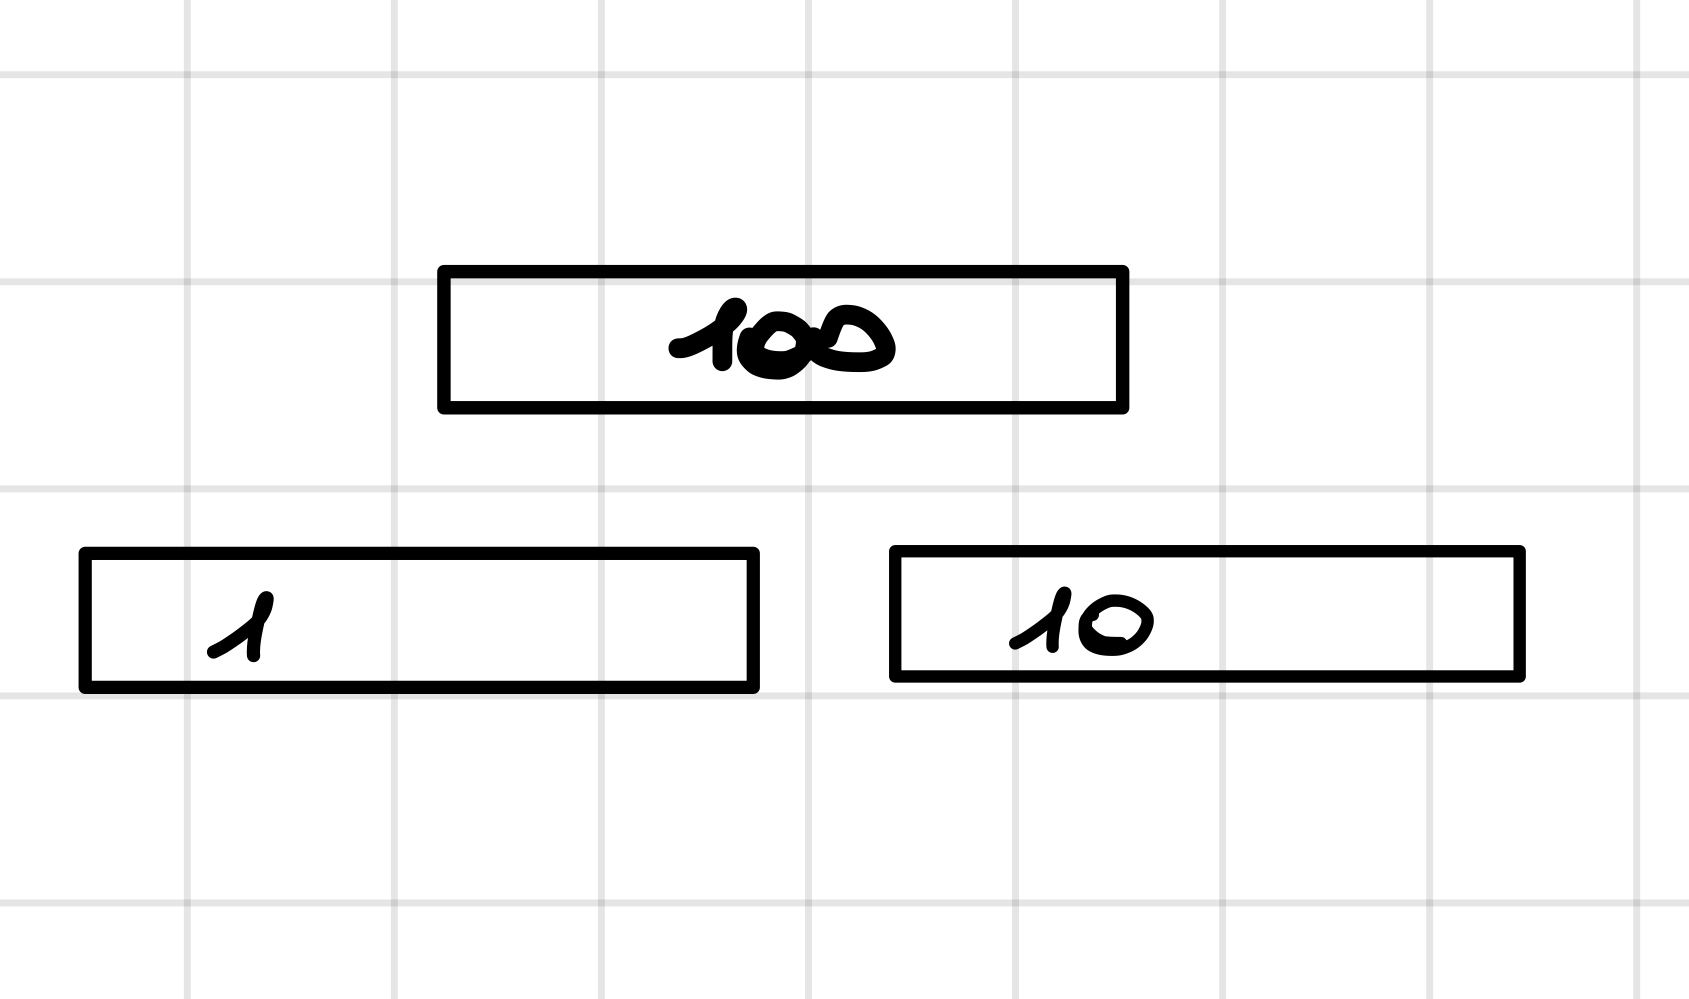
\includegraphics[width=\textwidth]{imm/Immagine JPEG-40DA-B0D9-F4-0.jpeg}
\end{minipage}%
\hfill
\begin{minipage}{0.5\textwidth}
\textbf{Why greedy fails.}\
Counterexample showing that earliest-finish-time-first fails when jobs have weights because a single high-weight job (e.g.
v=100) that overlaps with many low-weight jobs will be ignored by greedy, even though it is clearly the best choice.
\end{minipage}
\end{figure}

\subsection{Key Definitions}

Label jobs by finishing time: $f_1 \leq f_2 \leq \cdots \leq f_n$.

\begin{definition}[Compatible predecessor $p(j)$]
\vspace{0.7em}
$p(j)$ is the largest index $i < j$ such that job $i$ is compatible with job $j$
(i.e., $f_i \leq s_j$). If no such job exists, $p(j) = 0$.
\end{definition}

\textbf{Example.} For a set of 8 jobs: $p(8) = 5$, $p(7) = 3$, $p(2) = 0$.
\begin{figure}[H]
\centering
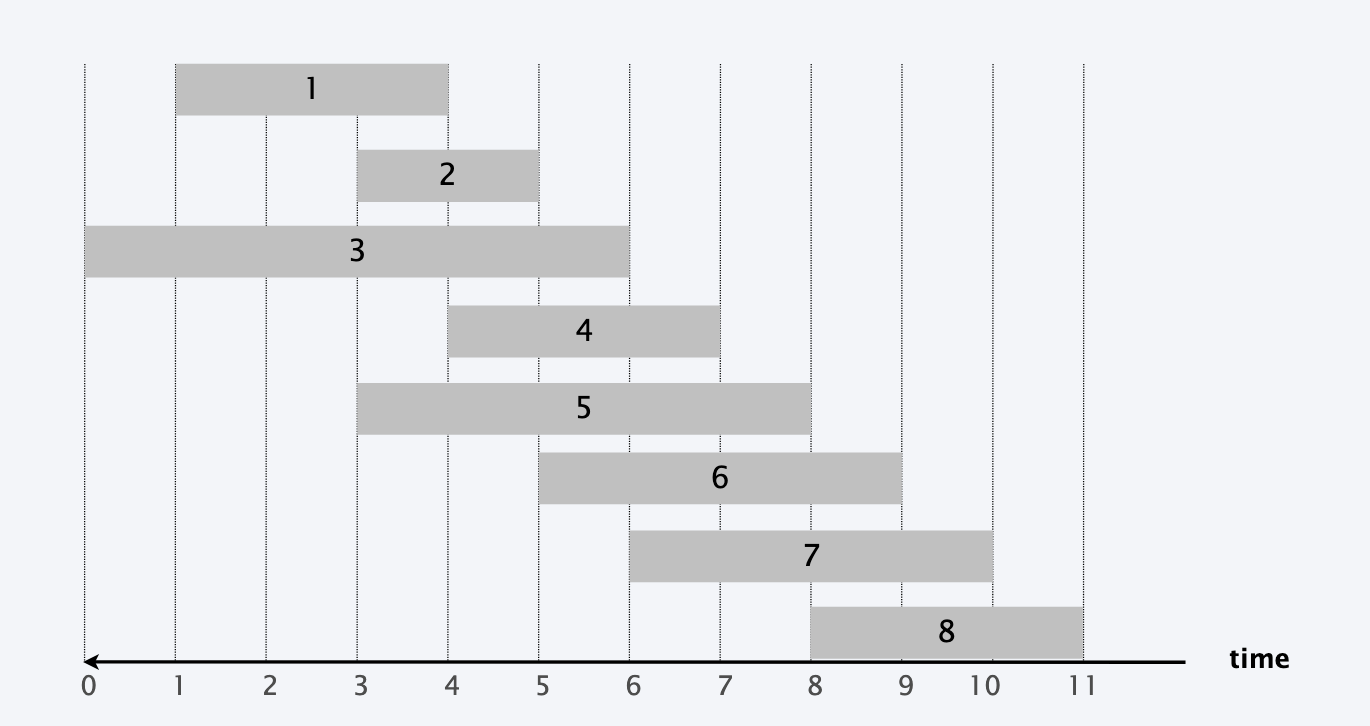
\includegraphics[width=0.7\textwidth]{imm/Screenshot 2026-03-12 alle 12.22.06.png}
\end{figure}
\subsection{Optimal Substructure (Binary Choice)}

\begin{definition}
$\text{OPT}(j)$ = value of the optimal solution using only jobs $1, 2, \ldots, j$.
\end{definition}

For the last job $j$, there are exactly two cases:
\begin{enumerate}
    \item \textbf{OPT does not select job $j$.} Then $\text{OPT}(j) = \text{OPT}(j-1)$.
    \item \textbf{OPT selects job $j$.} Then we collect profit $v_j$ and can no longer
    use jobs $\{p(j)+1, \ldots, j-1\}$. We must solve optimally for jobs $1, \ldots, p(j)$.
    So $\text{OPT}(j) = v_j + \text{OPT}(p(j))$.
\end{enumerate}

\[
    \text{OPT}(j) =
    \begin{cases}
        0 & \text{if } j = 0 \\
        \max\bigl\{v_j + \text{OPT}(p(j)),\; \text{OPT}(j-1)\bigr\} & \text{otherwise}
    \end{cases}
\]

This recurrence has the \emph{optimal substructure property} (proved via exchange argument).
This is a \textbf{binary choice}: either take job $j$ or leave it.

\subsection{Brute Force}
\begin{figure}[H]
\centering
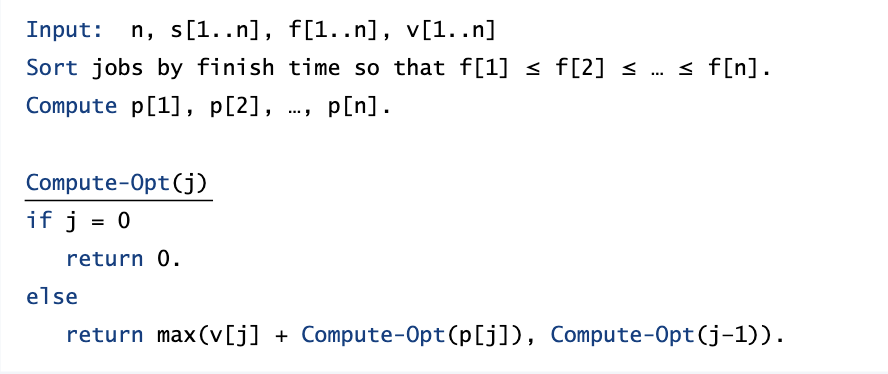
\includegraphics[width=0.9\textwidth]{imm/Screenshot 2026-03-12 alle 12.29.45.png}
\end{figure}

A naive recursive implementation recomputes the same subproblems many times. For a

In pratica, $p(j) = j-2$ significa che il lavoro $j$ è compatibile solo con il lavoro $j-2$ (mentre $j-1$ si sovrappone a $j$ e non può essere scelto insieme a $j$).Questo rende la ricorsione simile a quella dei numeri di Fibonacci, perché ogni soluzione dipende da due sottoproblemi distinti.
n = 5, $p(5) = 3$ significa che il lavoro 5 è compatibile solo con il lavoro 3 (e non con il lavoro 4). Quindi, quando consideriamo se includere il lavoro 5, dobbiamo guardare alla soluzione ottimale per i primi 3 lavori (OPT(3)) invece che per i primi 4 lavori (OPT(4)). In questo caso, OPT(5) dipende da OPT(3) e OPT(4), e OPT(4) dipende da OPT(2) e OPT(3), e così via, creando una struttura ricorsiva che porta a molte chiamate ripetute degli stessi sottoproblemi.

\begin{figure}[H]
\centering
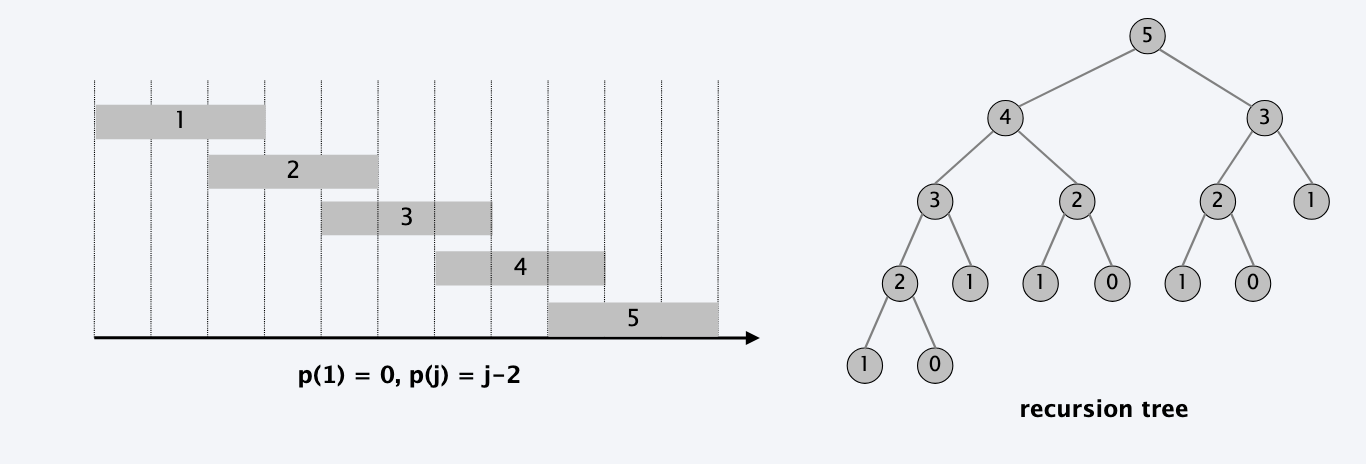
\includegraphics[width=0.9\textwidth]{imm/Screenshot 2026-03-12 alle 12.35.59.png}
\end{figure}

\subsection{Memoization: Top-Down DP}

\textbf{Key idea.} Cache the result of each subproblem the first time it is computed, and
look it up directly on future calls.
\begin{figure}[H]
\centering
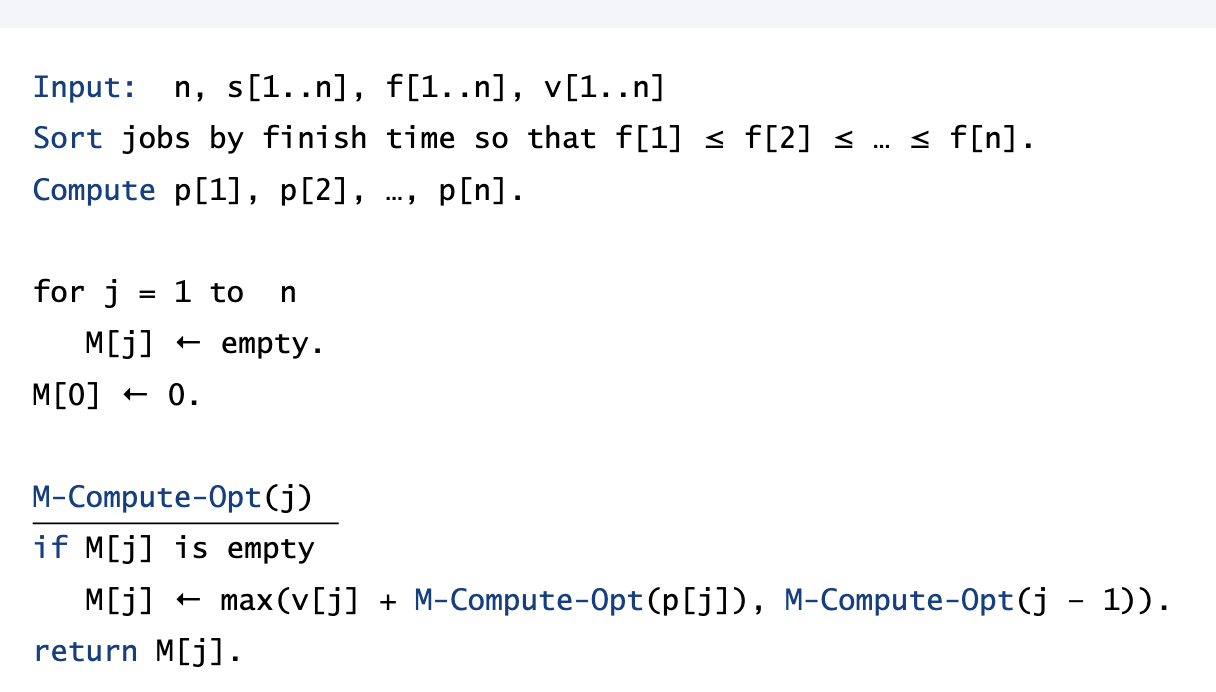
\includegraphics[width=0.9\textwidth]{imm/Screenshot 2026-03-12 alle 12.36.37.png}
\end{figure}

\begin{claim}
The memoized algorithm runs in $O(n \log n)$ time.
\end{claim}

\begin{proof}
Sorting by finish time: $O(n \log n)$. Computing $p(\cdot)$: $O(n \log n)$ via binary
search after sorting by start time. Each call to \textsc{M-Compute-Opt}$(j)$ either
(i) returns an existing value in $O(1)$, or (ii) fills in a new entry and makes two
recursive calls. Let $\Phi$ = number of non-empty entries in $M$: initially $\Phi = 0$,
and case (ii) increases $\Phi$ by 1. Since $\Phi \leq n$ throughout, there are at most
$2n$ recursive calls of type (ii), so \textsc{M-Compute-Opt}$(n)$ uses $O(n)$ time after
preprocessing.
\end{proof}

\subsection{Finding the Actual Solution}

The DP computes the optimal \emph{value}. To recover the actual \emph{set of jobs}, do a
second pass:

\begin{figure}[H]
\centering
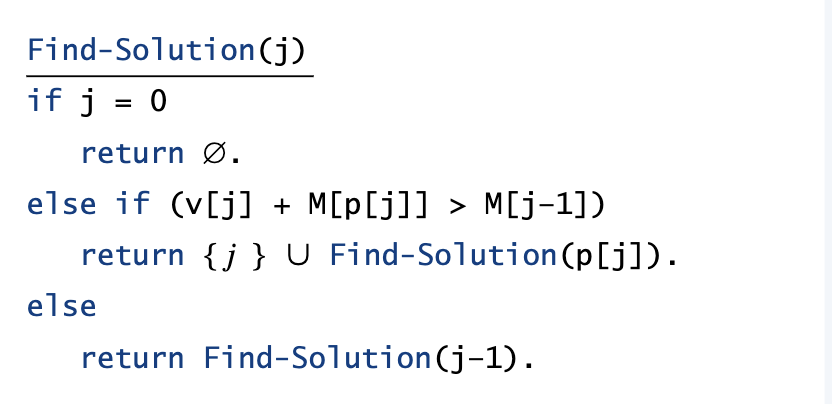
\includegraphics[width=0.9\textwidth]{imm/Screenshot 2026-03-17 alle 17.51.54.png}
\end{figure}

At most $n$ recursive calls, so $O(n)$ time.

\subsection{Bottom-Up DP}

Instead of recursion with memoization (top-down), we can fill the table iteratively
from small to large (bottom-up):

\begin{figure}[H]
\centering
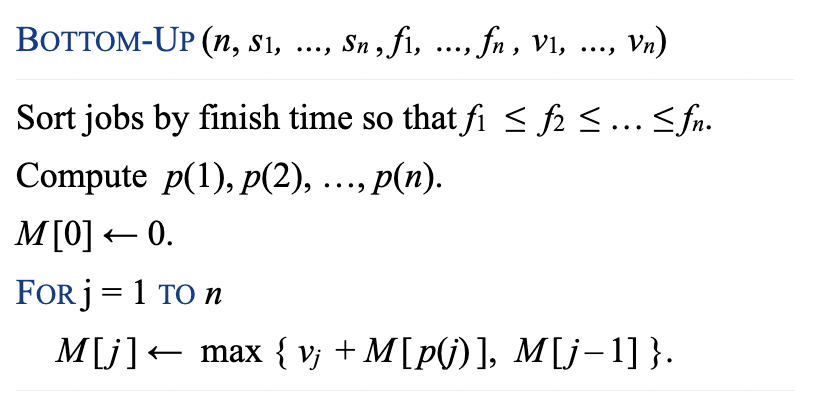
\includegraphics[width=0.9\textwidth]{imm/Screenshot 2026-03-17 alle 18.04.43.png}
\end{figure}


Bottom-up and top-down (with memoization) produce the same table. The choice between them
is largely a matter of personal style and the specific problem.

%────────────────────────────────────────────────────────────
\section{Segmented Least Squares}

\subsection{Background: Least Squares}

Given $n$ points $(x_1, y_1), \ldots, (x_n, y_n)$ in the plane, the \textbf{least squares}
line $y = ax + b$ minimises the sum of squared errors:
\[
    \text{SSE} = \sum_{i=1}^{n} (y_i - ax_i - b)^2.
\]
Calculus gives the closed-form solution:
\[
    a = \frac{n \sum_i x_i y_i - (\sum_i x_i)(\sum_i y_i)}
            {n \sum_i x_i^2 - (\sum_i x_i)^2},
    \qquad
    b = \frac{\sum_i y_i - a \sum_i x_i}{n}.
\]

\subsection{Problem Definition}

In practice, data often follows \emph{several} line segments, not a single line.

\textbf{Input.} $n$ points $(x_1, y_1), \ldots, (x_n, y_n)$ with $x_1 < x_2 < \cdots < x_n$,
and a penalty constant $c > 0$.

\textbf{Goal.} Find a sequence of line segments that minimises:
\[
    f = E + cL,
\]
where $E$ is the total sum of squared errors across all segments, and $L$ is the number of
segments. The constant $c$ controls the trade-off between \emph{accuracy} (small $E$) and
\emph{parsimony} (small $L$).

\subsection{Optimal Substructure (Multiway Choice)}

\begin{definition}
\begin{itemize}
   
    \item $e(i, j)$ = minimum sum of squared errors for points $p_i, p_{i+1}, \ldots, p_j$
    (the cost of fitting a single line to this segment).
     \item $\text{OPT}(j)$ = minimum cost for points $p_1, p_2, \ldots, p_j$.
\end{itemize}
\end{definition}


The last segment must end at $p_j$ and start at some $p_i$. For each choice of $i$:
\[
    \text{cost} = e(i, j) + c + \text{OPT}(i - 1).
\]

This gives the recurrence:
\[
    \text{OPT}(j) =
    \begin{cases}
        0 & \text{if } j = 0 \\
        \displaystyle\min_{1 \leq i \leq j} \bigl\{ e(i, j) + c + \text{OPT}(i-1) \bigr\}
        & \text{otherwise}
    \end{cases}
\]

This is a \textbf{multiway choice}: we choose \emph{which point} to start the last segment
from, not just a binary yes/no.

\subsubsection*{Example}

Consider four points sorted by their $x$-coordinates:
\[
p_1=(1,1), \quad p_2=(2,2), \quad p_3=(3,2), \quad p_4=(4,4).
\]
Let the penalty for each segment be $c=1$.

Assume the following precomputed least-squares errors:
\[
e_{1,1}=0,\ e_{1,2}=0.5,\ e_{1,3}=1.2,\ e_{1,4}=3.0,
\]
\[
e_{2,2}=0,\ e_{2,3}=0.2,\ e_{2,4}=1.5,
\]
\[
e_{3,3}=0,\ e_{3,4}=0.4,\qquad e_{4,4}=0.
\]

We define $OPT(j)$ as the minimum cost of approximating the first $j$ points. The dynamic programming recurrence is
\[
OPT(j)=\min_{1\le i\le j}\bigl(e_{i,j}+c+OPT(i-1)\bigr),
\qquad OPT(0)=0.
\]

Now compute the values:
\[
OPT(1)=e_{1,1}+c+OPT(0)=0+1+0=1,
\]
\[
OPT(2)=\min\{e_{1,2}+1+OPT(0),\ e_{2,2}+1+OPT(1)\}
       =\min\{1.5,\ 2\}=1.5,
\]
\[
OPT(3)=\min\{e_{1,3}+1+OPT(0),\ e_{2,3}+1+OPT(1),\ e_{3,3}+1+OPT(2)\}
       =\min\{2.2,\ 2.2,\ 2.5\}=2.2,
\]
\[
OPT(4)=\min\{e_{1,4}+1+OPT(0),\ e_{2,4}+1+OPT(1),\ e_{3,4}+1+OPT(2),\ e_{4,4}+1+OPT(3)\}
\]
\[
       =\min\{4.0,\ 3.5,\ 3.9,\ 3.2\}=3.2.
\]

Therefore, the optimal cost for all four points is $OPT(4)=3.2$.
\subsection{Algorithm}

\begin{figure}[H]
\centering
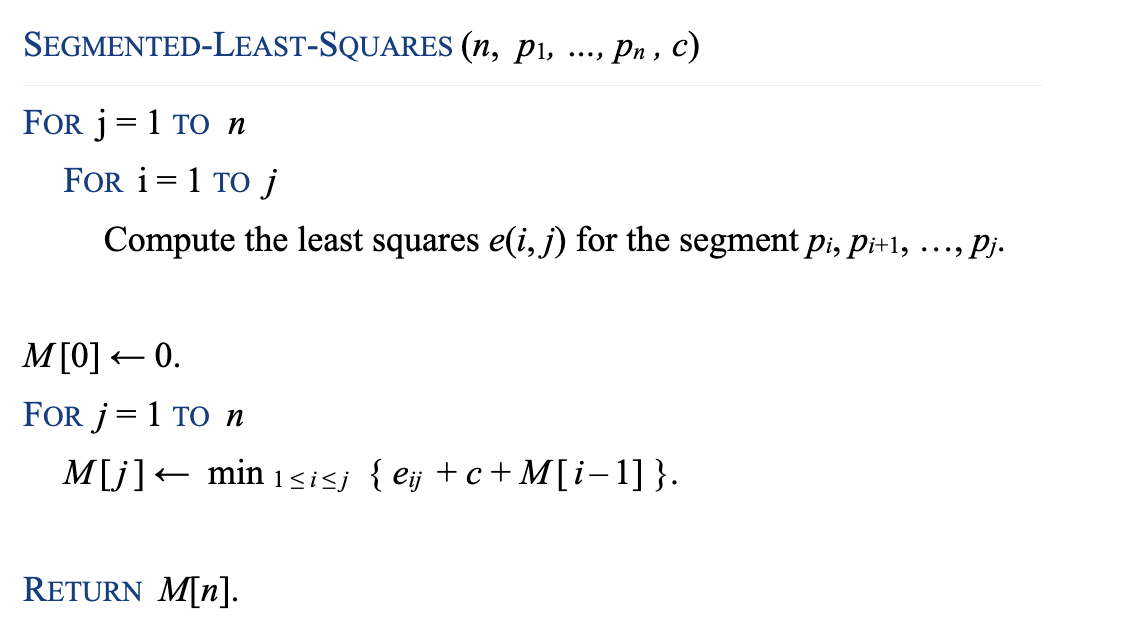
\includegraphics[width=0.9\textwidth]{imm/Screenshot 2026-03-17 alle 18.06.31.png}
\end{figure}

\begin{theorem}[Bellman 1961]
The DP algorithm solves the segmented least squares problem in $O(n^3)$ time and $O(n^2)$ space.
\end{theorem}

\begin{proof}
There are $O(n^2)$ pairs $(i, j)$. Computing $e(i, j)$ for each pair takes $O(n)$ time using
the closed-form formula. The bottleneck is therefore $O(n^2) \times O(n) = O(n^3)$.
\end{proof}


By precomputing prefix sums $\sum x_i$, $\sum y_i$, $\sum x_i y_i$, $\sum x_i^2$, each
$e(i, j)$ can be computed in $O(1)$, reducing the total to $O(n^2)$ time and $O(n)$ space.

%────────────────────────────────────────────────────────────
\section{Knapsack Problem}

\subsection{Problem Definition}

\textbf{Input.} $n$ items, a knapsack of capacity $W$. Item $i$ has weight $w_i > 0$ and
value $v_i > 0$.

\textbf{Goal.} Choose a subset of items with total weight $\leq W$ that maximises total value.

\textbf{Example} (weight limit $W = 11$):

\begin{center}
\begin{tabular}{@{}cccc@{}}
\toprule
Item $i$ & Value $v_i$ & Weight $w_i$ & \\
\midrule
1 & 1  & 1 & \\
2 & 6  & 2 & \\
3 & 18 & 5 & \\
4 & 22 & 6 & \\
5 & 28 & 7 & \\
\bottomrule
\end{tabular}
\end{center}

Optimal: items $\{3, 4\}$ with value $18 + 22 = 40$. \textbf{Greedy strategies}
(by value, by weight, by ratio $v_i/w_i$) all fail to find this.

\subsection{Why One Variable Is Not Enough}
 the problem is NP-complete, so we do not expect a polynomial-time algorithm in the input size. However, we can solve it in pseudo-polynomial time using dynamic programming.
 \newline
A first attempt defines $\text{OPT}(i)$ = max profit from items $1, \ldots, i$. This does
not work because when we add item $i$, we do not know the remaining capacity. We need to
track \emph{both} which items we have considered \emph{and} how much capacity we have left.

\subsection{Optimal Substructure (New Variable)}

\begin{definition}
$\text{OPT}(i, w)$ = maximum value from items $1, \ldots, i$ with weight limit $w$.
\end{definition}

For item $i$:
\begin{enumerate}
    \item \textbf{OPT does not take item $i$:} use best of items $1, \ldots, i-1$ with limit $w$.
    \item \textbf{OPT takes item $i$:} gain $v_i$, reduce capacity to $w - w_i$, and use best
    of items $1, \ldots, i-1$ with new limit.
\end{enumerate}

\[
    \text{OPT}(i, w) =
    \begin{cases}
        0 & \text{if } i = 0 \\
        \text{OPT}(i-1, w) & \text{if } w_i > w \\
        \max\bigl\{\text{OPT}(i-1, w),\; v_i + \text{OPT}(i-1, w - w_i)\bigr\}
        & \text{otherwise}
    \end{cases}
\]
in the second case, we reject item $i$ because it is too heavy. In the third case, we have a binary choice: either reject item $i$ and keep the same capacity, or accept item $i$, gain its value, and reduce the capacity accordingly.
This is the \textbf{``adding a new variable''} technique: when one variable is not enough
to capture all necessary information, add another.

\subsection{Bottom-Up Algorithm}
\begin{figure}[H]
\centering
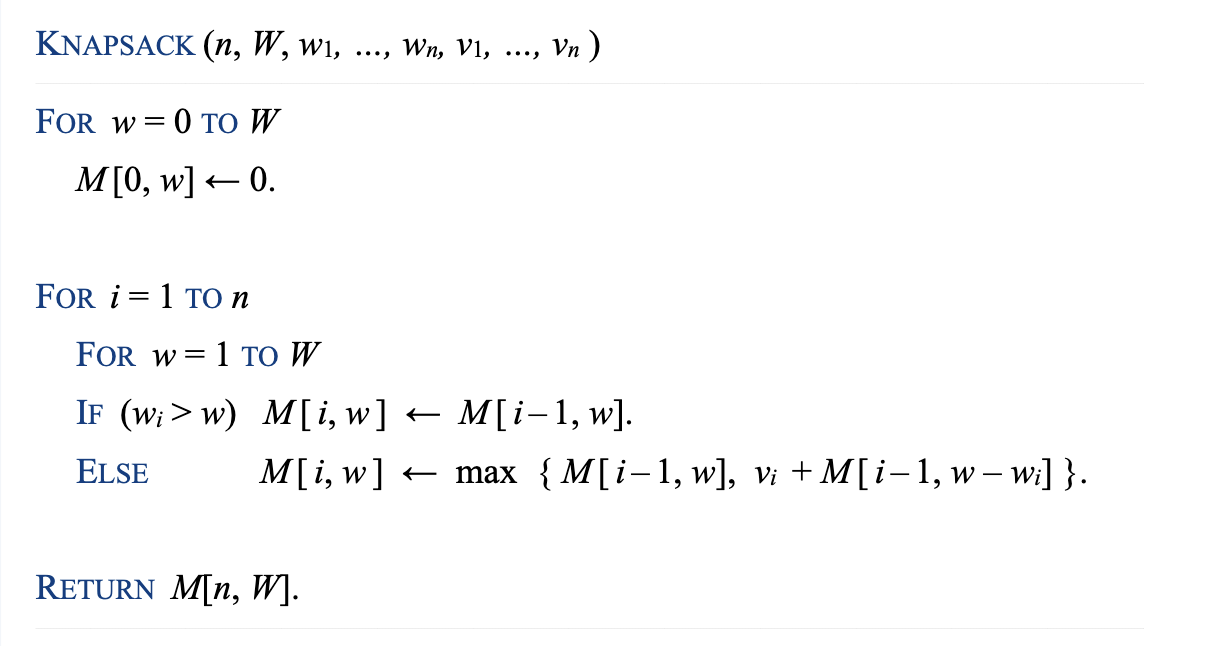
\includegraphics[width=0.9\textwidth]{imm/Screenshot 2026-03-16 alle 08.49.41.png}
\end{figure}

\textbf{Tracing the solution.} After computing the table, item $i$ is in the optimal solution
for $(i, w)$ if and only if $M[i, w] > M[i-1, w]$.
\begin{figure}[H]
\centering
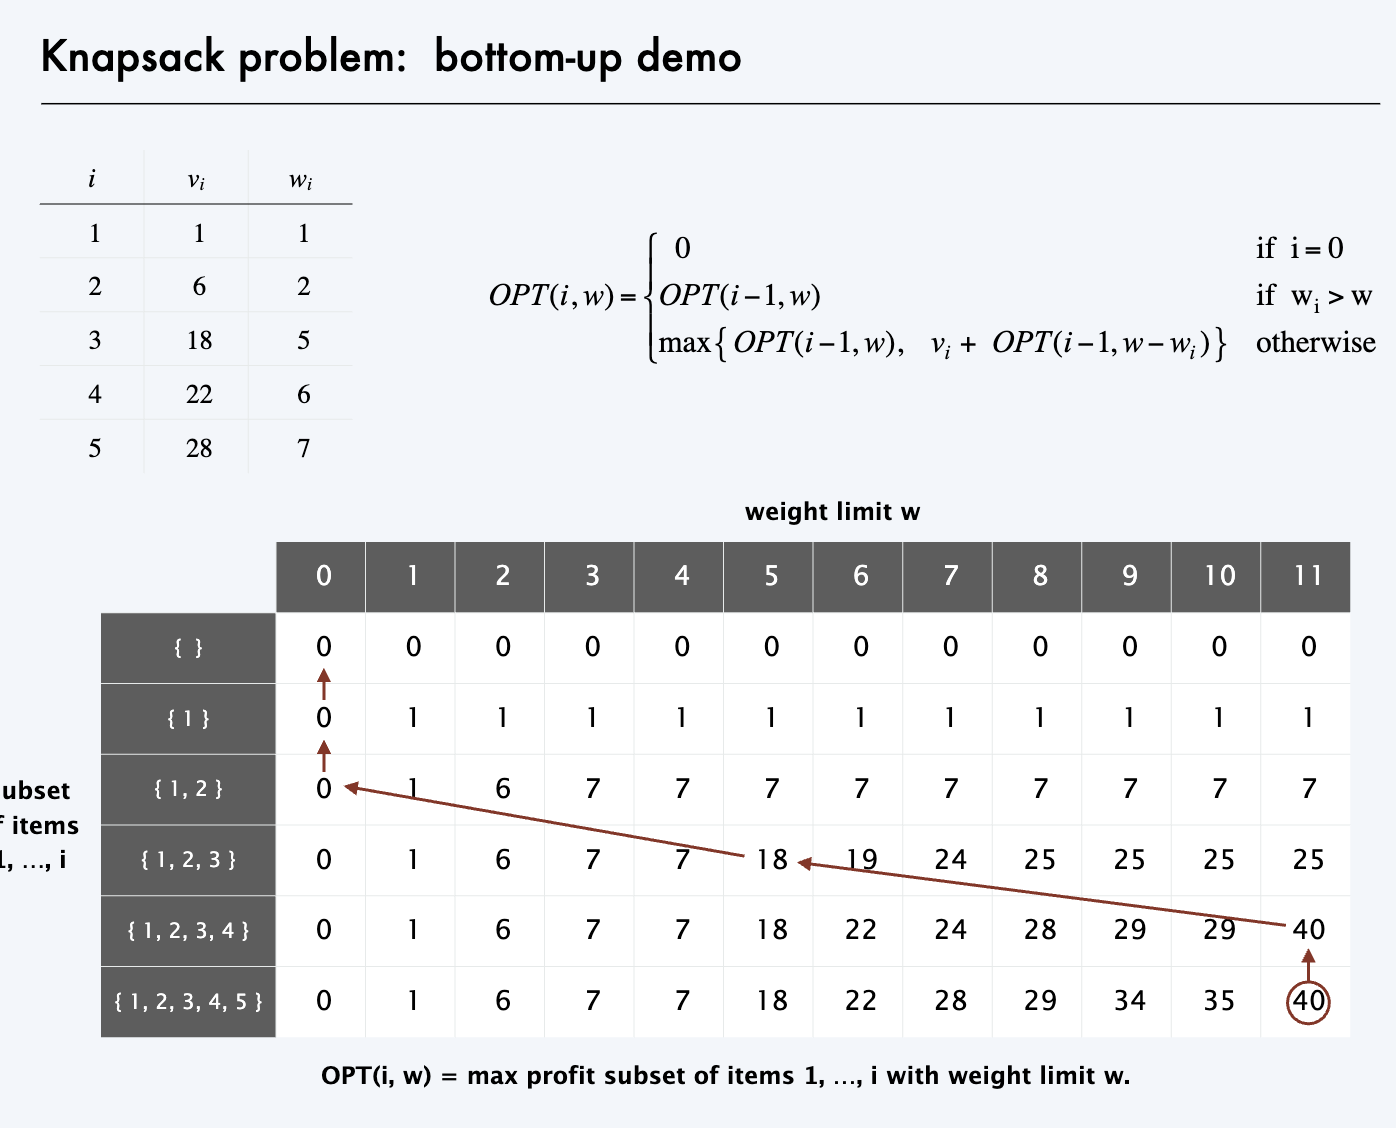
\includegraphics[width=0.9\textwidth]{imm/Screenshot 2026-03-16 alle 08.55.17.png}
\end{figure}
\subsection{Running Time and Remarks}

\begin{theorem}
The knapsack DP algorithm runs in $\Theta(nW)$ time and $\Theta(nW)$ space.
\end{theorem}

\begin{proof}
Each of the $\Theta(nW)$ table entries is filled in $O(1)$ time.
\end{proof}

\textbf{Important remark.} The running time $\Theta(nW)$ is \emph{not} polynomial in the
input size. The input size is $O(n \log W)$ (since $W$ is encoded in binary), so the
algorithm is \textbf{pseudo-polynomial}. In fact:
\begin{itemize}
    \item The decision version of knapsack is \textbf{NP-complete} (Chapter 8).
    \item There exists a polynomial-time approximation scheme (PTAS) that finds a solution
    within 1\% of the optimum (Section 11.8).
\end{itemize}
in particular:
\begin{math}
    if(v_i<V-- w_i<W)
    \newline
   I(n, w)=  \sum_{i=1}^{n} log w_i + log v_i + log W =
   = O(n * max(log W, log V))
   =O(n log W)
\end{math}


%────────────────────────────────────────────────────────────
\section{Sequence Alignment}

\subsection{String Similarity and Edit Distance}

A natural question in computer science and biology is: \emph{how similar are two strings?}
Consider the strings \texttt{ocurrance} and \texttt{occurrence}. Depending on how we align
them, we get very different costs:
\begin{figure}[H]
\centering
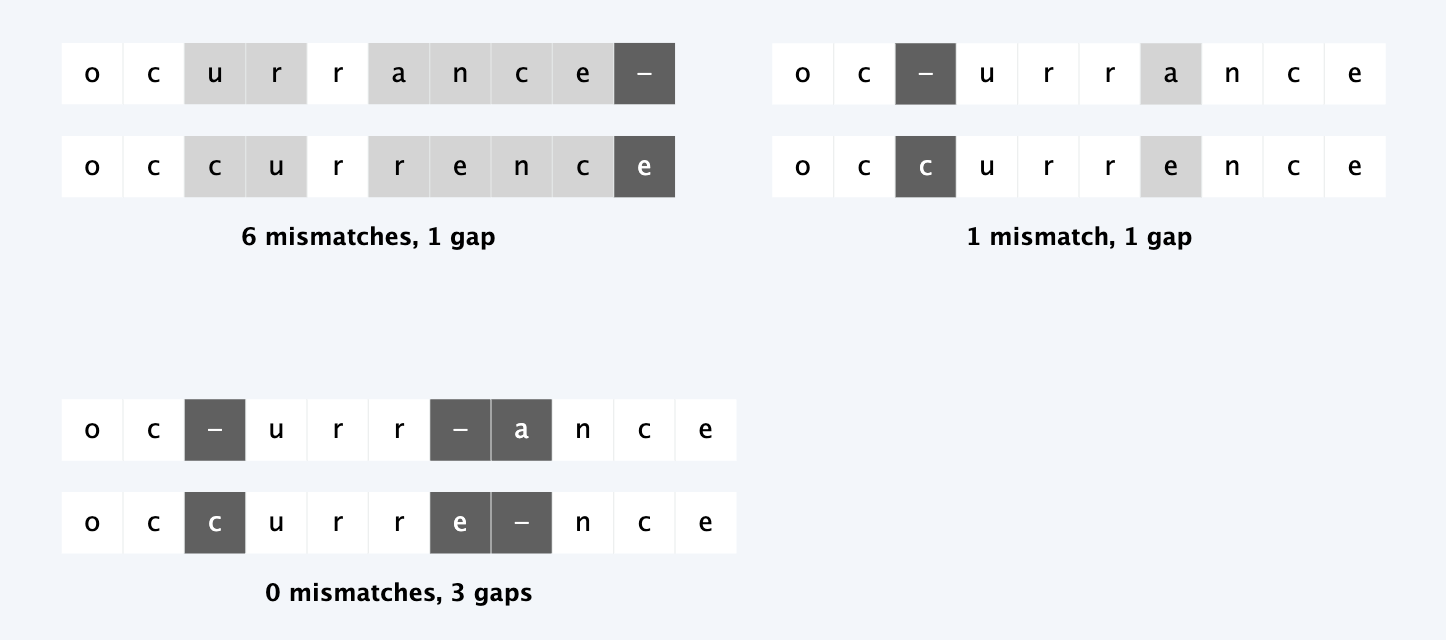
\includegraphics[width=0.7\textwidth]{imm/Screenshot 2026-03-16 alle 09.58.55.png}
\end{figure}
The \textbf{edit distance} (Levenshtein 1966, Needleman--Wunsch 1970) measures this cost
formally using two parameters:
\begin{itemize}
    \item $\delta$ = gap penalty (cost of leaving a character unmatched)
    \item $\alpha_{pq}$ = mismatch penalty for aligning character $p$ with character $q$
    (equals 0 if $p = q$)
\end{itemize}
\begin{figure}[H]
\centering
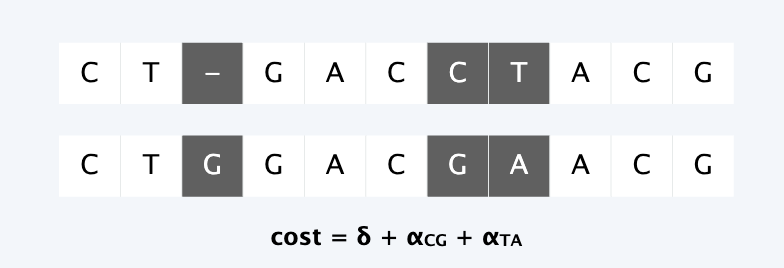
\includegraphics[width=0.5\textwidth]{imm/Screenshot 2026-03-16 alle 10.03.50.png}
\end{figure}
\textbf{Applications:} Unix \texttt{diff}, spell checking, speech recognition, computational
biology (DNA/protein alignment), and more.

\subsection{Problem Definition}

\begin{definition}[Alignment]
Given strings $x_1 x_2 \ldots x_m$ and $y_1 y_2 \ldots y_n$, an \emph{alignment} $M$ is a
set of ordered pairs $(x_i, y_j)$ such that each character appears in at most one pair, and
there are no \emph{crossings} (i.e., if $(x_i, y_j) \in M$ and $(x_{i'}, y_{j'}) \in M$
with $i < i'$, then $j < j'$).
\end{definition}

\begin{definition}[Cost of an alignment]
\[
    \text{cost}(M) =
    \underbrace{\sum_{(x_i, y_j) \in M} \alpha_{x_i y_j}}_{\text{mismatch}}
    + \underbrace{\delta \sum_{i:\, x_i \text{ unmatched}} 1
    + \delta \sum_{j:\, y_j \text{ unmatched}} 1}_{\text{gaps}}
\]
\end{definition}

\textbf{Goal.} Find the alignment of minimum cost.
\begin{figure}[H]
\centering
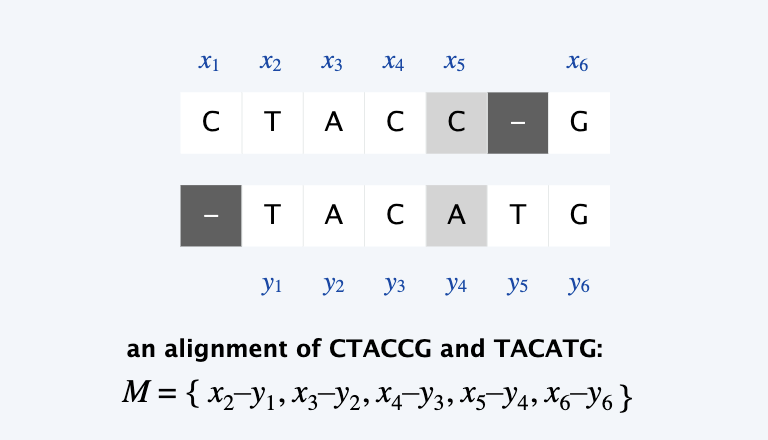
\includegraphics[width=0.5\textwidth]{imm/Screenshot 2026-03-16 alle 10.11.11.png}
\end{figure}
\subsection{Optimal Substructure}

\begin{definition}
$\text{OPT}(i, j)$ = minimum cost of aligning the prefix strings $x_1 \ldots x_i$ and
$y_1 \ldots y_j$.
\end{definition}

There are three cases for what happens to the last characters $x_i$ and $y_j$:
\begin{enumerate}
    \item \textbf{$x_i$ is matched with $y_j$:} pay mismatch $\alpha_{x_i y_j}$, then
    solve the subproblem on $x_1 \ldots x_{i-1}$ and $y_1 \ldots y_{j-1}$.
    \item \textbf{$x_i$ is left unmatched (gap):} pay $\delta$, then solve on
    $x_1 \ldots x_{i-1}$ and $y_1 \ldots y_j$.
    \item \textbf{$y_j$ is left unmatched (gap):} pay $\delta$, then solve on
    $x_1 \ldots x_i$ and $y_1 \ldots y_{j-1}$.
\end{enumerate}

This gives the recurrence:
\[
    \text{OPT}(i, j) =
    \begin{cases}
        j \delta & \text{if } i = 0 \\
        i \delta & \text{if } j = 0 \\
        \min \left\{
            \alpha_{x_i y_j} + \text{OPT}(i-1, j-1),\;
            \delta + \text{OPT}(i-1, j),\;
            \delta + \text{OPT}(i, j-1)
        \right\} & \text{otherwise}
    \end{cases}
\]
in the first two cases, we have to pay a gap penalty for each unmatched character because one of the 2 strings is empty. In the third case, we have a \textbf{three-way choice}: we can match $x_i$ with $y_j$, or leave $x_i$ unmatched, or leave $y_j$ unmatched.
\subsection{Algorithm}

\begin{figure}[H]
\centering
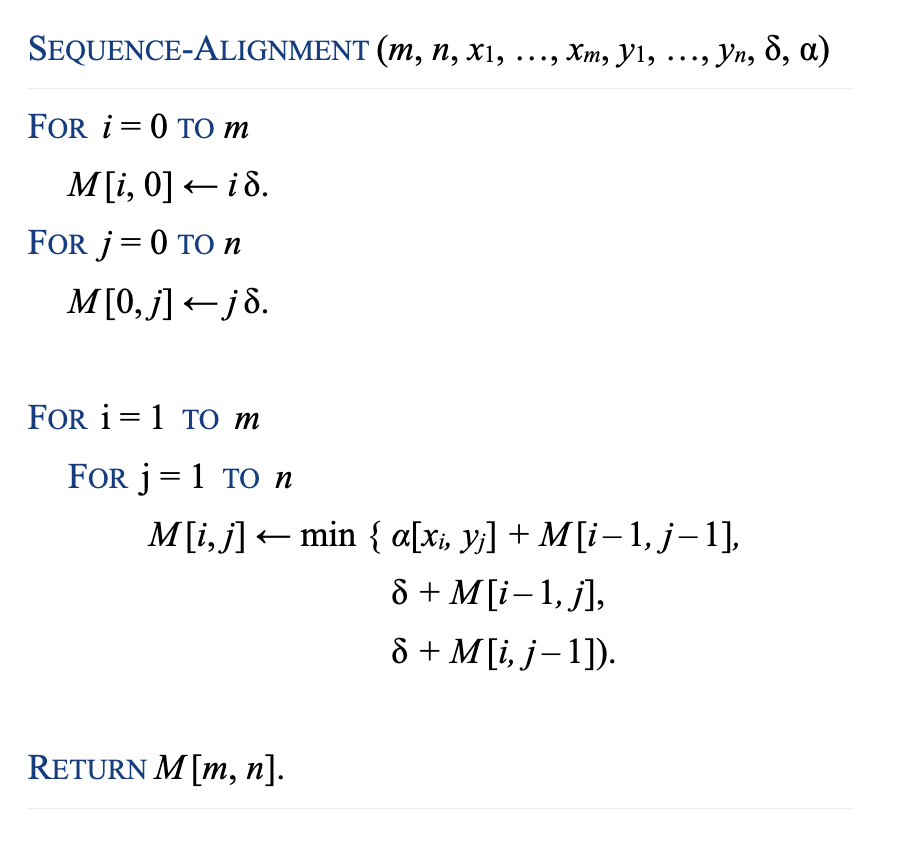
\includegraphics[width=0.9\textwidth]{imm/Screenshot 2026-03-16 alle 10.16.56.png}
\end{figure}

\begin{theorem}
The DP algorithm computes the edit distance of two strings of length $m$ and $n$ in
$\Theta(mn)$ time and $\Theta(mn)$ space.
\end{theorem}

\textbf{Recovering the alignment.} To find not just the cost but also the actual alignment,
trace back through the DP table from $M[m, n]$ to $M[0, 0]$, following the choice that was
made at each step.

\textbf{Space optimisation.} We can compute the optimal \emph{value} in $O(mn)$ time and
only $O(m + n)$ space by keeping just two rows of the table at a time. However, this makes
it hard to recover the actual alignment.

% ─────────────────────────────────────────────
\section{Hirschberg's Algorithm}

\subsection{Goal: Linear Space with Full Alignment}

\begin{theorem}
There exists an algorithm to find an optimal alignment in $O(mn)$ time and $O(m + n)$ space.
\end{theorem}

This is achieved by a clever combination of divide-and-conquer and dynamic programming
(Hirschberg, 1975). The key insight is to model the problem as a shortest-path problem.

\subsection*{Edit Distance Graph}
\begin{figure}[H]
\centering
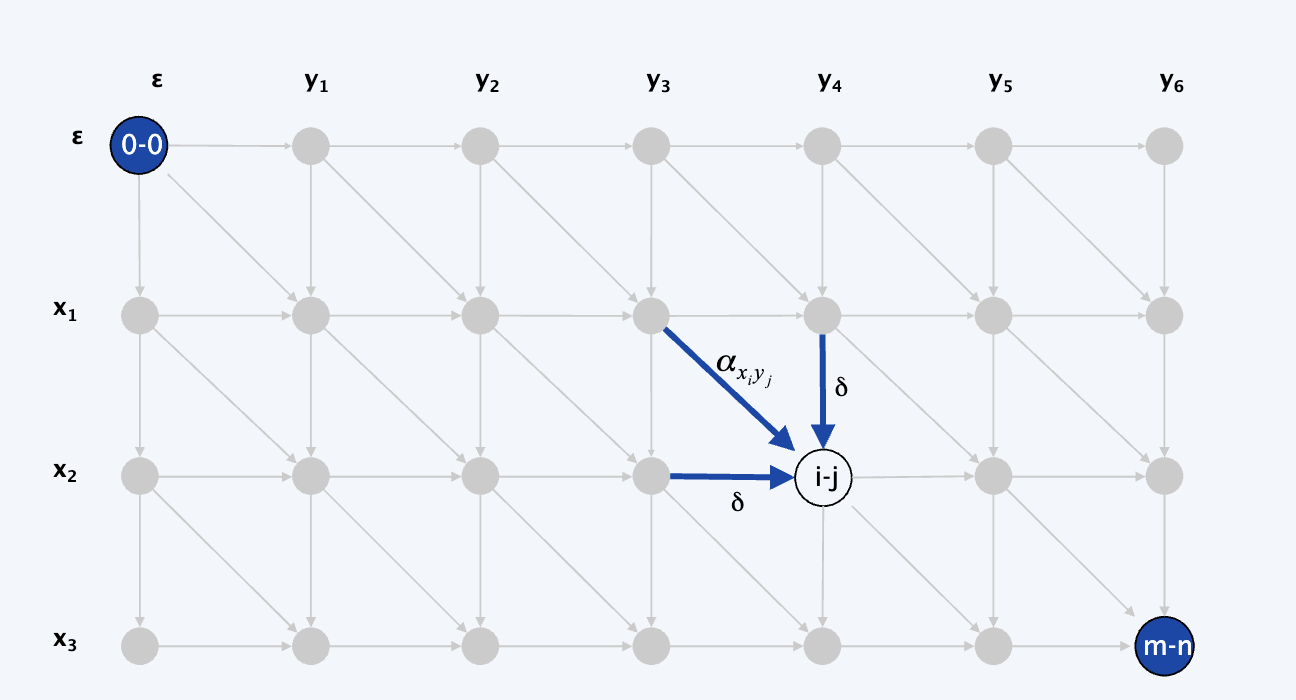
\includegraphics[width=0.9\textwidth]{imm/Screenshot 2026-03-16 alle 10.24.13.png}
\caption{The edit distance problem can be represented as a shortest path problem in a directed acyclic graph. Each node corresponds to a pair of indices $(i, j)$, and edges represent the three possible operations (match/mismatch(diagonale), gap in $x$, gap in $y$(verticale/orizzontale)) with their associated costs. The optimal alignment corresponds to the shortest path from $(0, 0)$ to $(m, n)$.}
\end{figure}
\begin{lemma}
Let $f(i, j)$ be the cost of the shortest path from $(0,0)$ to $(i, j)$. Then
$f(i, j) = \text{OPT}(i, j)$ for all $i, j$.
\end{lemma}

\begin{proof}[Proof (by strong induction on $i + j$)]
Base case: $f(0,0) = \text{OPT}(0,0) = 0$.
Inductive step: the last edge into $(i, j)$ comes from $(i{-}1, j{-}1)$, $(i{-}1, j)$,
or $(i, j{-}1)$. Applying the inductive hypothesis to each predecessor:
\[
    f(i, j) = \min\{
        \alpha_{x_i y_j} + f(i{-}1, j{-}1),\;
        \delta + f(i{-}1, j),\;
        \delta + f(i, j{-}1)
    \} = \text{OPT}(i, j). \qquad \square
\]
\end{proof}

\subsection*{Forward and Backward Distances}

Define two functions:
\begin{itemize}
    \item $f(i, j)$ = shortest path from $(0,0)$ to $(i, j)$ (computed \emph{forward}).
    \item $g(i, j)$ = shortest path from $(i, j)$ to $(m, n)$ (computed \emph{backward},
    by reversing all edges and swapping the roles of $(0,0)$ and $(m,n)$).
\end{itemize}

Both $f(\cdot, j)$ and $g(\cdot, j)$ can be computed for any fixed column $j$ in
$O(mn)$ time and $O(m + n)$ space.
\begin{figure}[H]
\centering
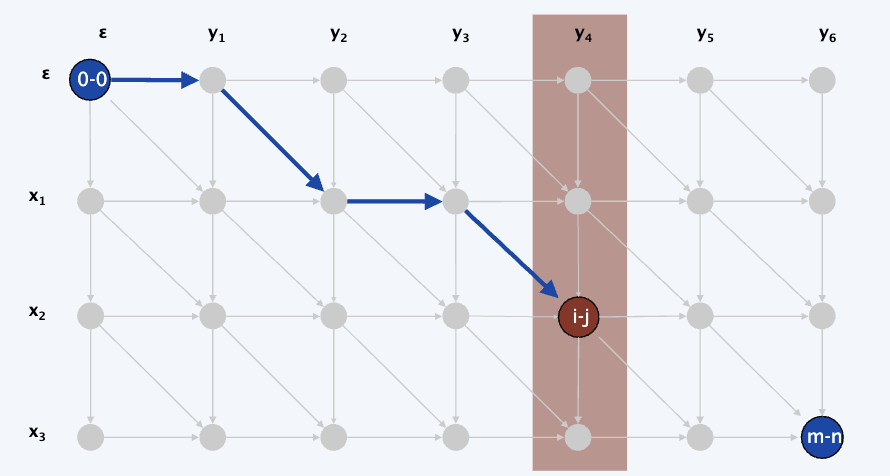
\includegraphics[width=0.6\textwidth]{imm/Screenshot 2026-04-14 alle 13.46.24.png}
\end{figure}

\textbf{Key observations:}
\begin{enumerate}
    \item The total cost of the shortest path through node $(i, j)$ is $f(i, j) + g(i, j)$.
    \item Let $q$ be the index that minimises $f(q, \lfloor n/2 \rfloor) + g(q, \lfloor n/2 \rfloor)$.
    Then the optimal alignment passes through node $(q, \lfloor n/2 \rfloor)$.
\end{enumerate}
In other words, the optimal alignment is not just any path through the graph: it must pass through a specific node in the middle column. This key observation makes the divide-and-conquer approach possible, because it guarantees that some node in the middle column belongs to the optimal solution, and we can identify it by combining the forward and backward dynamic programming computations.
\subsection{Divide-and-Conquer}

\begin{enumerate}
    \item \textbf{Divide.} Compute $f(\cdot, n/2)$ (forward) and $g(\cdot, n/2)$ (backward).
    Find index $q$ minimising $f(q, n/2) + g(q, n/2)$. The optimal alignment passes through
    $(q, n/2)$.
    \item \textbf{Conquer.} Recursively compute the optimal alignment in:
    \begin{itemize}
        \item the top-left subproblem: $x_1 \ldots x_q$ vs.\ $y_1 \ldots y_{n/2}$
        \item the bottom-right subproblem: $x_{q+1} \ldots x_m$ vs.\ $y_{n/2+1} \ldots y_n$
    \end{itemize}
\end{enumerate}
\begin{figure}[H]
\centering
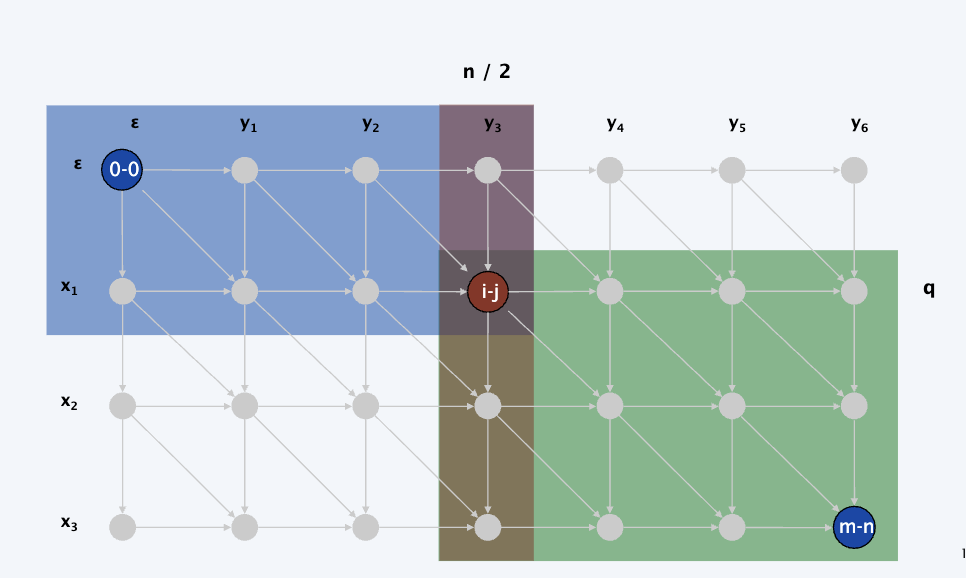
\includegraphics[width=0.6\textwidth]{imm/Screenshot 2026-04-14 alle 13.52.49.png}
\end{figure}
\subsubsection*{Example of Hirschberg's Algorithm}

Consider the strings $x = \texttt{AC}$ and $y = \texttt{AGC}$.

The goal is to find an optimal alignment between these two strings. Hirschberg's algorithm first splits the second string in the middle. Since $y$ has length 3, the middle column is $\lfloor 3/2 \rfloor = 1$, so we look at the first character \texttt{A}.

Now we do two computations:
\begin{itemize}
    \item a forward computation from the start to the middle column,
    \item a backward computation from the end to the middle column.
\end{itemize}

For each possible row $q$, we add the forward cost and the backward cost. The best value tells us which node in the middle column belongs to the optimal alignment.

In this example, the best path passes through the node that matches the first \texttt{A}. After that, the problem is split into two smaller parts:
\begin{itemize}
    \item the left part, before the middle column,
    \item the right part, after the middle column.
\end{itemize}

This example shows the main idea of Hirschberg's algorithm: find one correct point in the middle, then solve the two halves recursively. The final result is the same optimal alignment as the standard dynamic programming algorithm, but with much less space.
\subsection{Running Time Analysis}

\begin{theorem}
Hirschberg's algorithm runs in $O(mn)$ time and $O(m + n)$ space.
\end{theorem}

\begin{proof}[Proof (by induction on $n$)]
Let $T(m, n)$ be the running time. The divide step takes $O(mn)$ time. The two subproblems
are of sizes $(q, n/2)$ and $(m - q, n/2)$. Choose constant $c$ such that the divide step
costs at most $cmn$. Claim: $T(m, n) \leq 2cmn$.
\begin{align*}
    T(m, n) &\leq T(q, n/2) + T(m - q, n/2) + cmn \\
            &\leq 2cq(n/2) + 2c(m - q)(n/2) + cmn \\
            &= cqn + cmn - cqn + cmn \\
            &= 2cmn. \qquad \square
\end{align*}
The key point is that the two subproblems split the \emph{rows} ($q$ and $m - q$), so the
total work across all levels of recursion stays $O(mn)$.
\end{proof}

% ─────────────────────────────────────────────
\section{Bellman-Ford Algorithm}

\subsection{The Shortest Path Problem with Negative Weights}

\textbf{Problem.} Given a directed graph $G = (V, E)$ with arbitrary edge weights $c_{vw}$,
find the cheapest path from every node $v$ to a destination node $t$.
\begin{figure}[H]
\centering
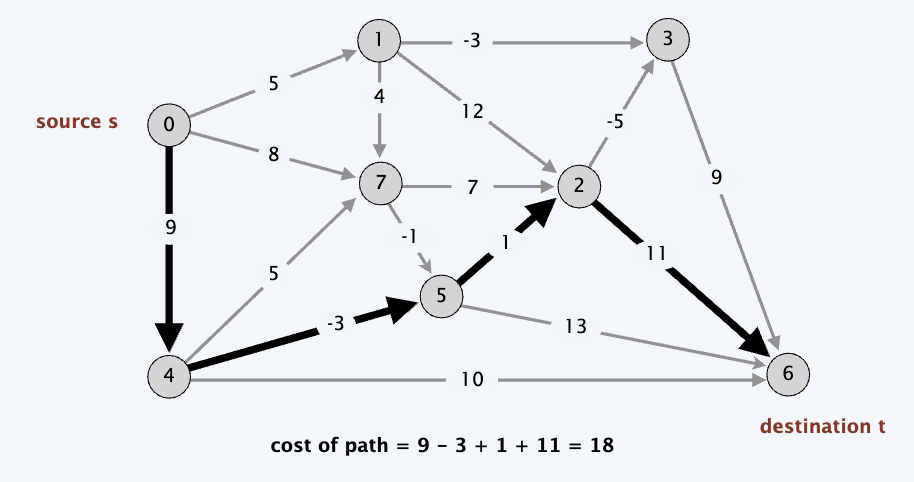
\includegraphics[width=0.6\textwidth]{imm/Screenshot 2026-04-14 alle 14.08.28.png}
\end{figure}
\textbf{Why Dijkstra fails.} Dijkstra's algorithm requires non-negative edge weights. With
negative weights it can give wrong answers. A simple fix (adding a constant to all edges) also
fails because it changes the lengths of paths with different numbers of edges.

\subsection{Negative Cycles}

\begin{definition}[Negative cycle]
A \emph{negative cycle} is a directed cycle $W$ such that $\sum_{e \in W} c_e < 0$.
\end{definition}
\begin{figure}[H]
\centering
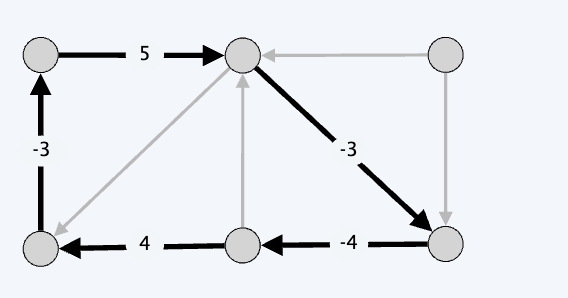
\includegraphics[width=0.4\textwidth]{imm/Screenshot 2026-04-14 alle 14.10.03.png}
\end{figure}
\begin{lemma}
If some path from $v$ to $t$ contains a negative cycle, then there is no cheapest path from
$v$ to $t$ (the cost can be made arbitrarily negative).
\end{lemma}

\begin{lemma}
If $G$ has no negative cycles, then there exists a cheapest $v \leadsto t$ path that is
simple (uses at most $n - 1$ edges).
\end{lemma}

\begin{proof}
Take a cheapest path with the fewest edges. If it contains a cycle $W$, removing $W$ gives
a cheaper or equal-cost path with fewer edges (since $c(W) \geq 0$). Contradiction.
\end{proof}
\subsubsection*{Shortest path and negative cycle problems}
\begin{itemize}
    \item Shortest path problem. Given a digraph G = (V, E) with edge weights cvw and no negative cycles, find cheapest v to t path for each node v.
    \item Negative cycle problem. Given a digraph G = (V, E) with edge weights cvw, determine
whether G contains a negative cycle.
\end{itemize}
The two problems are closely related: if we can solve the shortest path problem, we can check for negative cycles by seeing if any path cost can be reduced by going around a cycle. Conversely,if we can solve the negative cycle problem, we can find shortest paths by first checking for negative cycles and then applying a shortest path algorithm that assumes no negative cycles.
\subsection{Dynamic Programming Formulation}

\begin{definition}
$\text{OPT}(i, v)$ = cost of the cheapest $v \leadsto t$ path using at most $i$ edges.
\end{definition}

\textbf{Recurrence:}
(è come se partissi da t e facessi passi indietro, ogni passo indietro può essere o restare fermi o prendere un arco in ingresso)
\[
    \text{OPT}(i, v) =
    \begin{cases}
        0 & \text{if } i = 0 \text{ and } v = t \\
        \infty & \text{if } i = 0 \text{ and } v \neq t \\
        \min\!\left\{
            \text{OPT}(i-1, v),\;
            \min_{(v,w) \in E}\bigl\{\text{OPT}(i-1, w) + c_{vw}\bigr\}
        \right\} & \text{otherwise}
    \end{cases}
\]

The two cases are: (1) the cheapest path uses $\leq i - 1$ edges (do not move yet), or (2) it
uses exactly $i$ edges (take the first edge $(v, w)$ and then find the best $w \leadsto t$
path with $\leq i - 1$ edges).

\textbf{Key observation.} If $G$ has no negative cycles, then $\text{OPT}(n-1, v)$ gives
the cost of the cheapest $v \leadsto t$ path (by Lemma 2, the cheapest path is simple and has
at most $n - 1$ edges).

\subsection{Implementation}

\begin{lstlisting}[language=Python]
SHORTEST-PATHS(V, E, c, t)
  FOR each node v in V:
      M[0, v] = infinity
  M[0, t] = 0
  FOR i = 1 TO n-1:
      FOR each node v in V:
          M[i, v] = M[i-1, v]
          FOR each edge (v, w) in E:
              M[i, v] = min(M[i, v], M[i-1, w] + c(v,w))
  RETURN M
\end{lstlisting}

\begin{theorem}
Given a digraph with no negative cycles, the DP algorithm computes the cost of the cheapest
$v \leadsto t$ path for each node $v$ in $\Theta(mn)$ time and $\Theta(n^2)$ space.
\end{theorem}

\subsection{Bellman-Ford: Efficient Implementation}

In practice, we use only $O(n)$ space by maintaining a single array $d(v)$ (the best distance
found so far) and a successor pointer.

\begin{lstlisting}[language=Python]
BELLMAN-FORD(V, E, c, t)
  FOR each node v in V:
      d(v) = infinity
      successor(v) = null
  d(t) = 0
  FOR i = 1 TO n-1:
      FOR each node w in V:
          IF d(w) was updated in previous iteration:
              FOR each edge (v, w) in E:
                  IF d(v) > d(w) + c(v,w):
                      d(v) = d(w) + c(v,w)
                      successor(v) = w
      IF no d(w) value changed in this iteration: STOP
\end{lstlisting}

\textbf{Performance optimisation.} If $d(w)$ was not updated in iteration $i - 1$, there is
no reason to consider edges entering $w$ in iteration $i$. This can make the algorithm much
faster in practice.

\subsection{Analysis and Correctness}

\begin{lemma}
Throughout Bellman-Ford, $d(v)$ is the cost of \emph{some} $v \leadsto t$ path. After pass
$i$, $d(v) \leq \text{OPT}(i, v)$.
\end{lemma}

\begin{proof}[Proof (by induction on $i$)]
After pass $i+1$, for any $v \leadsto t$ path $P$ with $i+1$ edges, let $(v, w)$ be the
first edge and $P'$ be the subpath from $w$ to $t$. By the inductive hypothesis,
$d(w) \leq c(P')$. After considering $v$ in pass $i+1$:
\[
    d(v) \leq c_{vw} + d(w) \leq c_{vw} + c(P') = c(P). \qquad \square
\]
\end{proof}

\begin{theorem}
Given a digraph with no negative cycles, Bellman-Ford computes the costs of the cheapest
$v \leadsto t$ paths in $O(mn)$ time and $\Theta(n)$ extra space.
\end{theorem}

\textbf{Caution.} The claim that ``following successor pointers always gives a path of cost
$d(v)$'' is \emph{false} in general during the algorithm (the successor graph may contain
cycles or have inconsistent costs). However, upon termination with no negative cycles, the
successor graph is a tree and following pointers from any $s$ gives the correct shortest path.

\begin{lemma}
If the successor graph contains a directed cycle $W$ at any point during Bellman-Ford, then
$W$ is a negative cycle.
\end{lemma}

\begin{proof}
When \texttt{successor(v) = w} is set, we have $d(v) \geq d(w) + c_{vw}$. Let
$v_1 \to v_2 \to \cdots \to v_k \to v_1$ be the cycle. Summing the inequalities (with a strict
inequality for the last edge added to the cycle) gives:
\[
    c(v_1, v_2) + c(v_2, v_3) + \cdots + c(v_k, v_1) < 0. \qquad \square
\]
\end{proof}

\begin{theorem}
Given a digraph with no negative cycles, Bellman-Ford finds the cheapest $s \leadsto t$ paths
in $O(mn)$ time and $\Theta(n)$ extra space.
\end{theorem}

\begin{proof}
By Lemma 4, the successor graph has no cycle on termination. Following successor pointers from
$s$ gives a path $s = v_1 \to v_2 \to \cdots \to v_k = t$. Upon termination, for each
$\texttt{successor}(v) = w$, we have $d(v) = d(w) + c_{vw}$ (since values no longer change).
Summing along the path: $d(s) = d(t) + \sum_{\text{edges}} c = c(P)$. Combined with Theorem 2,
$c(P)$ is the minimum cost. \qquad$\square$
\end{proof}

% ─────────────────────────────────────────────
\section{Distance Vector Protocols}

\subsection{Routing in Communication Networks}

In a communication network, nodes are routers, edges are direct links, and edge weights
represent link delays. We want each router to know the shortest path to every other router.

\textbf{Dijkstra} needs global knowledge of the whole network. \textbf{Bellman-Ford} needs
only local knowledge of neighbouring nodes — each router only talks to its neighbours.

\subsection{Distance Vector Protocols}

Each router maintains:
\begin{itemize}
    \item A vector of shortest known distances to every other node.
    \item The first hop (direction) on each shortest path.
\end{itemize}

The algorithm runs $n$ separate Bellman-Ford computations, one for each destination.
Updates propagate through the network by \emph{``routing by rumour''}: each router shares
its distance vector with its neighbours, and they update their own vectors accordingly.

\textbf{Examples:} RIP, Cisco's IGRP, AppleTalk's RTMP, Novell's IPX RIP.

\textbf{Asynchrony.} The algorithm still converges even if routers do not update in lockstep.

\subsection{Counting-to-Infinity Problem}

\textbf{Problem.} If a link is deleted, distance vector protocols can get stuck in a loop
where routers keep increasing their estimated distances, very slowly converging.

\textbf{Example.} If the link $s \to t$ (cost 1) is deleted, $s$ thinks it can reach $t$
via $v$ (cost 2), then $v$ updates via $s$ (cost 3), and so on — slowly counting to infinity.

\subsection{Path Vector Protocols}

\textbf{Link-state routing} fixes the counting-to-infinity problem by storing the full path
(not just the distance and first hop). This allows routers to detect loops immediately.
Requires much more storage. Used in \textbf{BGP} (internet routing) and \textbf{OSPF}.

% ─────────────────────────────────────────────
\section{Negative Cycle Detection}

\subsection{The Problem}

\textbf{Goal.} Given a directed graph $G = (V, E)$ with edge weights $c_{vw}$, find a
negative cycle if one exists.

\textbf{Application: Currency Arbitrage.} Given $n$ currencies and exchange rates between
pairs, is there a sequence of conversions that makes a profit?

\textbf{Example.} USD $\to$ EUR $\to$ GBP $\to$ USD with rates $0.741 \times 1.366 \times
0.995 = 1.00714 > 1$: this is an arbitrage opportunity. Modelling this as a graph problem
(with $-\log(\text{exchange rate})$ as edge weights), arbitrage corresponds to a negative
cycle.

\subsection{Detection via Bellman-Ford}

\begin{lemma}
If $\text{OPT}(n, v) = \text{OPT}(n-1, v)$ for all $v$, then there is no negative cycle.
\end{lemma}

\begin{lemma}
If $\text{OPT}(n, v) < \text{OPT}(n-1, v)$ for some node $v$, then the cheapest $v \leadsto t$
path has exactly $n$ edges. By the pigeonhole principle, it contains a directed cycle $W$.
Since removing $W$ would give a shorter path, $W$ must be a negative cycle.
\end{lemma}

\subsection{Algorithm}

\begin{theorem}
A negative cycle can be found in $\Theta(mn)$ time and $\Theta(n^2)$ space.
\end{theorem}

\begin{proof}
Add a new node $t$ and connect every node to $t$ with a 0-cost edge. The new graph $G'$ has
a negative cycle if and only if $G$ has one. Run the DP for $n$ iterations (instead of $n-1$).
If $\text{OPT}(n, v) = \text{OPT}(n-1, v)$ for all $v$: no negative cycle. Otherwise,
extract the directed cycle from the path from $v$ to $t$ (the cycle cannot contain $t$ since
no edges leave $t$).
\end{proof}

\begin{theorem}
A negative cycle can be found in $O(mn)$ time and $O(n)$ extra space.
\end{theorem}

\begin{proof}
Run Bellman-Ford for $n$ passes (not $n-1$) on the modified digraph $G'$.
\begin{itemize}
    \item If no $d(v)$ is updated in pass $n$: no negative cycle.
    \item Otherwise, suppose $d(s)$ is updated in pass $n$. Define
    $\text{pass}(v)$ = last pass in which $d(v)$ was updated. We have
    $\text{pass}(s) = n$ and $\text{pass}(\text{successor}(v)) \geq \text{pass}(v) - 1$.
    Following successor pointers from $s$, we must eventually revisit a node. By Lemma 4,
    the resulting cycle is a negative cycle. \qquad$\square$
\end{itemize}
\end{proof}

\subsection{Summary of Complexities}

\begin{center}
\begin{tabular}{@{}llll@{}}
\toprule
\textbf{Algorithm} & \textbf{Problem} & \textbf{Time} & \textbf{Space} \\
\midrule
Sequence Alignment (basic DP) & Edit distance + alignment & $\Theta(mn)$ & $\Theta(mn)$ \\
Sequence Alignment (space opt.) & Edit distance only & $O(mn)$ & $O(m+n)$ \\
Hirschberg's algorithm & Edit distance + alignment & $O(mn)$ & $O(m+n)$ \\
Shortest Paths (basic DP) & No negative cycles & $\Theta(mn)$ & $\Theta(n^2)$ \\
Bellman-Ford (efficient) & No negative cycles & $O(mn)$ & $\Theta(n)$ \\
Negative Cycle Detection & Find neg. cycle & $\Theta(mn)$ / $O(mn)$ & $\Theta(n^2)$ / $O(n)$ \\
\bottomrule
\end{tabular}
\end{center}

\chapter{ exercises on dynamic programming}
\textbf{Problem 1 (Max Independent Set on Line Graphs)}

Let $G = (V,E)$ be a line graph of $n$ nodes formed by a sequence of nodes
$v_1, v_2, \ldots, v_n$ with an edge between $v_i$ and $v_j$ if and only if
$i$ and $j$ differs by exactly $1$. With every vertex $i$, we associate a
positive integer weight $w_i$. Recall that a set of nodes is an
\emph{independent set} if no two nodes of them are joined by an edge.
The goal is to find an independent set of $G$ of maximum total weight.

\begin{enumerate}
  \item[(a)] Show on an example that a greedy strategy fails to find an optimal solution.
  \item[(b)] Give an algorithm that finds an independent set of maximum total
            weight in time which is polynomial in the number of vertices and
            it does not depend from the weights of the nodes.
  \item[(c)] Provide the pseudo-code of an efficient implementation of the
            algorithm and discuss its time and space complexity.
\end{enumerate}
\textbf{solution}
\begin{enumerate}
  \item[(a)] the greedy strategy fails to find an optimal solution. For example, consider the line graph with 7 nodes and weights 
  $w_1 = 9$, $w_2 = 10$, $w_3 = 9$, $w_4 = 0$, $w_5 = 9$, $w_6 = 10$, $w_7 = 9$.
The greedy strategy would pick the greater value so it would pick $v_2$ and $v_6$ with total weight $20$. However, the optimal solution is to pick $v_1$, $v_3$, $v_5$, and $v_7$ with total weight $36$.
\begin{figure}[H]
\centering
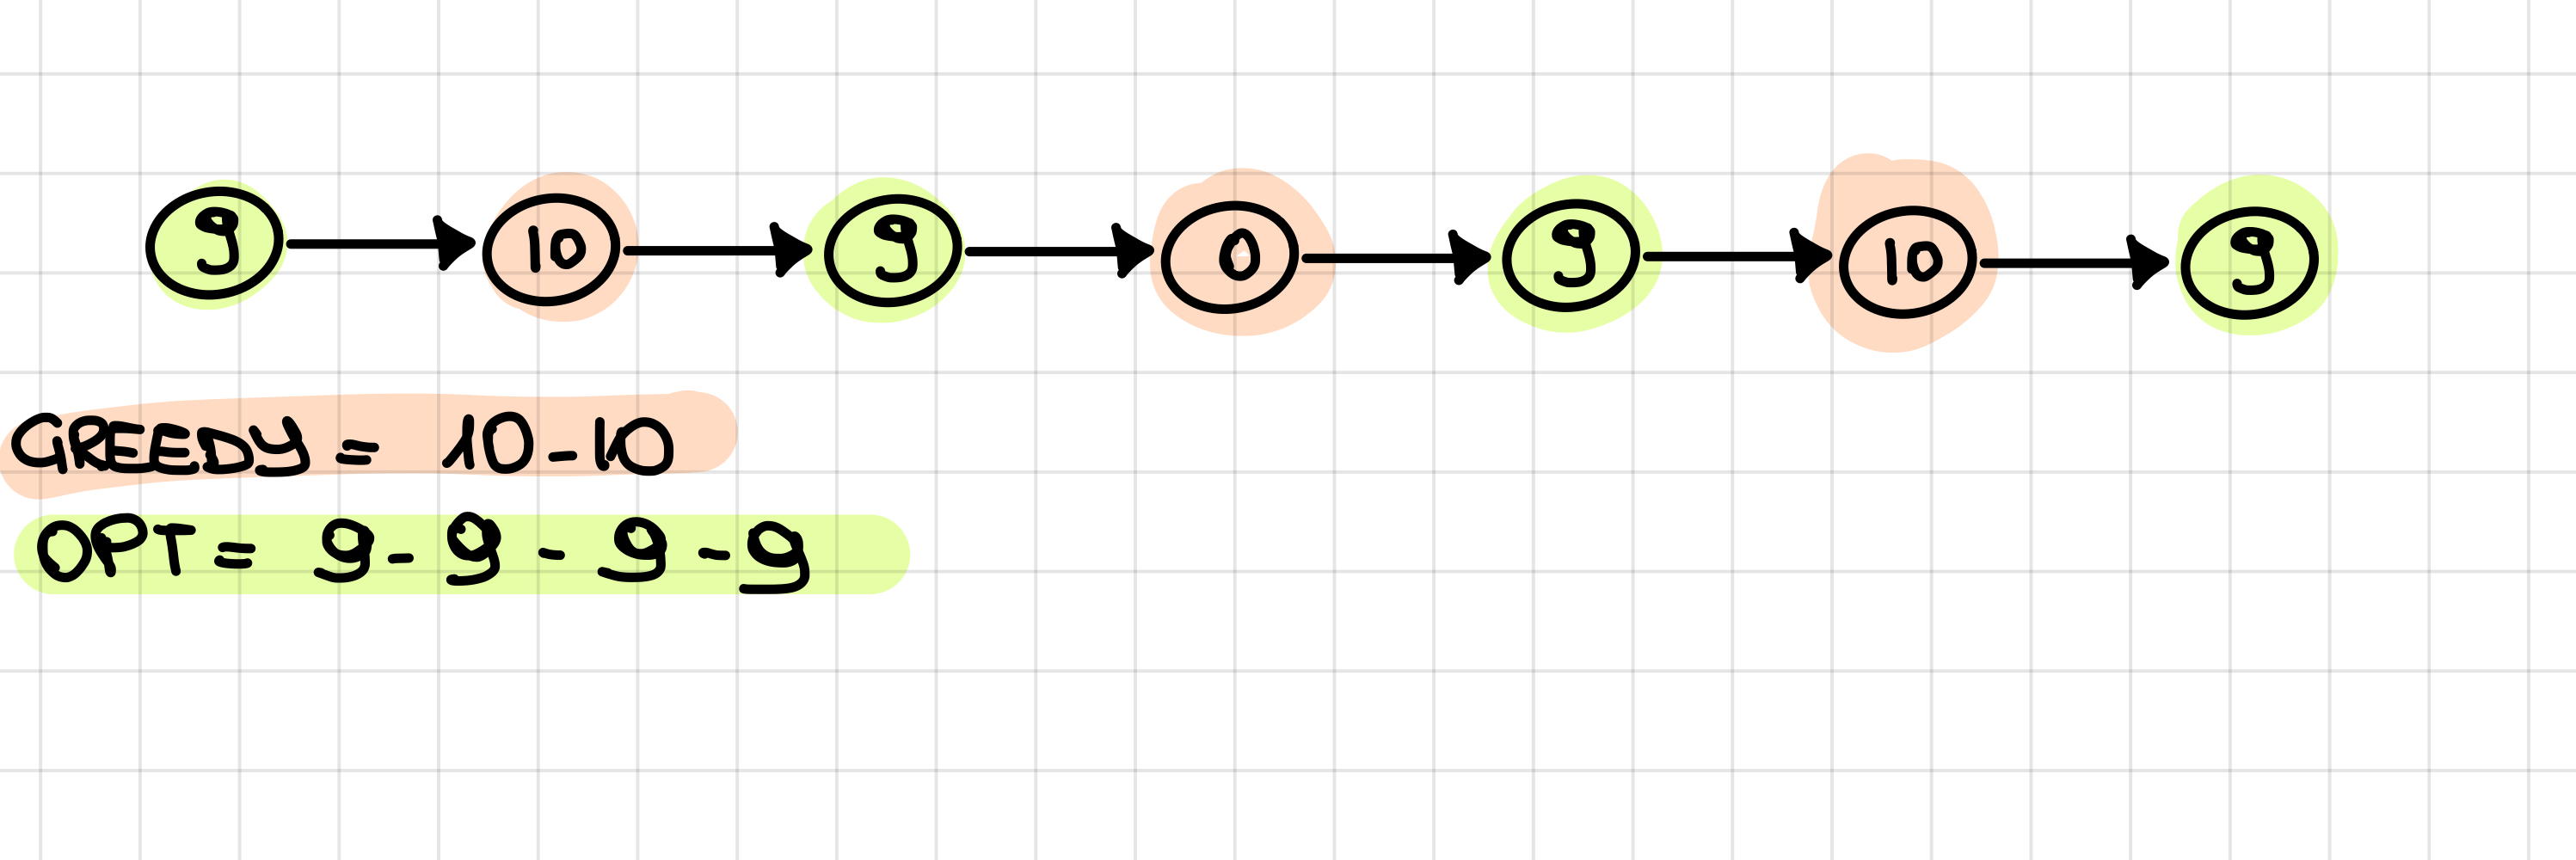
\includegraphics[width=0.7\textwidth]{imm/Immagine JPEG-4E60-AE75-26-0.jpeg}
\end{figure}

  \item[(b)] We can solve this problem using dynamic programming. We define $\text{OPT}(i)$ as the maximum total weight of an independent set that can be formed from the first $i$ nodes.
\[
\text{OPT}(i) = 
\begin{cases}
0 & \text{se } i = 0 \\
w_1 & \text{se } i = 1 \\
\max\left\{ \text{OPT}(i-1),\; \text{OPT}(i-2) + w_i \right\} & \text{se } i \geq 2
\end{cases}
\]
  \item [(c)] The pseudo-code of the algorithm is as follows:
\begin{lstlisting}[language=Python]
def max_independent_set(weights):
    n = len(weights)
    OPT[0] = 0
    OPT[1] = weights[1]
    for i =2 to n:
        if weights[i] + OPT[i - 2] > OPT[i - 1]:
            OPT[i] = weights[i] + OPT[i - 2]
        else:
            OPT[i] = OPT[i - 1]
    return OPT[n]
\end{lstlisting}
example of the algorithm in action:
\begin{figure}[H]
\centering
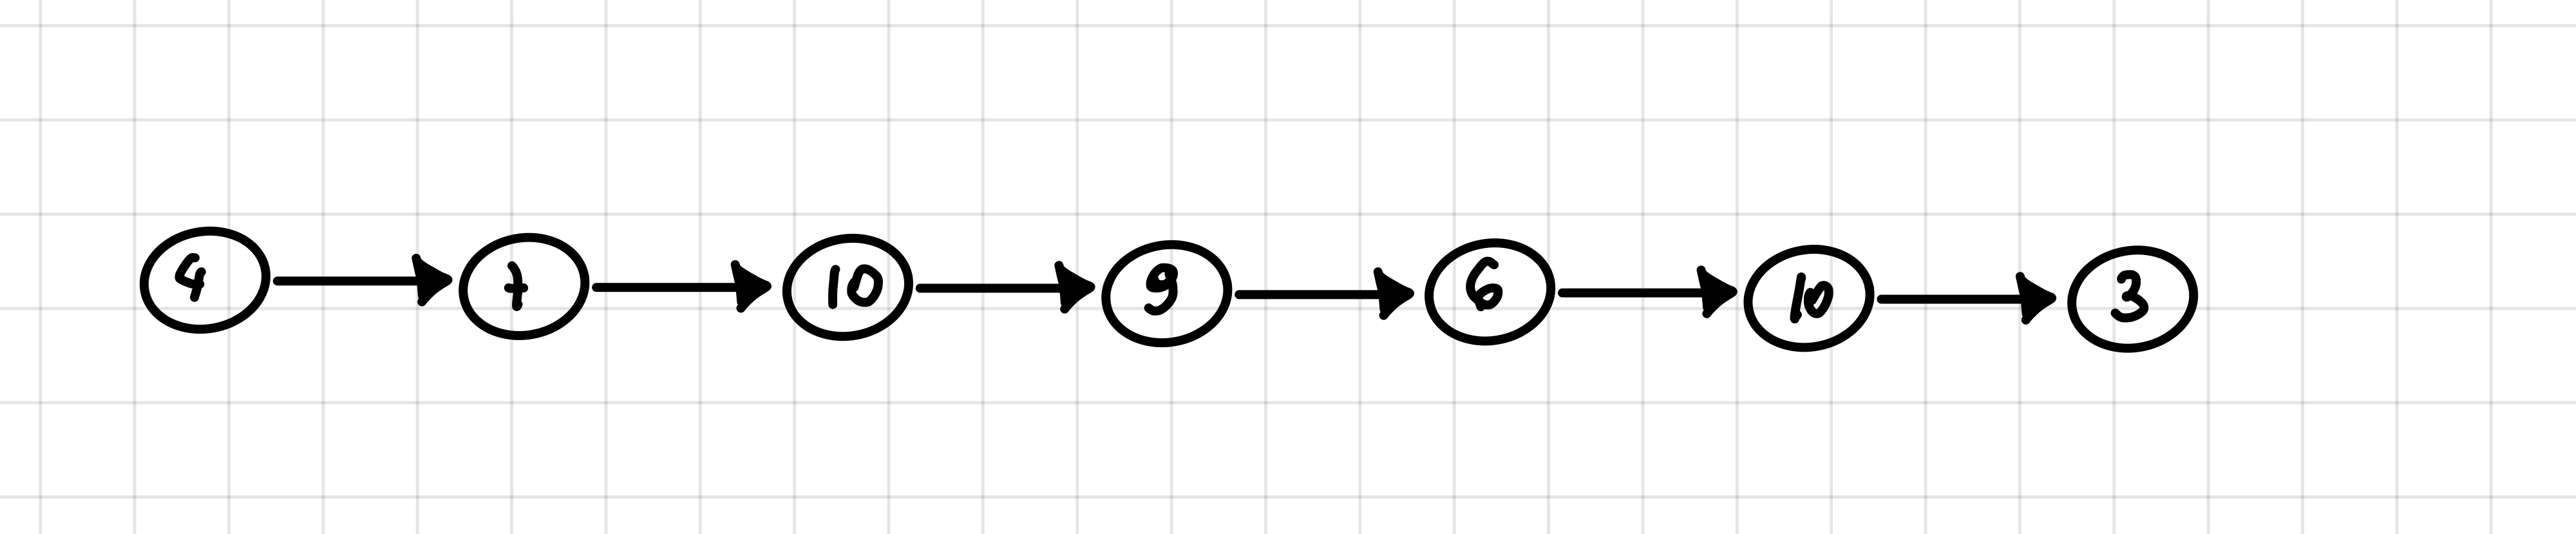
\includegraphics[width=0.7\textwidth]{imm/Immagine JPEG-4577-94E5-C9-0.jpeg}
\end{figure}
\begin{align*}
\text{OPT}(0) &= 0 \\
\text{OPT}(1) &= 4 \\
\text{OPT}(2) &= \max\{ \text{OPT}(1),\; \text{OPT}(0) + 7 \} = \max\{4, 7\} = 7 \\
\text{OPT}(3) &= \max\{ \text{OPT}(2),\; \text{OPT}(1) + 10 \} = \max\{7, 14\} = 14 \\
\text{OPT}(4) &= \max\{ \text{OPT}(3),\; \text{OPT}(2) + 9 \} = \max\{14, 16\} = 16 \\
\text{OPT}(5) &= \max\{ \text{OPT}(4),\; \text{OPT}(3) + 6 \} = \max\{16, 20\} = 20 \\
\text{OPT}(6) &= \max\{ \text{OPT}(5),\; \text{OPT}(4) + 10 \} = \max\{20, 26\} = 26 \\
\text{OPT}(7) &= \max\{ \text{OPT}(6),\; \text{OPT}(5) + 3 \} = \max\{26, 23\} = 26 \\
\end{align*}
algorithm to know which nodes are in the optimal solution:
\begin{lstlisting}[language=Python]
def find_solution(OPT, weights, i):
    i = len(weights)
    if i=0:
        return []
    if i=1:
        return [1]
    if weights[i] + OPT[i - 2] > OPT[i - 1]:
        return find_solution(OPT, weights, i - 2) + [i]
    else:
        return find_solution(OPT, weights, i - 1)
\end{lstlisting}
\end{enumerate}



\textbf{Problem 2 (Rod Cutting)}

We are given a rod of integer length $L$. We assume that a rod of integer
length $0 \leq l \leq L$ has a known value $v(l)$. The problem is to find
the best way of cutting the rod, such that the sum of the values of the
resulting rods is maximised.

\begin{enumerate}
  \item[(a)] Show a dynamic programming algorithm that solves the problem.
  \item[(b)] Prove the correctness of the recursive form used, and the optimality of the solution returned by the algorithm.
  \item[(c)] Provide the pseudo-code of an efficient implementation of the
            algorithm and discuss its time complexity.
\end{enumerate}
\textbf{Solution}

\begin{enumerate}
    \item[(a)] We can solve this problem using dynamic programming. 
    Let $v(i)$ be the value of a rod of length $i$, and $R(l)$ be the maximum value obtainable for a rod of length $l$.
    
    The optimal substructure of the problem allows us to define the following recurrence:
    \[
    R(l) = 
    \begin{cases}
    0 & \text{if } l = 0 \\
    \max_{1 \leq j \leq l} \left\{ v(j) + R(l-j) \right\} & \text{if } l > 0
    \end{cases}
    \]

    \item[(b)] \textbf{Proof of Correctness}: 
    An optimal cut for a rod of length $l$ consists of a first piece of length $j$ and an optimal arrangement of the remaining $l-j$ length. Since the value of the first piece $v(j)$ is fixed, to maximize the total value we must maximize the value of the remaining part, which is $R(l-j)$. By iterating over all possible first cuts $j \in \{1, \dots, l\}$, we are guaranteed to find the global maximum.
    % --- Il tuo TikZ (ottimizzato) ---
\begin{center}
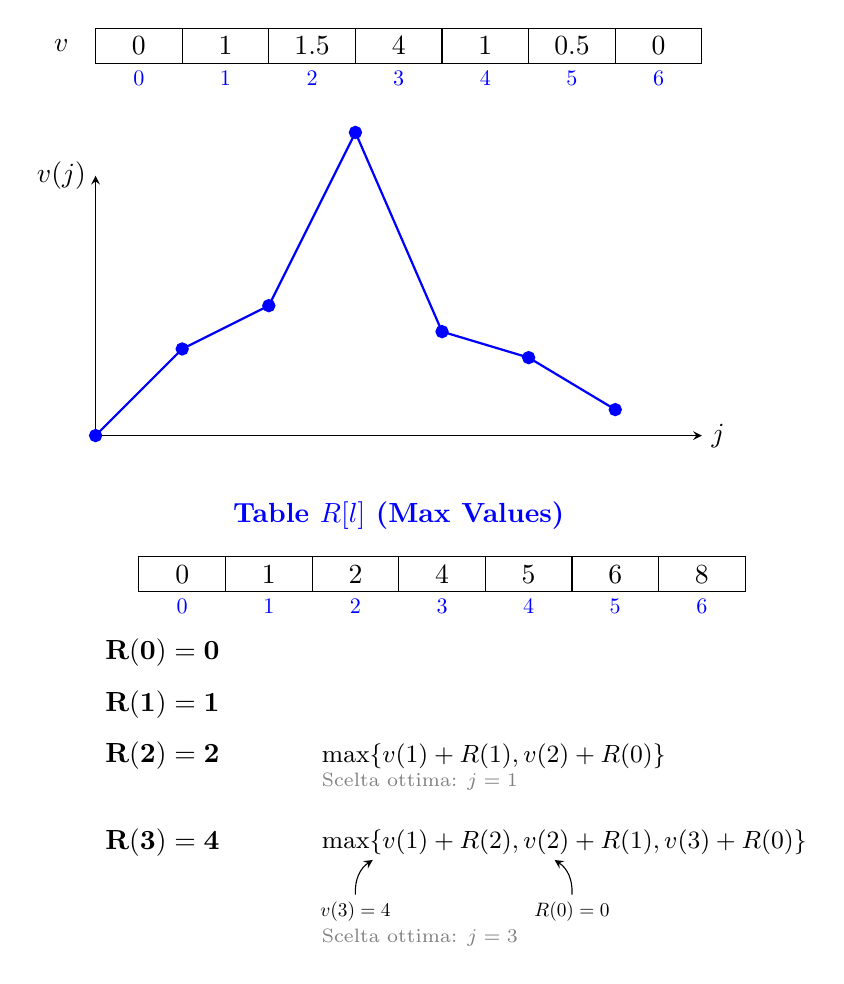
\begin{tikzpicture}[x=1.1cm, y=1.1cm, >=stealth]
    % Tabella v
    \node[left] at (-0.2, 4.5) {$v$};
    \foreach \x/\val [count=\i from 0] in {0/0, 1/1, 2/1.5, 3/4, 4/1, 5/0.5, 6/0} {
        \draw (\i, 4.3) rectangle (\i+1, 4.7);
        \node at (\i+0.5, 4.5) {\val};
        \node[blue, below, scale=0.8] at (\i+0.5, 4.3) {\i};
    }
    
    % Grafico
    \draw[->] (0,0) -- (0,3) node[left] {$v(j)$};
    \draw[->] (0,0) -- (7,0) node[right] {$j$};
    \draw[blue, thick, mark=*] plot coordinates {(0,0) (1,1) (2,1.5) (3,3.5) (4,1.2) (5,0.9) (6,0.3)};

    % Tabella Rod
    \node[blue, above] at (3.5, -1.2) {\textbf{Table $R[l]$ (Max Values)}}; 
    \foreach \x/\val [count=\i from 0] in {0/0, 1/1, 2/2, 3/4, 4/5, 5/6, 6/8} {
        \draw (\i+0.5, -1.8) rectangle (\i+1.5, -1.4);
        \node at (\i+1, -1.6) {\val};
        \node[blue, below, scale=0.8] at (\i+1, -1.8) {\i};
    }
    % Dettaglio Calcoli Incolonnati
\begin{scope}[shift={(0,-2.5)}]
    \node[anchor=west] at (0, 0) {$\mathbf{R(0)=0}$};
    \node[anchor=west] at (0, -0.6) {$\mathbf{R(1)=1}$};
    
    % R(2)
    \node[anchor=west] at (0, -1.2) {$\mathbf{R(2)=2}$};
    \node[anchor=west, font=\small] at (2.5, -1.2) {$\max \{ v(1)+R(1), v(2)+R(0) \}$};
    \node[anchor=west, font=\scriptsize, gray] at (2.5, -1.5) {Scelta ottima: $j=1$};

    % R(3)
    \node[anchor=west] at (0, -2.2) {$\mathbf{R(3)=4}$};
    \node[anchor=west, font=\small] at (2.5, -2.2) {$\max \{ v(1)+R(2), v(2)+R(1), v(3)+R(0) \}$};
    
    % Frecce logiche per R(3)
    \draw[->, bend left] (3, -2.8) to (3.2, -2.4);
    \node[below, scale=0.7] at (3, -2.8) {$v(3)=4$};
    
    \draw[->, bend right] (5.5, -2.8) to (5.3, -2.4);
    \node[below, scale=0.7] at (5.5, -2.8) {$R(0)=0$};
    
    \node[anchor=west, font=\scriptsize, gray] at (2.5, -3.3) {Scelta ottima: $j=3$};
\end{scope}
\end{tikzpicture}
\end{center}

  \item[(c)] \textbf{Implementation and Complexity}:

First, we consider the basic \textit{bottom-up} implementation that computes only the maximum revenue $R[L]$:

\begin{lstlisting}[language=Python, caption={Basic Bottom-Up Rod Cutting}]
def rod_cutting(v, L):
    R = [0] * (L + 1)
    for j in range(1, L + 1):
        q = float('-inf')
        for k in range(1, j + 1):
            q = max(q, v[k] + R[j - k])
        R[j] = q
    return R[L]
\end{lstlisting}

To reconstruct the actual cuts used to achieve this maximum, we extend the algorithm by using an auxiliary array $S$ to store the length of the first piece $i$ that achieved the maximum revenue for each subproblem $j$:

\begin{lstlisting}[language=Python, caption={Extended Bottom-Up Rod Cutting}]
def extended_bottom_up_rod_cutting(v, L):
    R = [0] * (L + 1)
    S = [0] * (L + 1)
    for j in range(1, L + 1):
        q = float('-inf')
        for i in range(1, j + 1):
            if q < v[i] + R[j - i]:
                q = v[i] + R[j - i]
                S[j] = i
        R[j] = q
    return R, S
\end{lstlisting}



\textbf{Complexity Analysis}:
\begin{itemize}
    \item \textbf{Time Complexity}: $O(L^2)$. The nested loops result in a summation $\sum_{j=1}^{L} j = \frac{L(L+1)}{2}$, which is quadratic.
    \item \textbf{Space Complexity}: $O(L)$ to store the memoization table $R$ and the optimal cuts $S$.
\end{itemize}

\textbf{Solution Reconstruction}:
To print the lengths of the pieces in an optimal solution for length $L$:
\begin{lstlisting}[language=Python]
def print_optimal_cuts(S, L):
    while L > 0:
        print(S[L])
        L = L - S[L]
\end{lstlisting}
\end{enumerate}
\chapter{Network Flow}

\section{Max-Flow and Min-Cut Problems}

Max-flow and min-cut are two fundamental problems in network flow theory,
defined on a directed graph $G = (V, E)$ with a source node $s$, a sink
node $t$, and a capacity function $c : E \to \mathbb{R}^+$ that assigns a
non-negative capacity to each edge.

\begin{figure}[H]
    \centering
    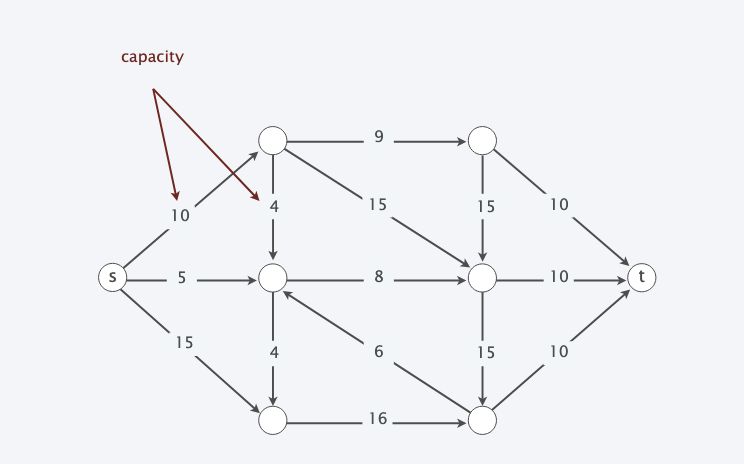
\includegraphics[width=0.5\textwidth]{imm/Screenshot 2026-03-30 alle 08.33.35.png}
    \caption{Example of a flow network with source $s$, sink $t$, and edge capacities.}
\end{figure}

\begin{definition}
    An \emph{st-cut} (cut) is a partition $(A, B)$ of the vertices such that
    $s \in A$ and $t \in B$.
\end{definition}

\begin{definition}
    The \emph{capacity} of an st-cut $(A, B)$ is the sum of the capacities
    of edges going \emph{from} $A$ \emph{to} $B$:
    \[
        \mathrm{cap}(A, B) = \sum_{\substack{e \,=\, (u,v) \\ u \in A,\; v \in B}} c(e).
    \]
    Edges from $B$ to $A$ are \textbf{not} counted.
\end{definition}

\textbf{Min-cut problem.} Find an st-cut of minimum capacity.

\begin{figure}[H]
    \centering
    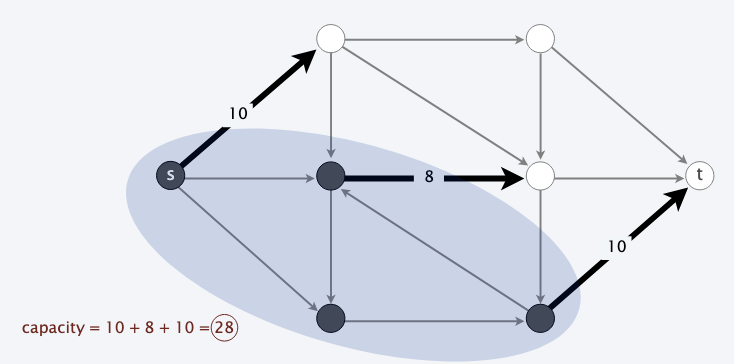
\includegraphics[width=0.5\textwidth]{imm/Screenshot 2026-03-30 alle 08.40.26.png}
    \caption{capacity of 28.}
\end{figure}

\begin{definition}
    An \emph{st-flow} is a function $f : E \to \mathbb{R}^+$ satisfying:
    \begin{itemize}
        \item \textbf{Capacity constraint}: For every edge $e \in E$,
              $0 \leq f(e) \leq c(e)$.
              un arco non può trasportare più del suo limite di capacità.
        \item \textbf{Flow conservation}: For every vertex $v \in V \setminus
              \{s, t\}$, the total flow into $v$ equals the total flow out of
              $v$:
              \[
                  \sum_{\substack{e \,=\, (u,v) \\ (u,v) \in E}} f(e)
                  \;=\;
                  \sum_{\substack{e \,=\, (v,w) \\ (v,w) \in E}} f(e).
              \]
                un nodo che non è né la sorgente né il pozzo non può accumulare
                flusso, quindi tutto quello che entra deve uscire.
    \end{itemize}
\end{definition}

\begin{definition}
    The \emph{value} of a flow $f$ is
    \[
        \mathrm{val}(f) = \sum_{e \text{ out of } s} f(e),
    \]
    i.e., the total flow leaving the source $s$.
\end{definition}

\textbf{Max-flow problem.} Find an st-flow of maximum value.

\begin{figure}[H]
    \centering
    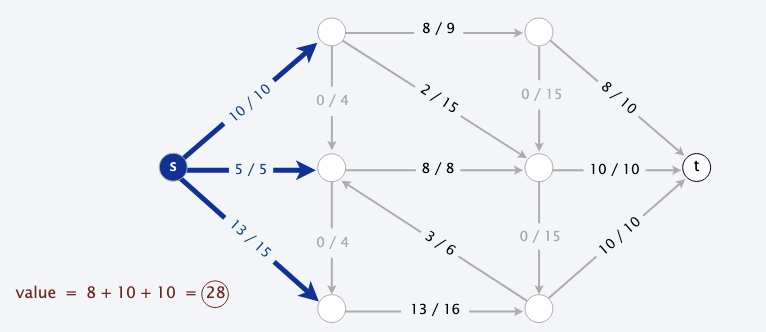
\includegraphics[width=0.5\textwidth]{imm/Screenshot 2026-03-30 alle 08.47.19.png}
    \caption{Example of a maximum flow with value 28.}
\end{figure}

% -------------------------------------------------------------------
\section{Ford-Fulkerson Algorithm}

\subsection{Greedy Approach and Its Limits}

A natural greedy strategy is:
\begin{itemize}
    \item Start with $f(e) = 0$ for all edges $e \in E$.
    \item Find an st-path $P$ where every edge $e$ satisfies $f(e) < c(e)$
          (i.e., has remaining capacity).
    \item Push as much flow as possible along $P$ (limited by the minimum
          remaining capacity on the path).
    \item Repeat until no such path exists.
\end{itemize}

\textbf{Problem with the greedy approach.} The order in which augmenting
paths are chosen can cause the algorithm to terminate with a sub-optimal
flow. For instance, on certain networks the greedy approach reaches a flow
of value 16, even though the true maximum is 19. This happens because
saturating some edges blocks all remaining paths from $s$ to $t$, even
when additional flow could theoretically be routed differently.
\begin{figure}[H]
    \centering
    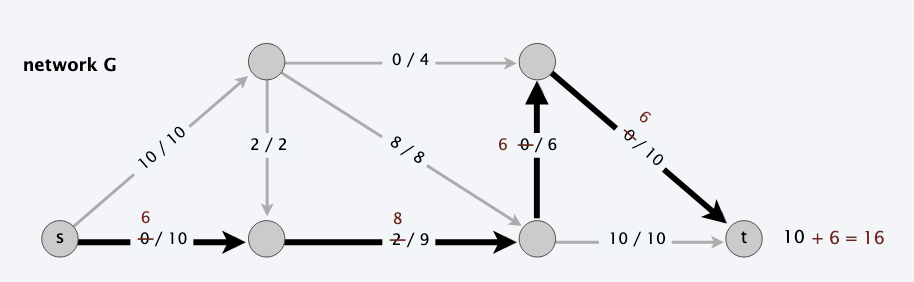
\includegraphics[width=0.5\textwidth]{imm/Screenshot 2026-03-30 alle 09.21.45.png}
    \caption{Along the augmenting path s→2→4→t, the bottleneck is 8 (limited by edge 2→4, capacity 8), bringing the total flow to 8. Edge s→2 still has 10 $-$ 8 = 2 units of residual capacity, which are routed along path s→2→3→4→t through edge 2→3 (capacity 2), saturating s→2 and raising the total flow to 10. Finally, the augmenting path s→3→4→5→t has bottleneck 6, yielding a total flow of 10 + 6 = 16.}
\end{figure}

\begin{figure}[H]
    \centering
    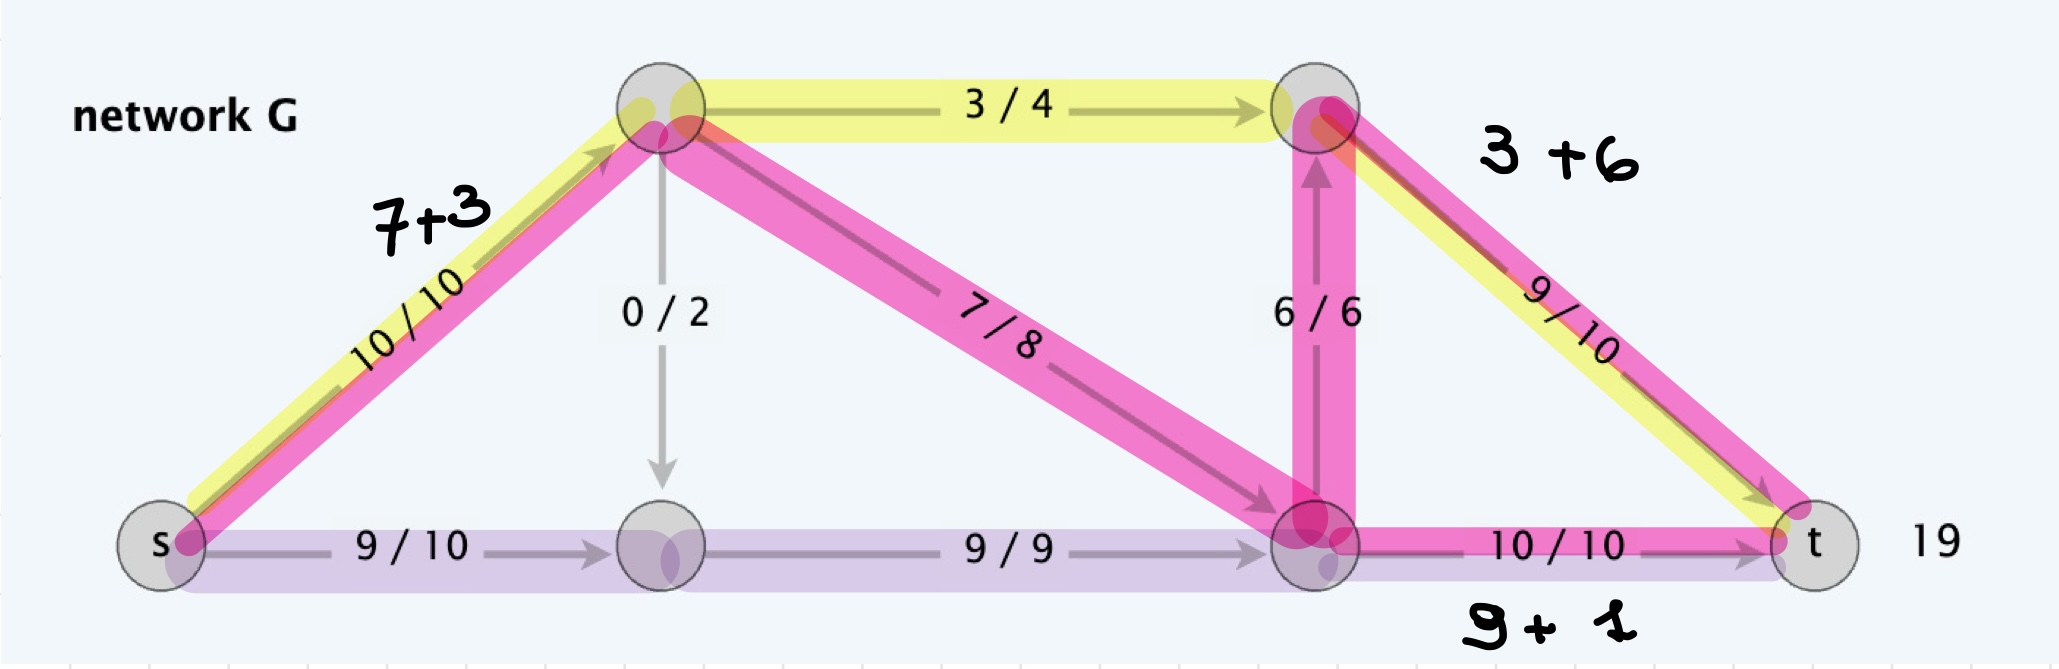
\includegraphics[width=0.5\textwidth]{imm/Immagine JPEG-46B2-83B7-C2-0.jpeg}
    \caption{}
\end{figure}

The solution is to use a \emph{residual graph} that allows the algorithm
to \emph{undo} previously sent flow, which is the core idea behind
Ford-Fulkerson.

\subsection{Residual Graph}

\begin{definition}
    Given a flow network $G = (V, E)$ and a flow $f$, the
    \emph{residual graph} $G_f = (V, E_f)$ is constructed as follows.
    For each original edge $e = (u, v) \in E$ with capacity $c(e)$ and
    flow $f(e)$, we create:
    \begin{itemize}
        \item A \emph{forward residual edge} $e = (u, v)$ with residual
              capacity $c_f(e) = c(e) - f(e)$, representing the remaining
              capacity (included only if $c_f(e) > 0$, i.e., $f(e) < c(e)$).
              \begin{figure}[H]
                                \centering
                                \begin{minipage}{0.44\textwidth}
                                    \centering
                                    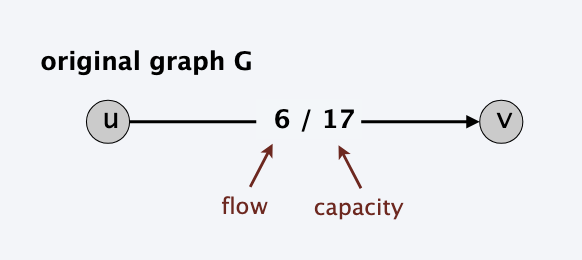
\includegraphics[width=\textwidth]{imm/Screenshot 2026-03-30 alle 09.32.43.png}
                                \end{minipage}\hfill
                                \begin{minipage}{0.54\textwidth}
                                    \centering
                                    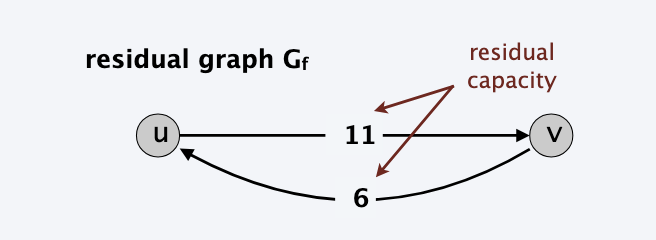
\includegraphics[width=\textwidth]{imm/Screenshot 2026-03-30 alle 09.32.52.png}
                                \end{minipage}
                                \caption{The forward residual edge from $u$ to $v$ has capacity $c(e) - f(e)$.}
                          \end{figure}
              \item A \emph{backward residual edge} $e^R = (v, u)$ with residual
              capacity $c_f(e^R) = f(e)$, representing the flow that can be
              \emph{cancelled} (included only if $f(e) > 0$).
    \end{itemize}
    Formally:
    \[
        E_f = \bigl\{e \in E : f(e) < c(e)\bigr\}
              \;\cup\;
              \bigl\{e^R : e \in E,\; f(e) > 0\bigr\},
    \]
    \[
        c_f(e) =
        \begin{cases}
            c(e) - f(e) & \text{if } e \in E, \\
            f(e)        & \text{if } e^R \in E.
        \end{cases}
    \]
\end{definition}

\textbf{Key property.} A flow $f'$ in $G_f$ corresponds to a valid flow
$f + f'$ in the original graph $G$.

\subsection{Augmenting Path}

\begin{definition}
    An \emph{augmenting path} is a simple st-path $P$ in the residual graph
    $G_f$ such that every edge on $P$ has strictly positive residual capacity.
\end{definition}

\begin{definition}
    The \emph{bottleneck capacity} of an augmenting path $P$ in $G_f$ is
    \[
        \mathrm{bottleneck}(G_f, P)
        = \min_{e \in P} c_f(e),
    \]
    i.e., the minimum residual capacity among all edges on $P$.
    It is the maximum amount of additional flow that can be pushed
    along $P$ without violating any capacity constraint.
\end{definition}

\textbf{Key property.} Let $f$ be a flow in $G$ and $P$ be an augmenting
path in $G_f$. Let $b = \mathrm{bottleneck}(G_f, P)$. After augmenting
along $P$:
\[
    \mathrm{val}(f') = \mathrm{val}(f) + b.
\]

\begin{figure}[H]
    \centering
    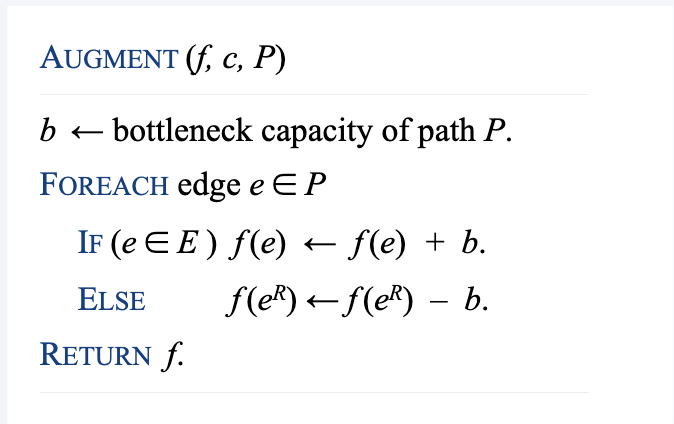
\includegraphics[width=0.5\textwidth]{imm/Screenshot 2026-03-30 alle 09.33.50.png}
   
\end{figure}


\subsection{Ford-Fulkerson Algorithm}

\begin{figure}[H]
    \centering
    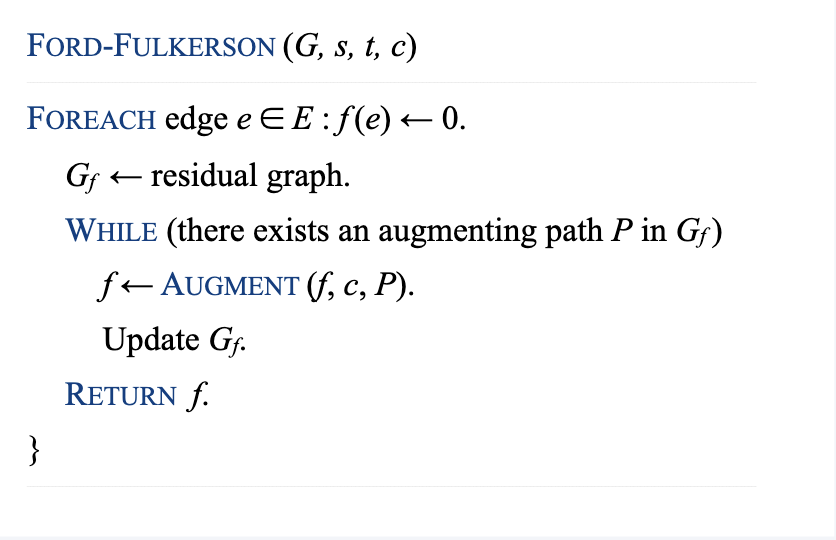
\includegraphics[width=0.5\textwidth]{imm/Screenshot 2026-03-30 alle 09.35.20.png}
\end{figure}

\subsection*{example}
\begin{figure}[H]
    \centering
    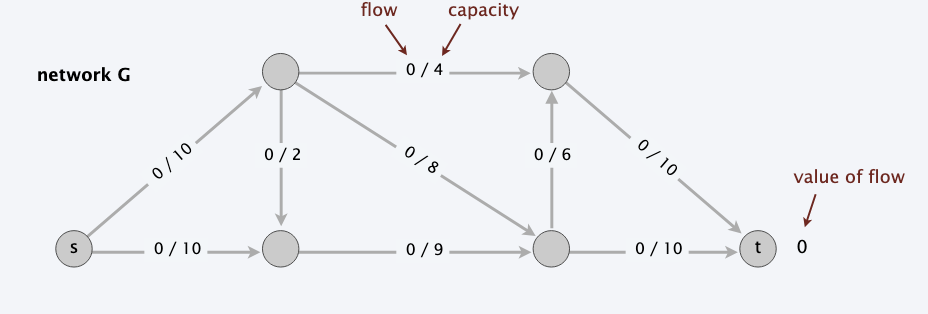
\includegraphics[width=0.5\textwidth]{imm/Screenshot 2026-03-30 alle 08.57.26.png}
\end{figure}
\paragraph{Step 1.}
Find an augmenting path $P_1$ in the residual graph $G_f$.
The bottleneck capacity is 8. Augment along $P_1$:
\[
    \mathrm{val}(f) = 0 + 8 = 8.
\]

\paragraph{Step 2.}
Find a new augmenting path $P_2$ in the updated residual graph.
The bottleneck capacity is 2. Augment along $P_2$:
\[
    \mathrm{val}(f) = 8 + 2 = 10.
\]
\begin{figure}[H]
    \centering
    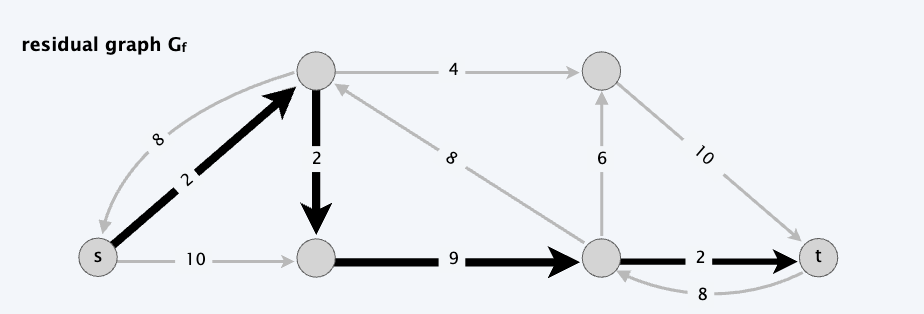
\includegraphics[width=0.5\textwidth]{imm/Screenshot 2026-04-14 alle 15.30.02.png}
\end{figure}
\paragraph{Step 3.}
Find augmenting path $P_3$ with bottleneck capacity 6:
\[
    \mathrm{val}(f) = 10 + 6 = 16.
\]

At this point, a purely greedy algorithm (without the residual graph)
would get stuck: no forward-edge-only path from $s$ to $t$ remains.
However, the residual graph $G_f$ still contains augmenting paths that
use \textbf{backward edges} to ``reroute'' flow already sent.

\paragraph{Step 4 — use of a backward edge.}
In $G_f$, there exists a path $P_4$ that traverses a backward
(reverse) residual edge. Sending flow along a backward edge
\emph{cancels} part of a previously assigned flow, effectively
rerouting it. The bottleneck capacity is 2:
\[
    \mathrm{val}(f) = 16 + 2 = 18.
\]
\paragraph{Step 5.}
One further augmenting path $P_5$ with bottleneck capacity 1:
\[
    \mathrm{val}(f) = 18 + 1 = 19.
\]
\begin{figure}[H]
    \centering
    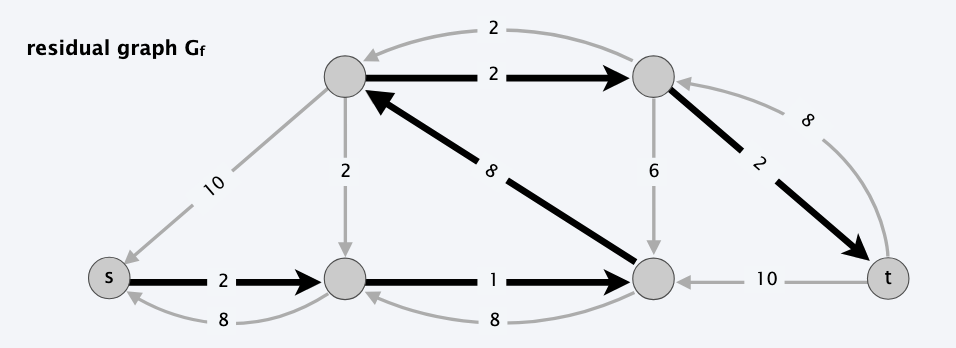
\includegraphics[width=0.5\textwidth]{imm/Screenshot 2026-03-30 alle 09.37.37.png}
\end{figure}
After step 5 there is no augmenting path in $G_f$, so the algorithm
terminates.

% -------------------------------------------------------------------
\section{Max-Flow Min-Cut Theorem}

The Max-Flow Min-Cut Theorem establishes a fundamental duality between
flows and cuts: the maximum value of any st-flow equals the minimum
capacity of any st-cut. We build towards this result in three steps.

% -------------------------------------------------------------------
\subsection{Flow Value Lemma}

\begin{lemma}[Flow Value Lemma]
    Let $f$ be any st-flow and let $(A, B)$ be any st-cut. Then the
    \emph{net flow} across $(A, B)$ equals the value of $f$:
    \[
        \mathrm{val}(f)
        = \sum_{\substack{e \,=\,(u,v) \\ u \in A,\; v \in B}} f(e)
        \;-\;
        \sum_{\substack{e \,=\,(u,v) \\ u \in B,\; v \in A}} f(e).
    \]
\end{lemma}

\begin{proof}
By definition, $\mathrm{val}(f) = \sum_{e \text{ out of } s} f(e)$.
We extend the sum over all nodes in $A$:
\[
    \mathrm{val}(f)
    = \sum_{v \in A}
      \left(
        \sum_{e \text{ out of } v} f(e)
        - \sum_{e \text{ into } v} f(e)
      \right).
\]
By \textbf{flow conservation}, every term with $v \neq s$ vanishes.
Rearranging the remaining terms by whether the edge crosses the cut
$(A \to B)$ or goes backwards $(B \to A)$ yields the result.
\end{proof}

    Edges entirely within $A$ or within $B$ cancel out in the sum,
    so only edges \emph{crossing} the cut contribute to $\mathrm{val}(f)$.


% -------------------------------------------------------------------
\subsection{Weak Duality}

\begin{corollary}[Weak Duality]
    For any st-flow $f$ and any st-cut $(A, B)$:
    \[
        \mathrm{val}(f) \;\leq\; \mathrm{cap}(A, B).
    \]
\end{corollary}

\begin{proof}
Using the Flow Value Lemma and the capacity constraint $f(e) \leq c(e)$:
\[
    \mathrm{val}(f)
    = \sum_{\substack{e \text{ out of } A}} f(e)
    - \sum_{\substack{e \text{ into } A}} f(e)
    \;\leq\;
    \sum_{\substack{e \text{ out of } A}} f(e)
    \;\leq\;
    \sum_{\substack{e \text{ out of } A}} c(e)
    = \mathrm{cap}(A,B).
\]
\end{proof}

Weak duality immediately implies that any flow value is an
\emph{upper bound} on every cut capacity, and vice versa.
In particular, if we ever find a flow $f$ and a cut $(A,B)$
such that $\mathrm{val}(f) = \mathrm{cap}(A,B)$, both must be
simultaneously optimal.

% -------------------------------------------------------------------
\section{Max-Flow Min-Cut Theorem}

\begin{theorem}[Max-Flow Min-Cut Theorem]
    In any flow network, the value of a maximum st-flow equals the
    capacity of a minimum st-cut:
    \[
        \max_{f} \,\mathrm{val}(f)
        \;=\;
        \min_{(A,B)} \mathrm{cap}(A,B).
    \]
\end{theorem}

\begin{proof}
We prove the equivalence of the following three conditions for any
flow $f$:
\begin{enumerate}[label=(\roman*)]
    \item There exists an st-cut $(A,B)$ such that
          $\mathrm{cap}(A,B) = \mathrm{val}(f)$.
    \item $f$ is a maximum flow.
    \item There is no augmenting path in the residual graph $G_f$.
\end{enumerate}

\medskip
\noindent\textbf{(i) $\Rightarrow$ (ii).}
Suppose $(A,B)$ is a cut with $\mathrm{cap}(A,B) = \mathrm{val}(f)$.
For any other flow $f'$, weak duality gives
$\mathrm{val}(f') \leq \mathrm{cap}(A,B) = \mathrm{val}(f)$,
so $f$ is a maximum flow.

\medskip
\noindent\textbf{(ii) $\Rightarrow$ (iii).}
We prove the contrapositive.
If there exists an augmenting path $P$ in $G_f$, then we can
strictly increase $\mathrm{val}(f)$ by pushing
$\mathrm{bottleneck}(G_f, P) > 0$ additional units of flow along $P$.
Hence $f$ is not a maximum flow.

\medskip
\noindent\textbf{(iii) $\Rightarrow$ (i).}
Suppose no augmenting path exists in $G_f$. Define:
\[
    A = \{ v \in V : v \text{ is reachable from } s \text{ in } G_f \}.
\]
By definition, $s \in A$. Since there is no augmenting path, $t \notin A$,
so $(A, B = V \setminus A)$ is a valid st-cut.

Now consider any edge $e = (u,v)$ with $u \in A$, $v \in B$:
\begin{itemize}
    \item The forward residual edge $(u,v)$ cannot be in $G_f$
          (otherwise $v$ would be reachable), so $f(e) = c(e)$.
    \item Any edge $e' = (v,u)$ with $v \in B$, $u \in A$: the backward
          residual edge $(u,v)$ cannot be in $G_f$, so $f(e') = 0$.
\end{itemize}
Therefore, applying the Flow Value Lemma:
\[
    \mathrm{val}(f)
    = \sum_{\substack{e \text{ out of } A}} f(e)
    - \sum_{\substack{e \text{ into } A}} f(e)
    = \sum_{\substack{e \text{ out of } A}} c(e) - 0
    = \mathrm{cap}(A, B).
\]
\end{proof}

% -------------------------------------------------------------------
\subsection{Augmenting Path Theorem}

A direct consequence of the proof above is the following algorithmic
certificate:

\begin{corollary}[Augmenting Path Theorem]
    A flow $f$ is a maximum flow if and only if there is no augmenting
    path in the residual graph $G_f$.
\end{corollary}

This corollary is the theoretical foundation of the Ford-Fulkerson
algorithm: the algorithm terminates precisely when $f$ is optimal,
and at that point the set of nodes reachable from $s$ in $G_f$
defines the corresponding minimum cut.

\subsection*{Running Time}

\paragraph{Assumption}
All edge capacities are integers between $1$ and $C$.
    All edge capacities are integers between $1$ and $C$.

\begin{lemma}[Integrality Invariant]
    Throughout the Ford-Fulkerson algorithm, all flow values $f(e)$ and
    all residual capacities $c_f(e)$ remain integers.
\end{lemma}

\begin{proof}
    Initially all flows are 0. Each augmentation increases the flow
    along a path by $\mathrm{bottleneck}(G_f, P)$, which is the minimum
    of a finite set of integer residual capacities, hence an integer.
    By induction, all values remain integers throughout.
\end{proof}

\begin{theorem}
    The Ford-Fulkerson algorithm terminates in at most
    $\mathrm{val}(f^*) \leq nC$ iterations.
\end{theorem}

\begin{proof}
    By the integrality invariant, every augmentation increases
    $\mathrm{val}(f)$ by at least 1. Since $\mathrm{val}(f^*)$ is the
    maximum possible flow value and $\mathrm{val}(f^*) \leq nC$
    (at most $n$ edges out of $s$, each with capacity at most $C$),
    the algorithm terminates after at most $nC$ iterations.
\end{proof}

\begin{corollary}
    The running time of Ford-Fulkerson is $O(m \cdot n \cdot C)$, since
    each iteration requires $O(m)$ time to find an augmenting path via
    DFS or BFS.
\end{corollary}

\begin{corollary}
    If $C = 1$, the running time of Ford-Fulkerson reduces to $O(mn)$.
\end{corollary}

\begin{theorem}[Integrality Theorem]
    If all edge capacities are integers, then there exists a maximum
    flow $f^*$ in which every flow value $f^*(e)$ is an integer.
\end{theorem}

\begin{proof}
    Since all capacities are integers, the integrality invariant
    guarantees that the flow $f$ maintained by the algorithm is always
    integer-valued. Because the algorithm terminates (by the previous
    theorem), the flow upon termination is both a maximum flow and
    integer-valued.
\end{proof}

    Ford-Fulkerson is \textbf{not} a polynomial-time algorithm in general:
    its complexity $O(mnC)$ depends on the \emph{value} of the capacities,
    not just on the \emph{size} of the input. In the worst case, if
    $C$ is exponentially large, the algorithm takes exponentially many
    iterations. For polynomial guarantees, variants such as
    \textbf{Edmonds-Karp} (shortest augmenting path, $O(m^2 n)$) or
    \textbf{capacity scaling} ($O(m^2 \log C)$) must be used.
% -------------------------------------------------------------------   
\section{Capacity-Scaling Algorithm}

The basic Ford-Fulkerson algorithm can be very slow if it picks augmenting
paths with small bottleneck capacity. The \textbf{capacity-scaling algorithm}
fixes this by always working with large-capacity paths first.
\begin{figure}[H]
    \centering
    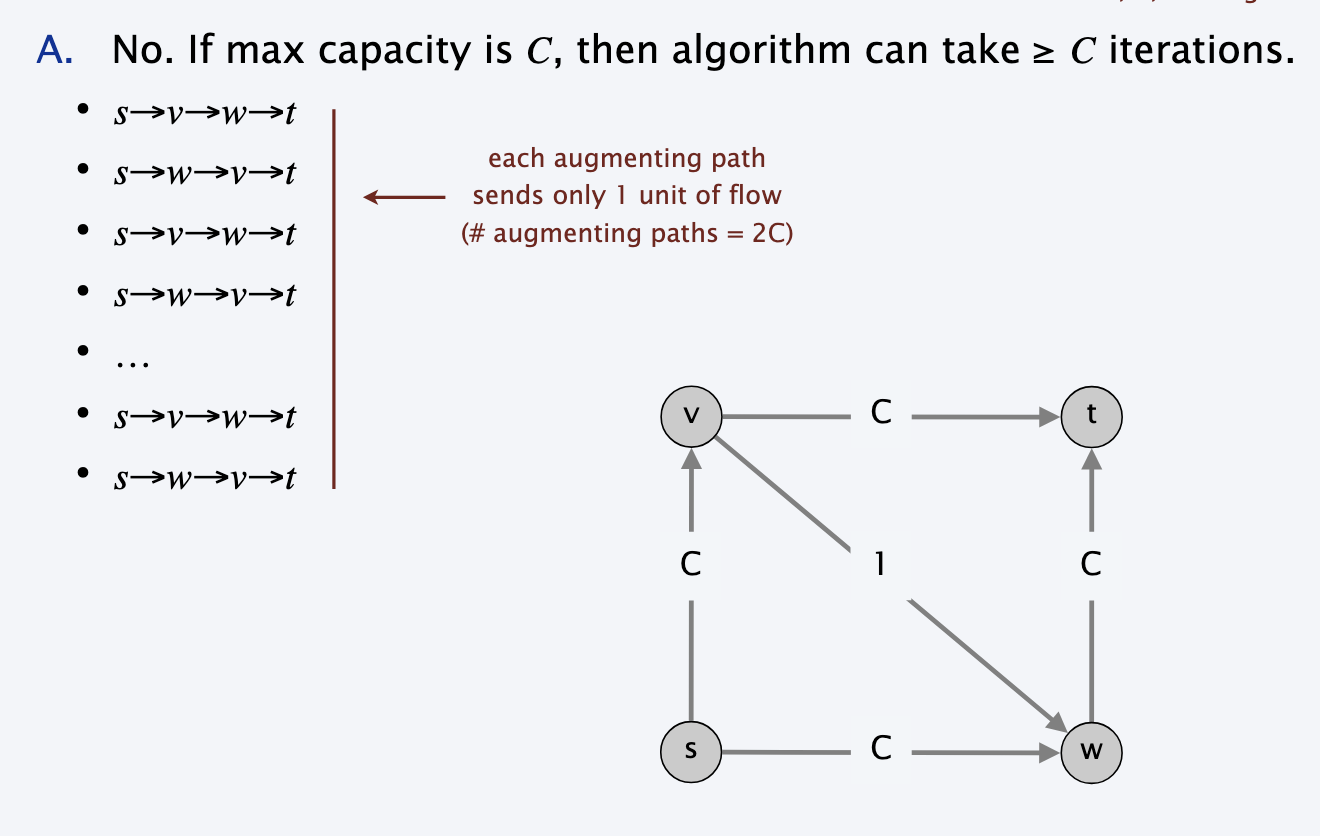
\includegraphics[width=0.5\textwidth]{imm/Screenshot 2026-04-16 alle 16.50.23.png}
\end{figure}
\subsubsection*{Key Idea}

Instead of using the full residual graph, we work on a restricted subgraph
$G_f(\Delta)$ that contains only edges with residual capacity $\geq \Delta$.
We start with $\Delta$ equal to the largest power of 2 that is $\leq C$
(the maximum capacity), and we halve $\Delta$ at each phase.

\begin{figure}[H]
    \centering
    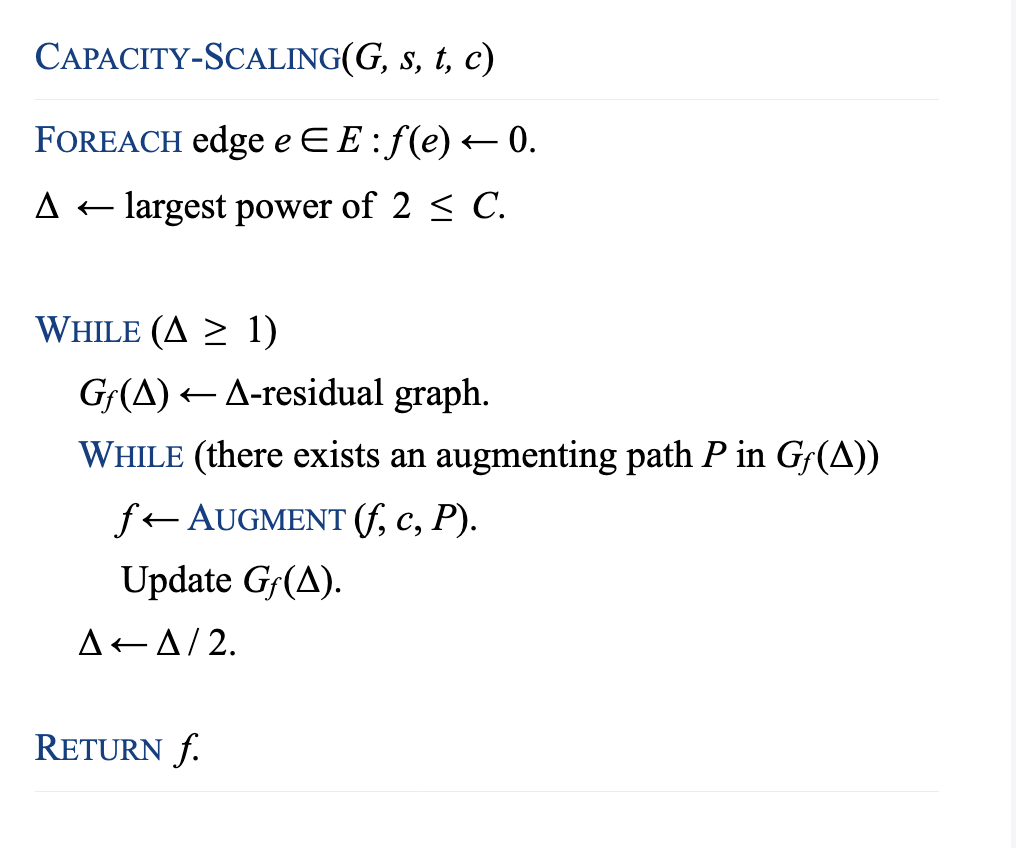
\includegraphics[width=0.8\textwidth]{imm/Screenshot 2026-04-16 alle 16.54.45.png}
\end{figure}

\subsubsection*{Correctness}

When $\Delta = 1$, the $\Delta$-residual graph equals the full residual graph.
So when the algorithm terminates, there are no augmenting paths in $G_f$,
which means $f$ is a max-flow by the Max-Flow Min-Cut theorem.

\subsubsection*{Running Time Analysis}

\begin{itemize}
    \item \textbf{Lemma 1.} The outer while loop runs at most $1 + \lfloor
    \log_2 C \rfloor$ times, since $\Delta$ starts at most $C$ and halves
    each time.
    \item \textbf{Lemma 2.} At the end of a $\Delta$-scaling phase, the
    value of the max-flow satisfies $\text{val}(f^*) \leq \text{val}(f) +
    2m\Delta$.
    \item \textbf{Lemma 3.} There are at most $2m$ augmentations per scaling
    phase. Each augmentation in a $\Delta$-phase increases the flow by at
    least $\Delta$, and by Lemma 2, at most $2m\Delta$ units remain to be
    added.
\end{itemize}

\begin{theorem}
The capacity-scaling algorithm finds a max-flow using $O(m \log C)$
augmentations and runs in $O(m^2 \log C)$ time.
\end{theorem}

\subsubsection*{Proof of Lemma 2}

At the end of a $\Delta$-scaling phase, let $A$ be the set of nodes
reachable from $s$ in $G_f(\Delta)$. Then $(A, B)$ is a cut, and every
edge from $A$ to $B$ has residual capacity $< \Delta$, so:
\[
\text{val}(f^*) \leq \text{val}(f) + \sum_{e \text{ out of } A} \Delta
\leq \text{val}(f) + m\Delta \leq \text{val}(f) + 2m\Delta.
\]

%------------------------------------------------------------
\section{Shortest Augmenting Paths}

Another way to improve Ford-Fulkerson is to always pick the augmenting path
with the \textbf{fewest edges}, found using BFS.

\begin{figure}[H]
    \centering
    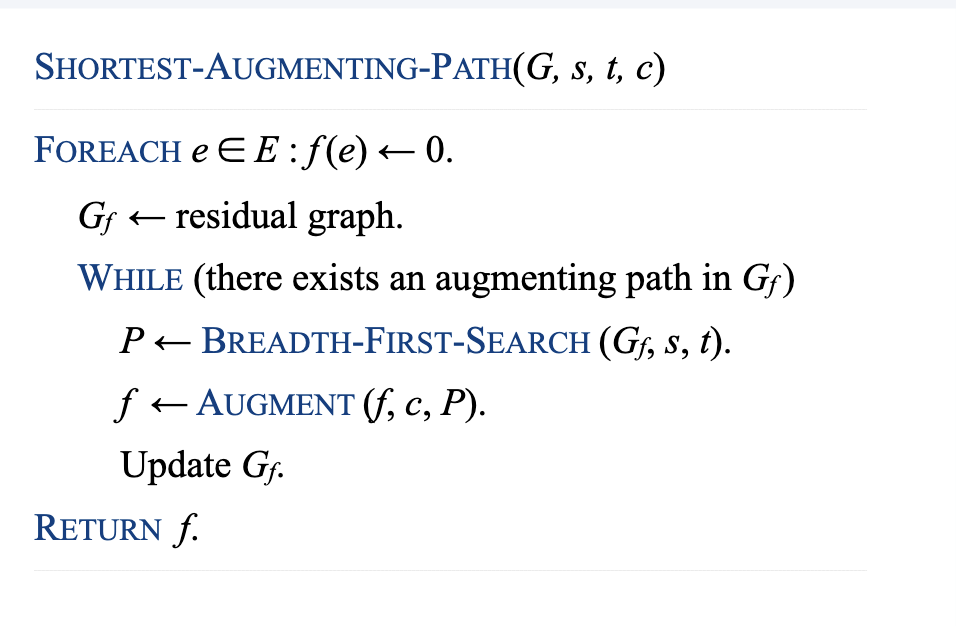
\includegraphics[width=0.7\textwidth]{imm/Screenshot 2026-04-16 alle 16.59.49.png}
\end{figure}

\subsection{Level Graph}

The \textbf{level graph} $L_G$ of a graph $G$ assigns to each node $v$ a
level $\ell(v)$ equal to the number of edges in the shortest path from $s$
to $v$. It contains only edges $(v, w)$ where $\ell(w) = \ell(v) + 1$.

A path is a shortest $s$-$v$ path in $G$ if and only if it is a path in
$L_G$. The level graph can be computed in $O(m + n)$ time by running BFS
and deleting all backward and side edges.

\begin{figure}[H]
    \centering
    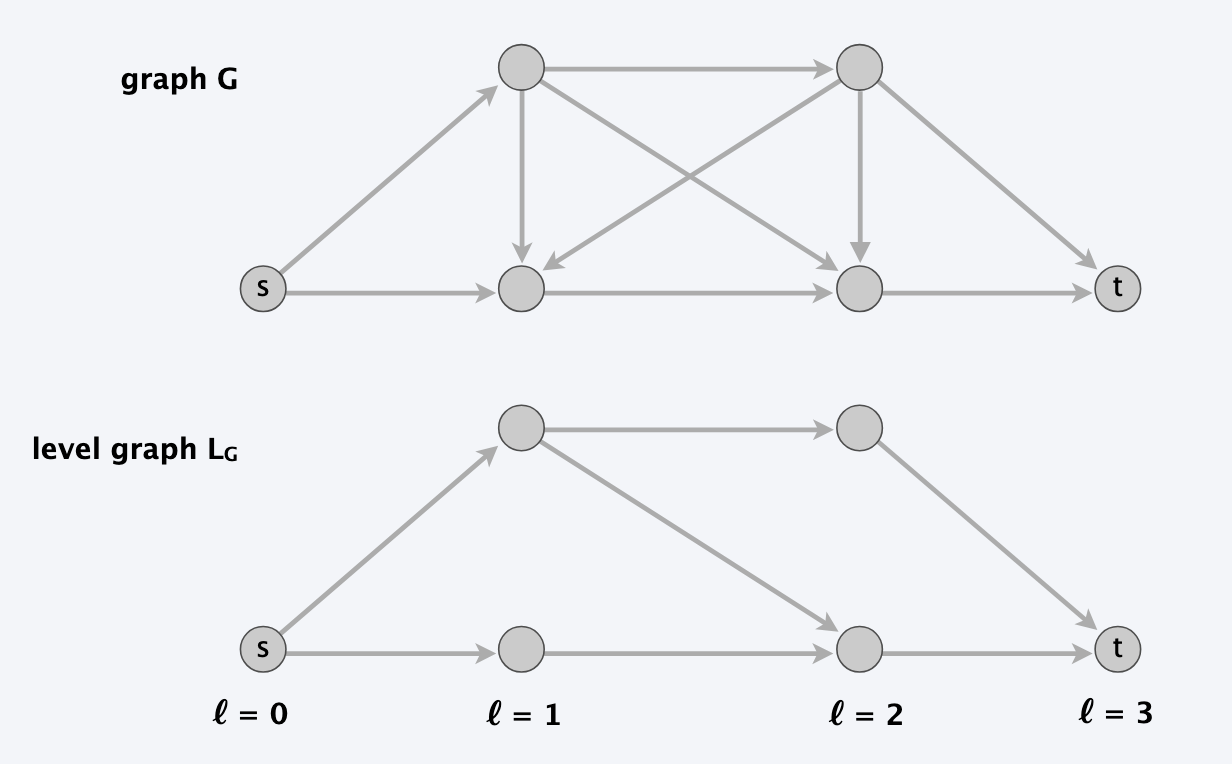
\includegraphics[width=0.5\textwidth]{imm/Screenshot 2026-04-16 alle 17.04.11.png}
\end{figure}\subsection*{Analysis}

\begin{itemize}
    \item \textbf{L1. The shortest path length never decreases.}
    Let $f$ and $f'$ be the flows before and after an augmentation, and
    let $L$, $L'$ be the corresponding level graphs. When we augment along
    a shortest path, the only new edges added to $G_{f'}$ are
    \emph{backward} edges (reversals of edges used). A backward edge
    $(w, v)$ goes from a higher level to a lower level, so any path using
    it is strictly longer than the current shortest path. Therefore the
    shortest path length in $G_{f'}$ is at least that in $G_f$.

    \item \textbf{L2. After at most $m$ augmentations, the shortest path
    strictly increases.}
    Each augmentation saturates at least one edge --- the bottleneck ---
    which is then removed from $L_G$. The only new edges added to $L_G$
    are backward edges, which go in the wrong direction and cannot be part
    of a shortest path of the same length. Therefore, after at most $m$
    augmentations, all edges at the current length are exhausted and the
    shortest path must strictly increase.
\end{itemize}

\begin{theorem}
The shortest augmenting path algorithm runs in $O(m^2 n)$ time.
\end{theorem}

\begin{proof}
\begin{itemize}
    \item Each BFS to find a shortest augmenting path takes $O(m + n)$
    time.
    \item By L2, there are at most $m$ augmentations for each fixed path
    length.
    \item By L1, the path length can increase at most $n - 1$ times
    (it starts at 1 and is at most $n - 1$).
    \item Total augmentations: $O(m \cdot n)$.
    \item Total time: $O(mn) \cdot O(m + n) = O(m^2 n)$.
\end{itemize}
\end{proof}

\paragraph{Remark.}
The bound $O(m^2 n)$ can be improved. By explicitly maintaining the level
graph and processing all augmentations at the same length together
(\textbf{blocking flow}), one phase takes $O(mn)$ time instead of $O(m^2)$,
giving \textbf{Dinic's algorithm} with total running time $O(mn^2)$.
Using dynamic trees (Sleator--Tarjan, 1983), this further improves to
$O(mn \log n)$.

%------------------------------------------------------------
\section{Unit-Capacity Simple Networks}

A network is \textbf{unit-capacity simple} if every edge has capacity 1, and
every non-source, non-sink node has either at most one entering edge or at
most one leaving edge. Bipartite matching graphs are an important example.
\begin{figure}[H]
    \centering
    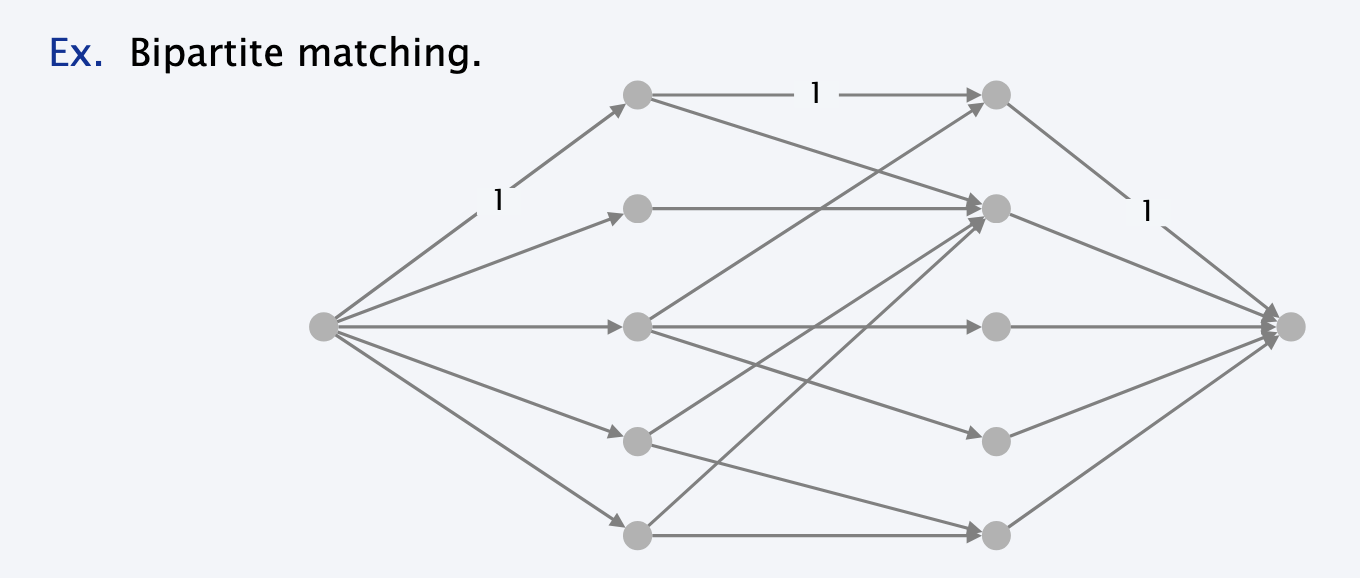
\includegraphics[width=0.5\textwidth]{imm/Screenshot 2026-04-16 alle 17.10.20.png}
\end{figure}
\subsubsection*{Faster Analysis for This Special Case}

\begin{theorem}[Even--Tarjan, 1975]
In unit-capacity simple networks, the shortest augmenting path algorithm
computes a max-flow in $O(m \sqrt{n})$ time.
\end{theorem}

The proof uses three lemmas:
\begin{itemize}
    \item \textbf{L1.} Each phase of normal augmentations takes $O(m)$ time.
    \item \textbf{L2.} After at most $\sqrt{n}$ phases, $f^* - f \leq
    \sqrt{n}$. After $\sqrt{n}$ phases the shortest path has length $>
    \sqrt{n}$, so the level graph has more than $\sqrt{n}$ layers. By a
    pigeonhole argument, some layer $V_h$ has at most $\sqrt{n}$ nodes,
    giving a cut of capacity $\leq \sqrt{n}$.
    \item \textbf{L3.} After at most $\sqrt{n}$ additional augmentations
    (one unit each), the flow is optimal.
\end{itemize}

Combining: $O(\sqrt{n})$ phases $\times$ $O(m)$ per phase $+$ $O(\sqrt{n}
\cdot m)$ final augmentations $= O(m\sqrt{n})$.

\subsubsection*{Application to Bipartite Matching}

Since bipartite matching graphs are unit-capacity simple networks, the
shortest augmenting path algorithm solves bipartite matching in
$O(m\sqrt{n})$ time. This matches the bound of the
\textbf{Hopcroft--Karp algorithm} (1973).

% -------------------------------------------------------------------

\section{Bipartite Matching}

A \textbf{matching} in a graph $G = (V, E)$ is a subset of edges $M \subseteq E$
such that each node appears in at most one edge. A graph is \textbf{bipartite}
if the nodes can be split into two sets $L$ and $R$ so that every edge goes
from $L$ to $R$. The goal of bipartite matching is to find a matching of
maximum cardinality.
\begin{figure}[H]
    \centering
    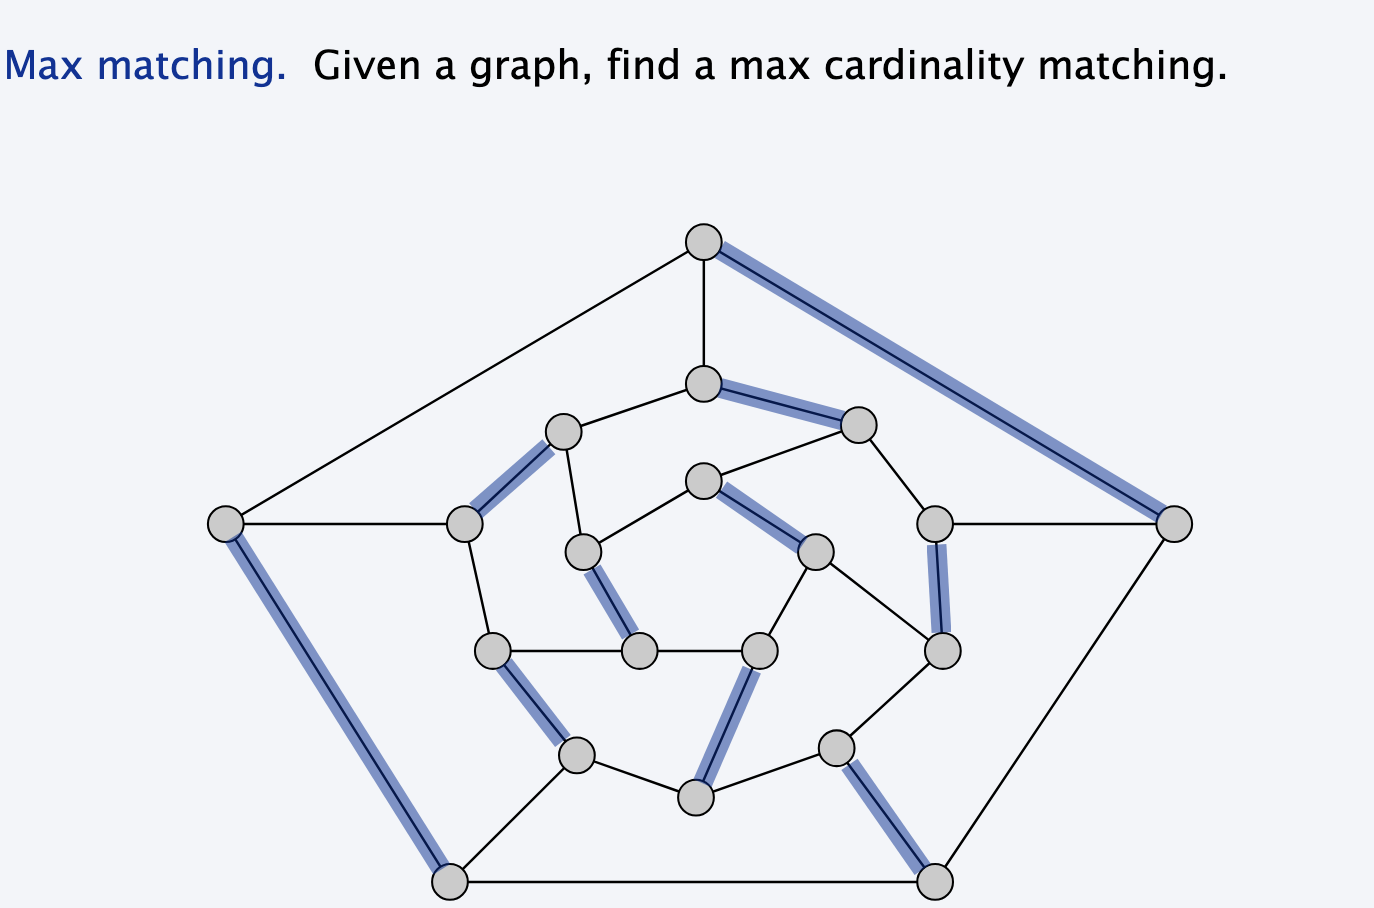
\includegraphics[width=0.5\textwidth]{imm/Screenshot 2026-04-16 alle 17.13.28.png}
\end{figure}
\subsection{Reduction to Max Flow}

Build a directed graph $G'$ as follows:
\begin{itemize}
    \item Direct all edges from $L$ to $R$ with capacity 1.
    \item Add a source $s$ with unit capacity edges to every node in $L$.
    \item Add a sink $t$ with unit capacity edges from every node in $R$.
\end{itemize}

\begin{theorem}
The maximum cardinality of a matching in $G$ equals the value of the
maximum flow in $G'$.
\end{theorem}
\begin{figure}[H]
    \centering
    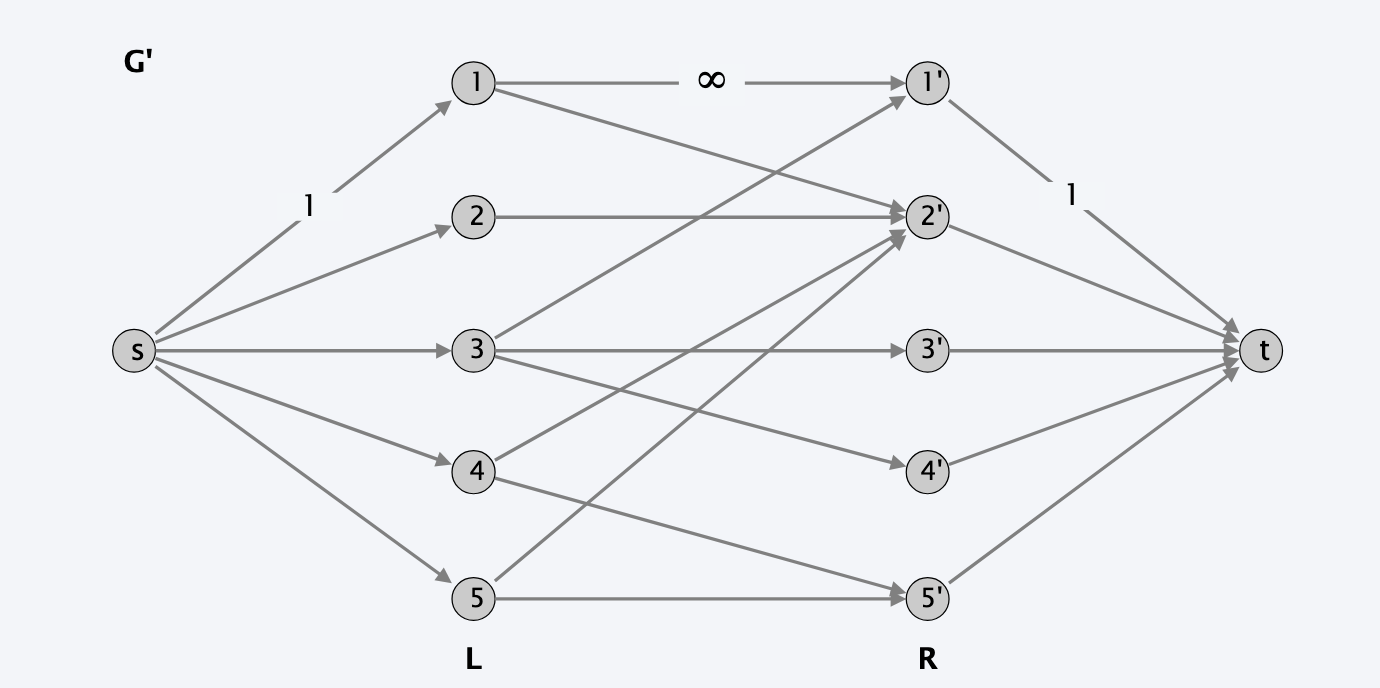
\includegraphics[width=0.5\textwidth]{imm/Screenshot 2026-04-16 alle 17.14.58.png}
\end{figure}
\begin{proof}
\textbf{(Flow $\Rightarrow$ Matching).} Let $f$ be a maximum flow in $G'$. Since all capacities are 1, the integrality theorem guarantees an integer-valued max flow. The edges with $f(e) = 1$ form a matching in $G$ of size $\mathrm{val}(f)$, since each node can have at most one unit of flow passing through it.
\textbf{(Matching $\Rightarrow$ Flow).} Let $M$ be a maximum matching in $G$. We can construct a flow $f$ in $G'$ by sending 1 unit of flow along the path $s \to u \to v \to t$ for each edge $(u, v) \in M$. This flow has value equal to the size of the matching, $\mathrm{val}(f) = |M|$.
\end{proof}

\subsection{Hall's Theorem}

A \textbf{perfect matching} is a matching where every node appears in
exactly one edge. For a bipartite graph with $|L| = |R|$, a perfect matching
exists if and only if for every subset $S \subseteq L$, the set of neighbors
$N(S)$ satisfies $|N(S)| \geq |S|$. This is \textbf{Hall's theorem}.
\begin{figure}[H]
    \centering
    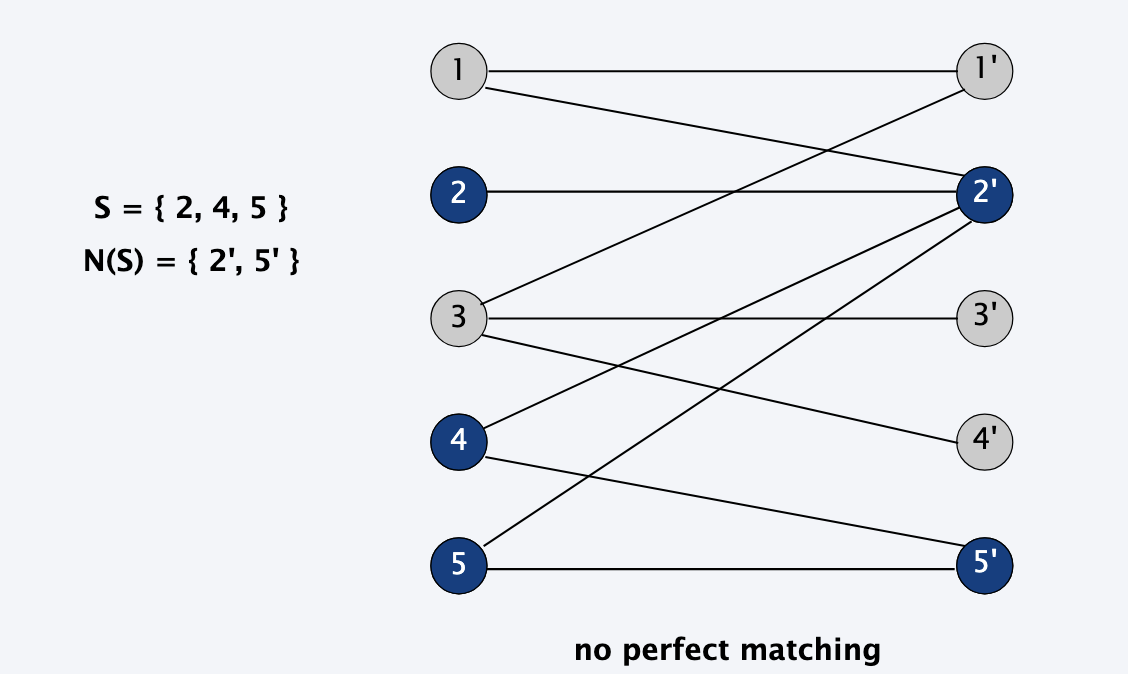
\includegraphics[width=0.5\textwidth]{imm/Screenshot 2026-04-16 alle 17.36.27.png}
    \caption{in this case, we choose as S=2,4,5 and N(S)={2,5}; so |N(S)|=2<|S|=3, for this reason, is impossible to find a perfect matching
    }
\end{figure}

\begin{theorem}[Hall, 1935]
A bipartite graph $G = (L \cup R,\, E)$ with $|L| = |R|$ has a perfect
matching if and only if $|N(S)| \geq |S|$ for all $S \subseteq L$.
\end{theorem}

As a corollary, every $k$-regular bipartite graph has a perfect matching,
since the flow $f(u,v) = 1/k$ on each edge is a feasible flow of value $|L|$.

%------------------------------------------------------------
\subsection{Edge-Disjoint Paths}

Two paths are \textbf{edge-disjoint} if they share no edge in common. 
\newline
The problem is:
given a digraph $G$ and two nodes $s$ and $t$, find the maximum number of
edge-disjoint $s$-$t$ paths.

\begin{figure}[H]
    \centering
    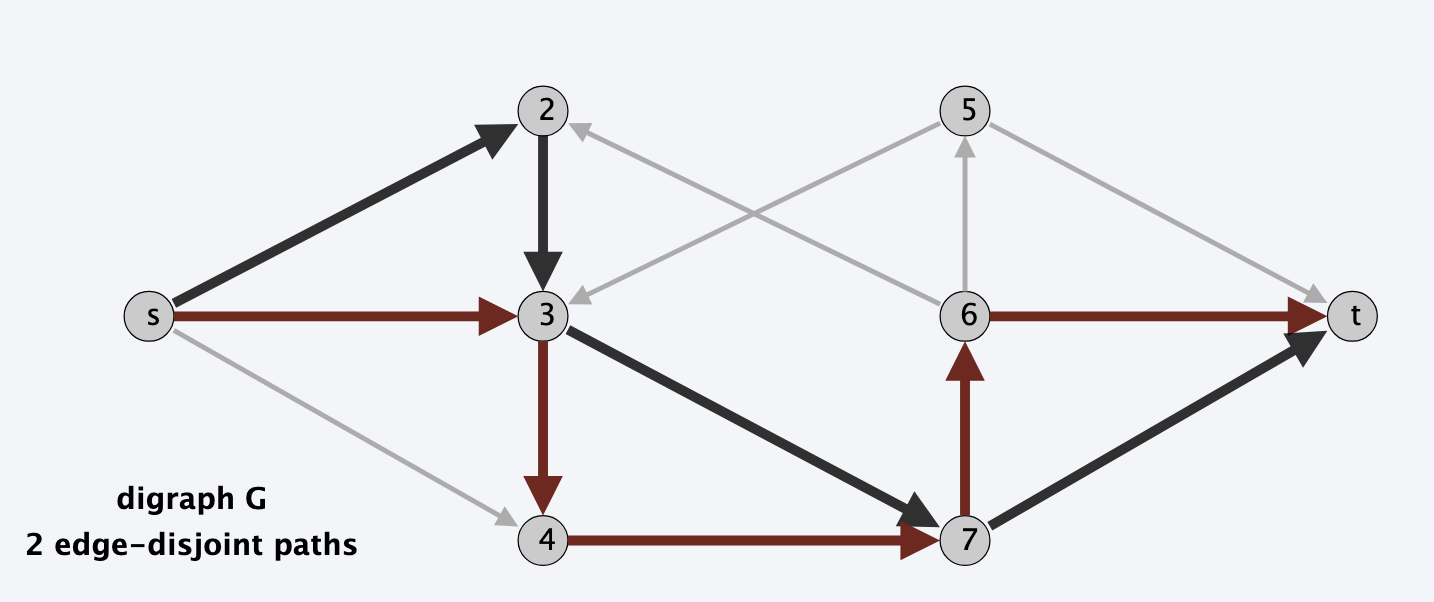
\includegraphics[width=0.5\textwidth]{imm/Screenshot 2026-04-16 alle 17.57.18.png}
\end{figure}

\subsection{Reduction to Max Flow}

Assign unit capacity to every edge. Then:

\begin{theorem}
The maximum number of edge-disjoint $s$-$t$ paths equals the value of the
maximum flow.
\end{theorem}

\begin{proof}
\textbf{(Flow $\Rightarrow$ Paths).} Let $f$ be a maximum flow. By the integrality theorem, there exists a maximum flow $f^*$ where every flow value is an integer (0 or 1). The edges with $f^*(e) = 1$ form a collection of edge-disjoint $s$-$t$ paths, since each node can have at most one unit of flow passing through it.
\textbf{(Paths $\Rightarrow$ Flow).} Let $P_1, \ldots, P_k$ be a maximum collection of edge-disjoint $s$-$t$ paths. We can construct a flow $f$ by sending 1 unit of flow along each path $P_i$. This flow has value $k$, which is the number of edge-disjoint paths.
\end{proof}

A direct consequence is \textbf{Menger's theorem}: the maximum number of
edge-disjoint $s$-$t$ paths equals the minimum number of edges whose removal
disconnects $t$ from $s$.

For \textbf{undirected} graphs, replace each undirected edge with two
antiparallel directed edges of capacity 1. There always exists a maximum flow
where at most one of each antiparallel pair carries flow, so the same result
holds.

\subsection{Circulation with Demands}

A \textbf{circulation} is a generalization of flow where each node $v$ has a
demand $d_v$: a positive $d_v$ means $v$ needs to receive $d_v$ more units
than it sends, and a negative $d_v$ means $v$ produces flow.

A feasible circulation satisfies:
\begin{itemize}
    \item \textbf{Capacity}: $0 \leq f(e) \leq c_e$ for each edge $e$.
    \item \textbf{Conservation}: $\sum_{e \text{ into } v} f(e) - \sum_{e
    \text{ out of } v} f(e) = d_v$ for each node $v$.
\end{itemize}
\begin{figure}[H]
    \centering
    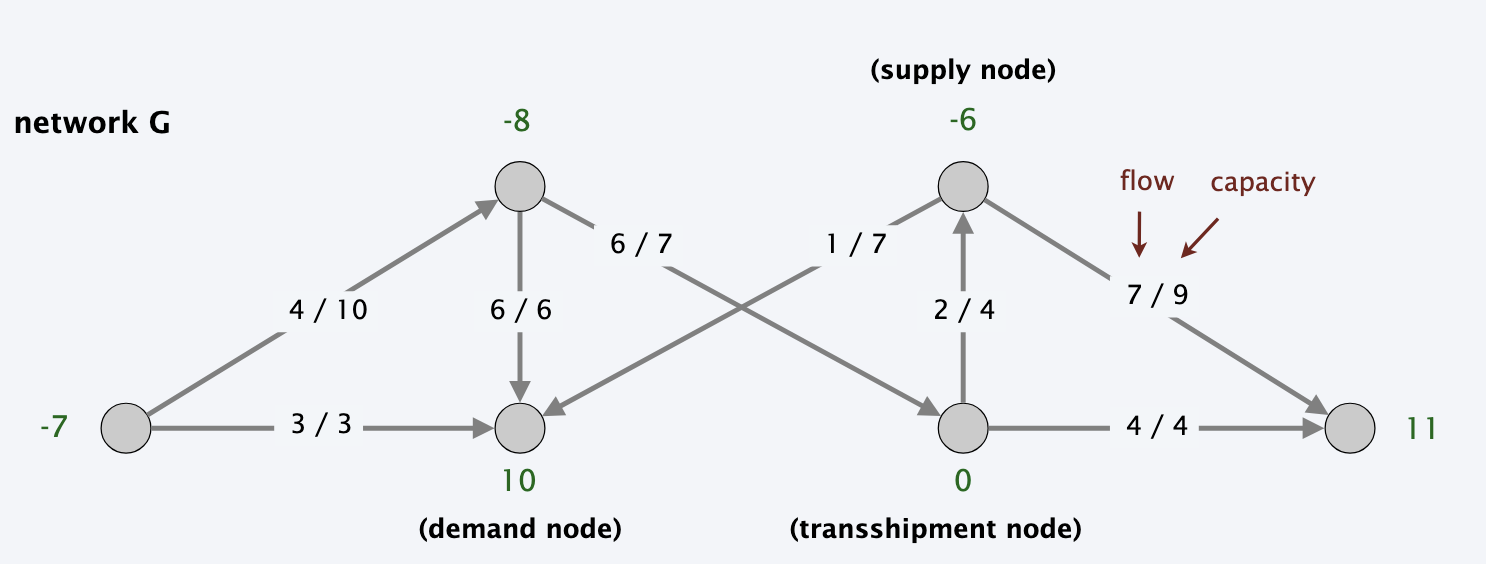
\includegraphics[width=0.5\textwidth]{imm/Screenshot 2026-04-16 alle 18.11.41.png}
\end{figure}

\subsubsection{Reduction to Max Flow}

Add a super-source $s^*$ and super-sink $t^*$:
\begin{itemize}
    \item For each node $v$ with $d_v > 0$, add edge $(s^*, v)$ with capacity
    $d_v$.
    \item For each node $v$ with $d_v < 0$, add edge $(v, t^*)$ with capacity
    $-d_v$.
\end{itemize}

A feasible circulation exists if and only if the max flow in this new graph
saturates all edges leaving $s^*$.



\begin{figure}[H]
    \centering
    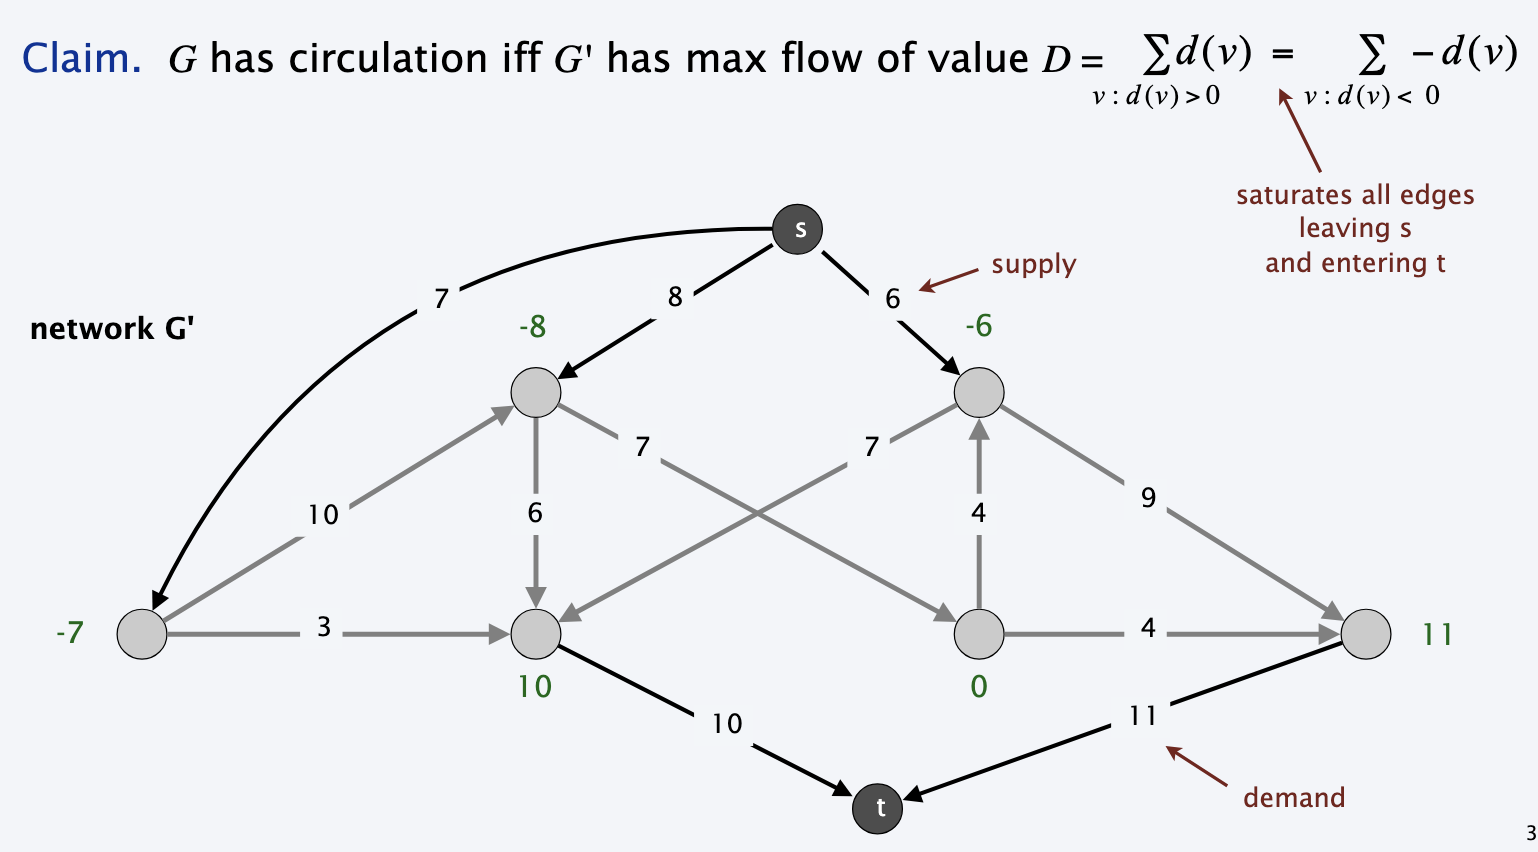
\includegraphics[width=0.5\textwidth]{imm/Screenshot 2026-04-16 alle 18.12.57.png}
\end{figure}
\begin{theorem}
    Integrality theorem: if all capacities and demands are integers, then there exists a feasible circulation where every flow value is an integer.
\end{theorem}

\begin{theorem}[Cut certificate of infeasibility]
Given a circulation instance $(V,E,c,d)$, no feasible circulation exists if
there is a partition $(A,B)$ of $V$ such that
\[
    \sum_{v \in B} d_v > \operatorname{cap}(A,B),
\]
where
\[
    \operatorname{cap}(A,B) = \sum_{\substack{(u,v)\in E\\u\in A,\ v\in B}} c_{uv}.
\]
\end{theorem}

\subsection{Lower Bounds}

Edges can also have a \textbf{lower bound} $\ell_e$: the flow must satisfy
$\ell_e \leq f(e) \leq c_e$. This can be reduced to the standard circulation
problem by sending $\ell_e$ units along each edge in advance and updating
the demands of both endpoints accordingly.
\newline
A \textbf{circulation} with lower bounds is a flow that satisfies :
\begin{itemize}
    \item \textbf{Capacity}: $\ell_e \leq f(e) \leq c_e$ for each edge $e$.
    \item \textbf{Conservation}: $\sum_{e \text{ into }v} f(e) - \sum_{e \text{ out of } v} f(e) = d_v$ for each node $v$.
\end{itemize}

\textbf{Simple idea.} First, satisfy all lower bounds in advance: send
$\ell_e$ units on every edge $e$. Then only the \emph{extra} flow is unknown.

Define:
\[
    f'(e)=f(e)-\ell_e.
\]
So in the transformed network $G'$:
\begin{itemize}
    \item each edge has residual capacity interval
    $0 \leq f'(e) \leq c_e-\ell_e$;
    \item node demands must be updated because of the pre-sent flow:
    \[
        d'_v = d_v + \sum_{e\text{ out of }v} \ell_e
              - \sum_{e\text{ into }v} \ell_e.
    \]
\end{itemize}
\begin{figure}[H]
    \centering
    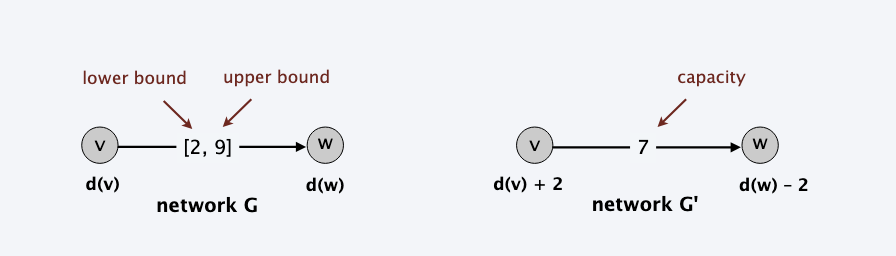
\includegraphics[width=0.7\textwidth]{imm/Screenshot 2026-04-16 alle 18.36.01.png}
\end{figure}

\begin{theorem}[Reduction for lower bounds]
There exists a feasible circulation in $G$ (with bounds
$\ell_e \le f(e) \le c_e$) if and only if there exists a feasible
circulation in the transformed instance $G'$ (with bounds
$0 \le f'(e) \le c_e-\ell_e$ and demands $d'_v$). Moreover, if all data are
integers, then a feasible circulation can be chosen integer-valued.
\end{theorem}

\begin{proof}[Proof sketch]
Set $f'(e)=f(e)-\ell_e$ (equivalently, $f(e)=f'(e)+\ell_e$).

The capacity constraints are exactly the same information written in two
different ways:
\[
    \ell_e \le f(e) \le c_e
    \iff
    0 \le f'(e) \le c_e-\ell_e.
\]

At each node $v$, replace $f$ with $f'+\ell$ in flow conservation. This gives
the new demand equation with $d'_v$. So feasibility in $G$ and feasibility in
$G'$ are equivalent.

If capacities, demands, and lower bounds are integers, then $G'$ has an
integer feasible circulation (integrality theorem). Adding back $\ell_e$ keeps
everything integer, so $G$ also has an integer feasible circulation.
\end{proof}

 
%------------------------------------------------------------
\section{Survey Design}

A company wants to survey $n_1$ consumers about $n_2$ products. Consumer $i$
can only be asked about product $j$ if they own it. Each consumer $i$ must
be asked between $c_i^-$ and $c_i^+$ questions, and each product $j$ must
receive between $p_j^-$ and $p_j^+$ responses.

This is modeled as a \textbf{circulation problem with lower bounds}:
\begin{itemize}
    \item Add an edge $(i, j)$ if consumer $i$ owns product $j$.
    \item Add edges from $s$ to each consumer and from each product to $t$,
    with lower and upper bounds given by the constraints.
    \item Add a return edge from $t$ to $s$.
\end{itemize}

A feasible integer circulation corresponds to a valid survey design.

%------------------------------------------------------------
\section{Airline Scheduling}

The goal is to manage a set of $k$ flights using the minimum number of crews.
A crew can move from flight $i$ to flight $j$ if $j$ is reachable after $i$
ends (same or nearby airport, enough time).

This is modeled as a \textbf{circulation problem}:
\begin{itemize}
    \item For each flight $i$, add nodes $u_i$ (departure) and $v_i$
    (arrival) with edge $(u_i, v_i)$ of lower bound and capacity 1.
    \item If a crew can go from flight $i$ to flight $j$, add edge
    $(v_i, u_j)$ with capacity 1.
    \item Add source $s$ and sink $t$ to control the total number of crews.
\end{itemize}
\begin{figure}[H]
    \centering
    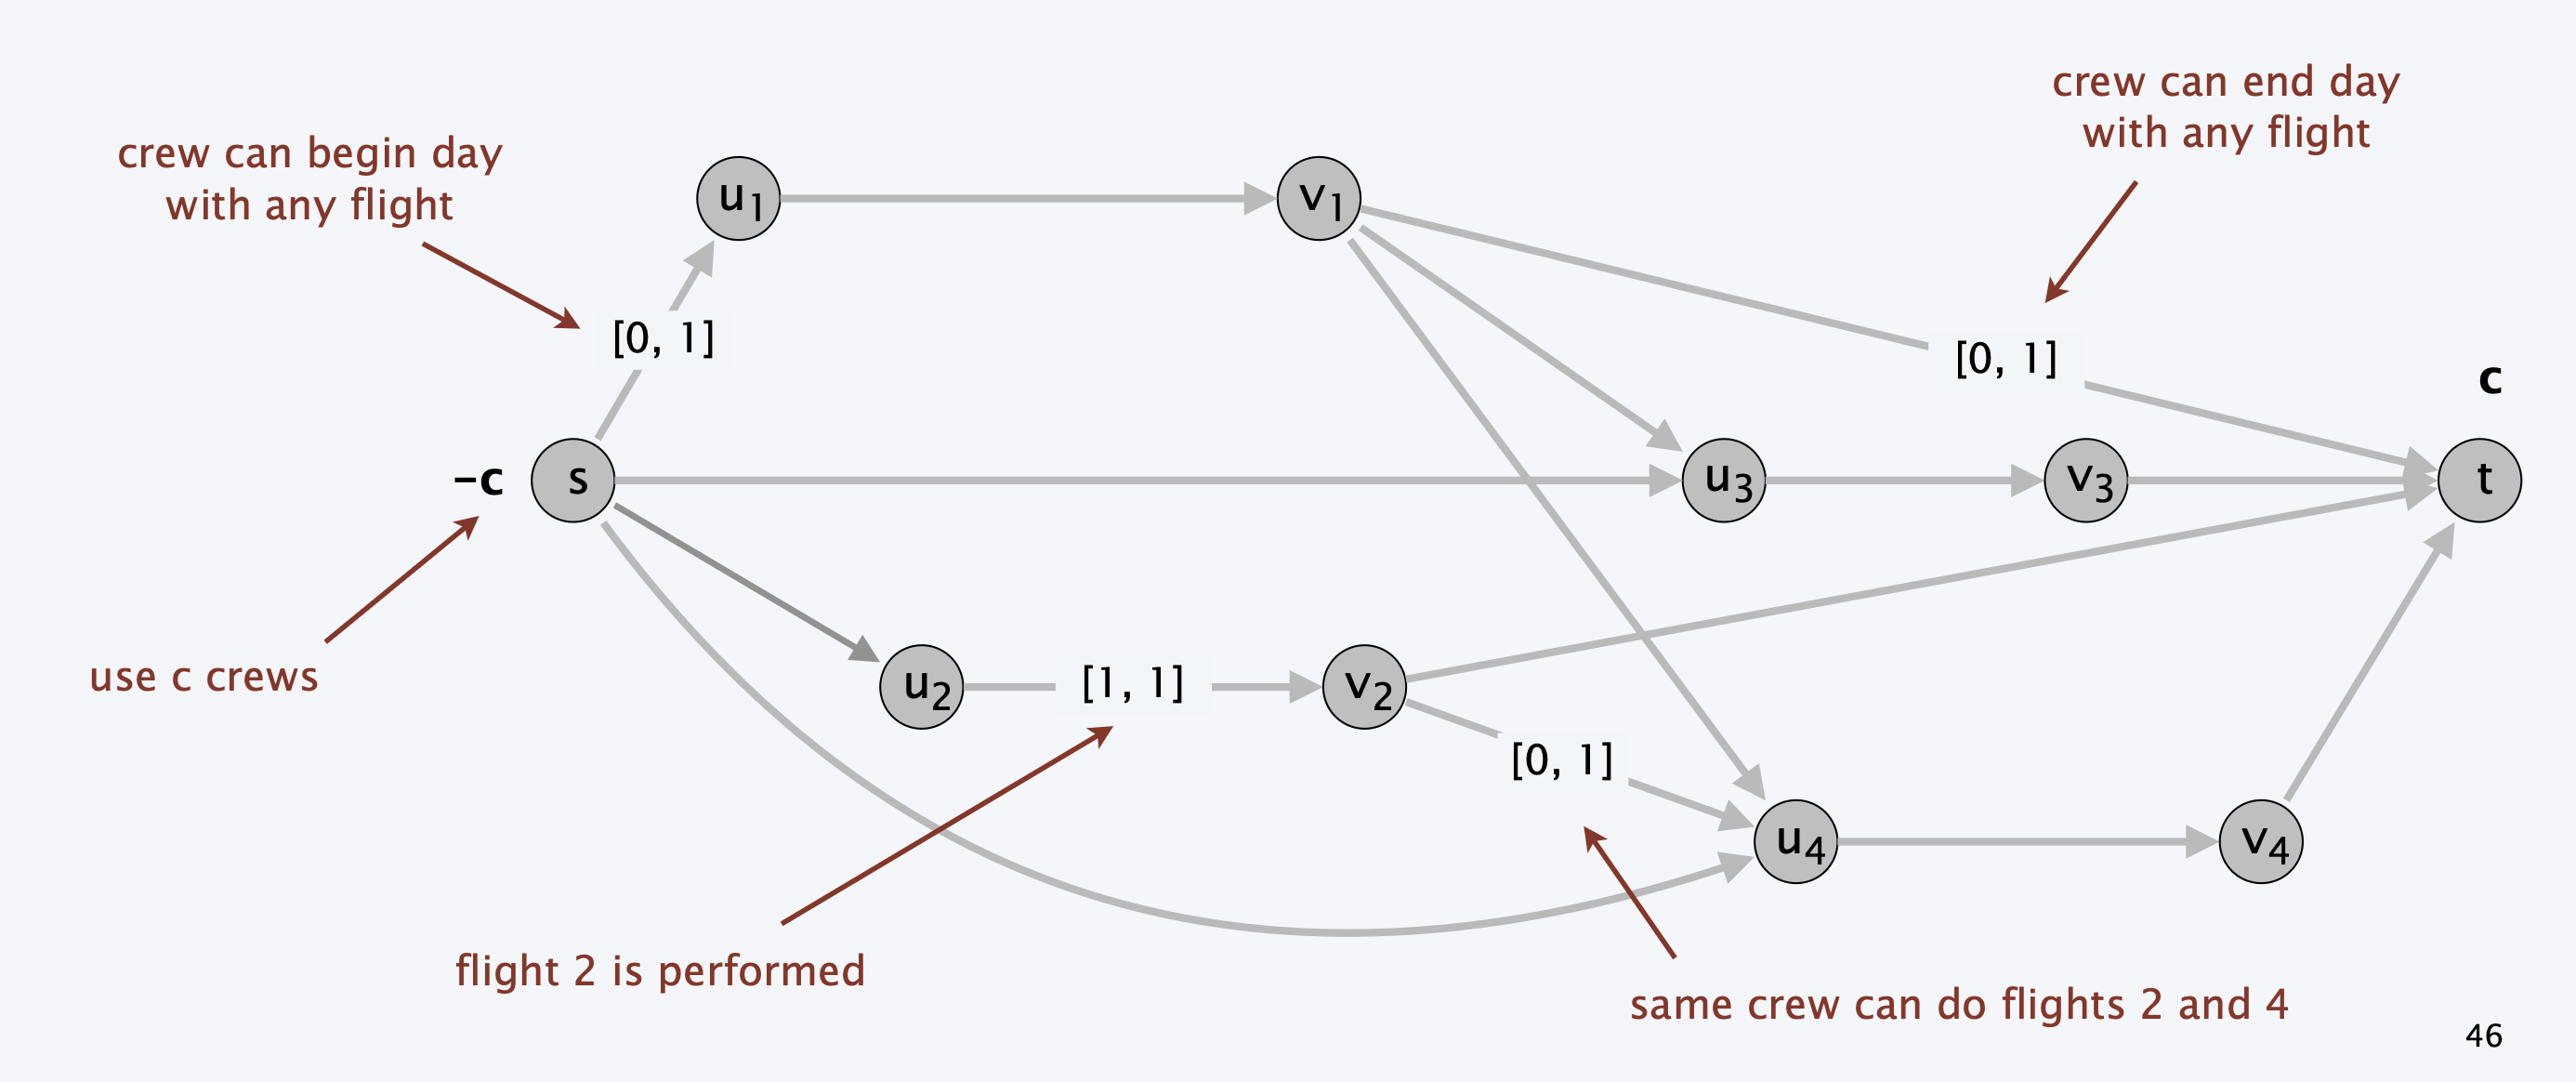
\includegraphics[width=0.7\textwidth]{imm/Screenshot 2026-04-17 alle 13.13.03.png}
\end{figure}
\begin{theorem}
The airline scheduling problem can be solved in $O(k^3 \log k)$ time,
using binary search on the number of crews and solving $O(\log k)$
circulation problems.
\end{theorem}

%------------------------------------------------------------
\subsection{Project Selection}

Each project $v$ has a revenue $p_v$ (which can be negative, representing a
cost). Some projects require others: if project $v$ requires project $w$, then
$v$ cannot be chosen without also choosing $w$. The goal is to find a feasible
subset of projects that maximizes total revenue.
\textbf{prerequisite edges} $(v, w)$ indicate that $v$ requires $w$.
\begin{figure}[H]
    \centering
    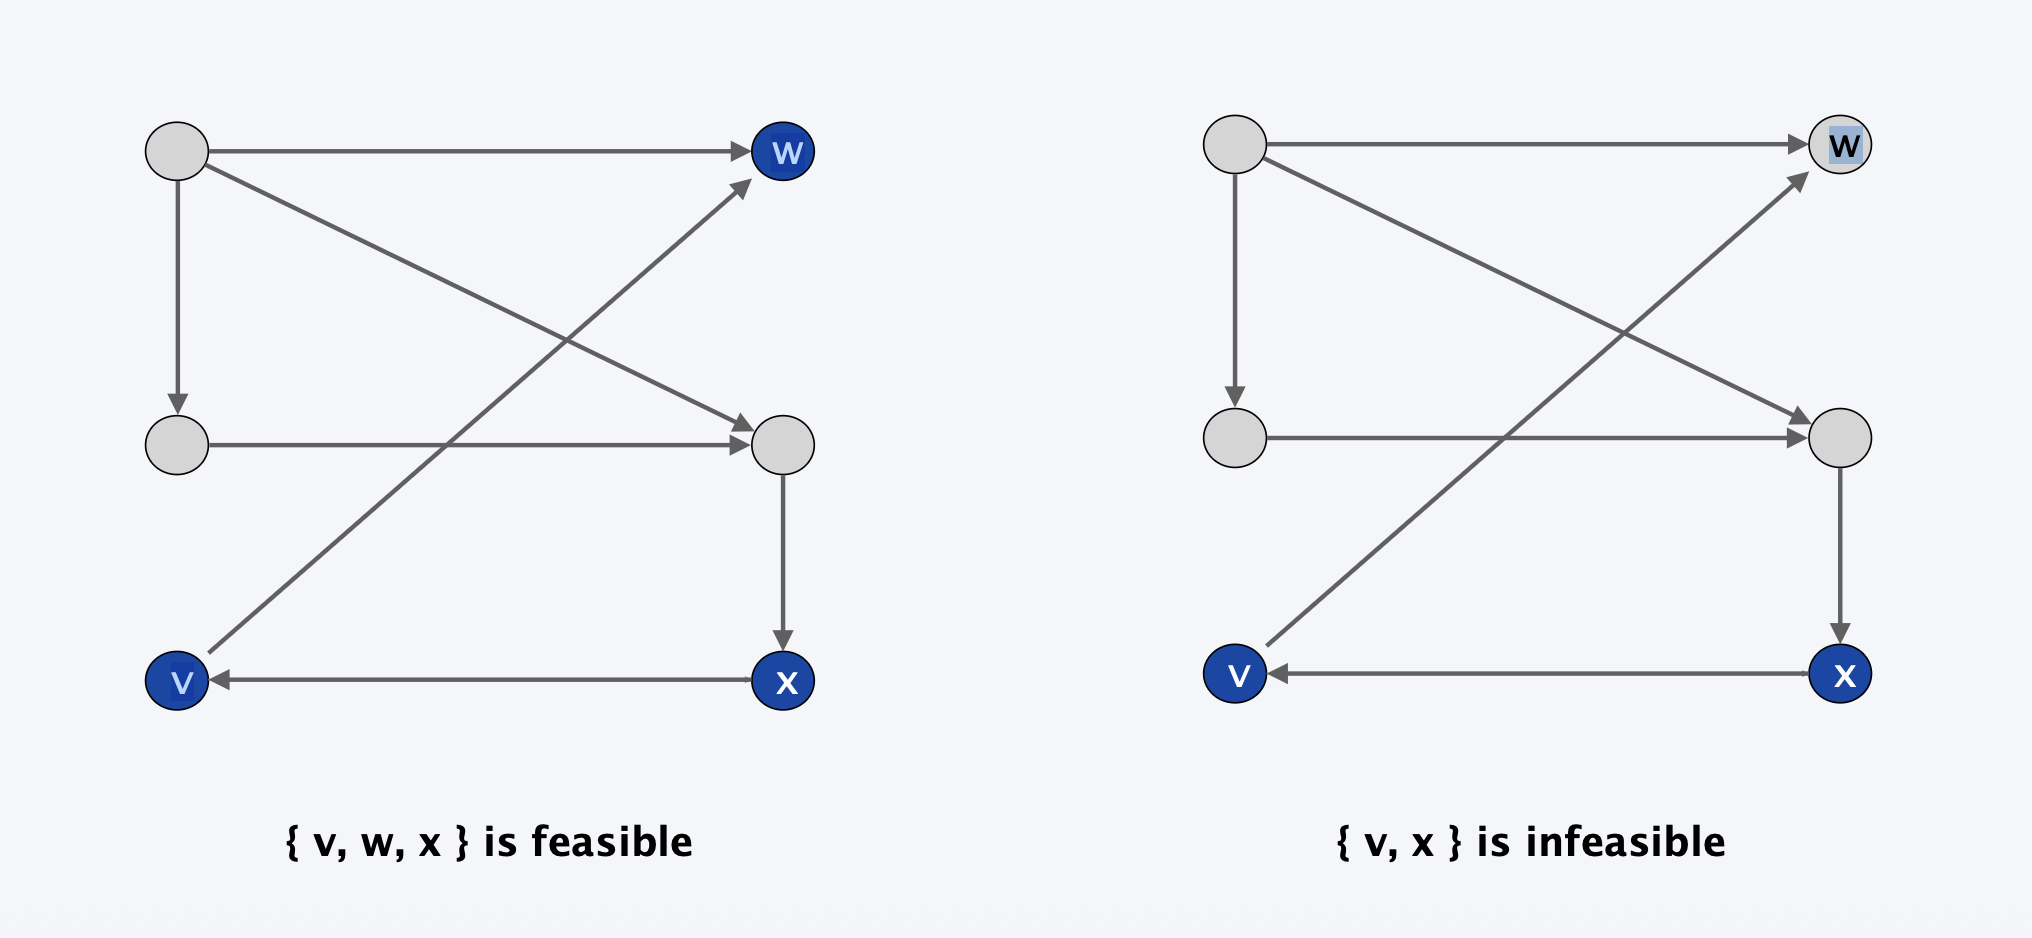
\includegraphics[width=0.5\textwidth]{imm/Screenshot 2026-04-17 alle 13.14.51.png}
\end{figure}
\subsubsection*{Reduction to Min Cut}

Build a graph $G'$:
\begin{itemize}
    \item For each prerequisite edge $(v, w)$, add an edge with
    $\infty$ capacity.
    \item For each project $v$ with $p_v > 0$, add edge $(s, v)$ with
    capacity $p_v$.
    \item For each project $v$ with $p_v < 0$, add edge $(v, t)$ with
    capacity $-p_v$.
\end{itemize}

The infinite capacity edges ensure that the selected set is always feasible.
The minimum cut in $G'$ gives the maximum revenue subset.
\begin{figure}[H]
    \centering
    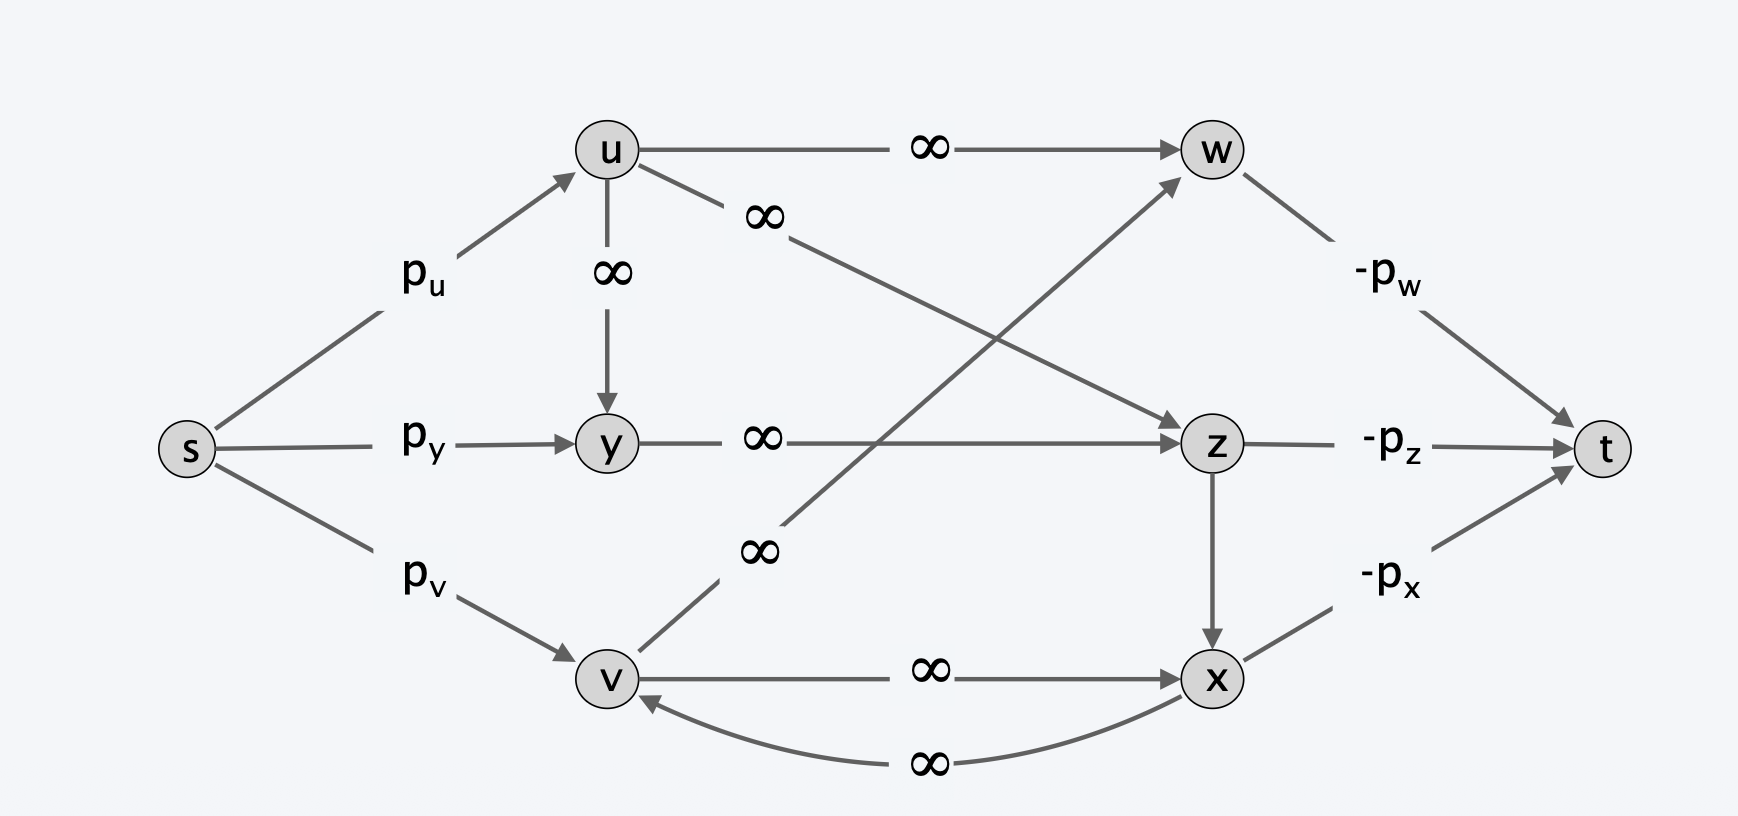
\includegraphics[width=0.5\textwidth]{imm/Screenshot 2026-04-17 alle 13.15.49.png}
\end{figure}
\chapter{ exercises on Network Flow}
\begin{figure}[H]
    \centering
    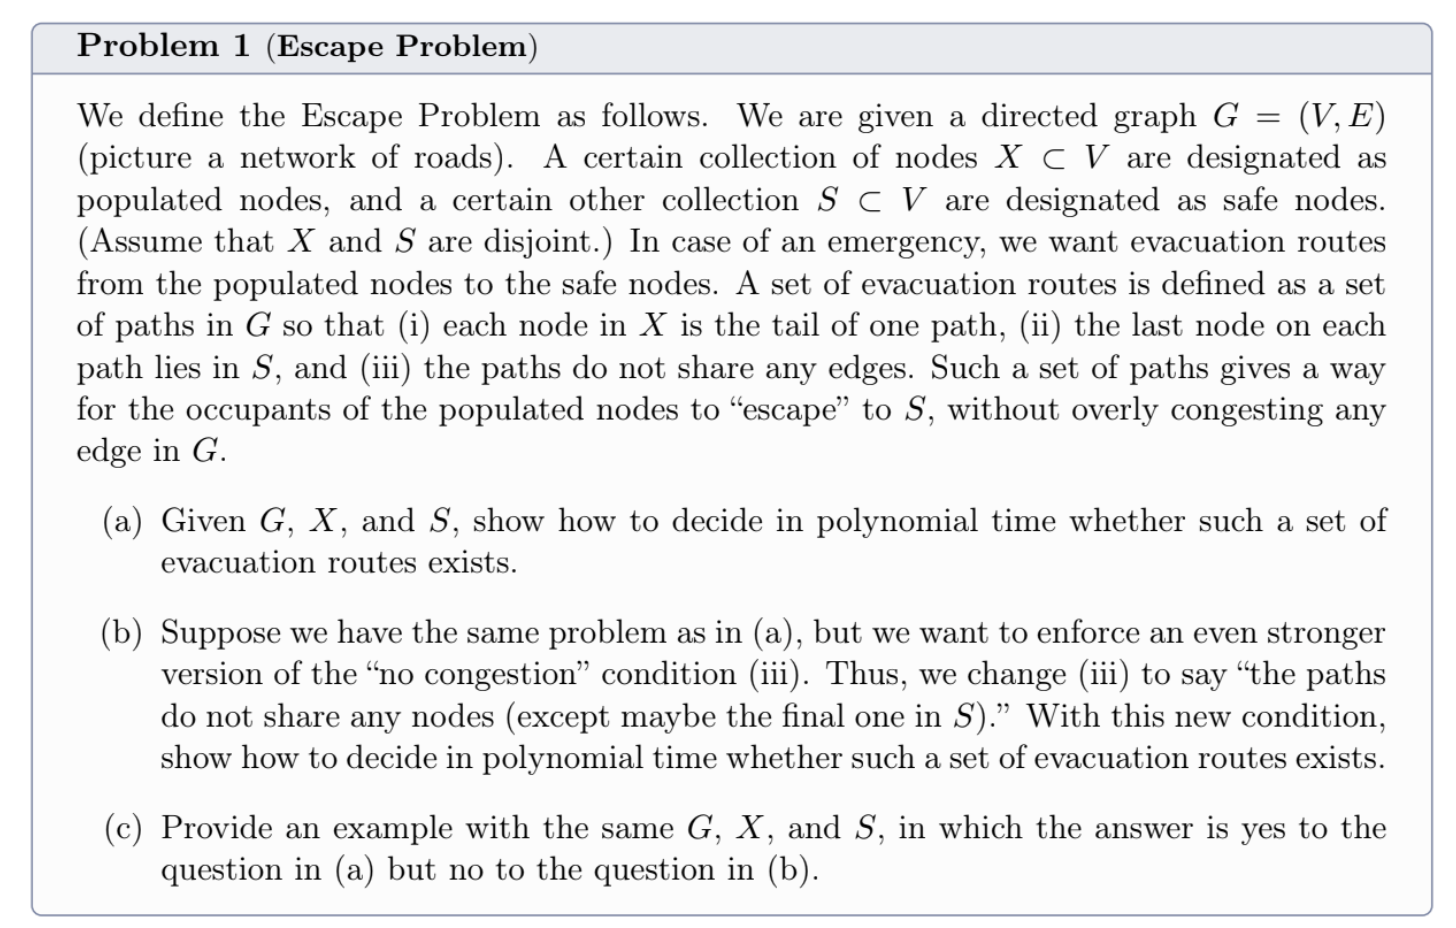
\includegraphics[width=1\textwidth]{imm/Screenshot 2026-04-16 alle 14.31.29.png}  
\end{figure}

%------------------------------------------------------------
\subsection*{Part (i): Edge-Disjoint Evacuation Routes}

\paragraph{Construction of $G'$.}
We build a flow network $G' = (V', E')$ as follows:
\begin{itemize}
    \item \textbf{Source edges:} For each $u \in X$, add edge $(s, u)$
    with capacity $c(s, u) = 1$.
 \item \textbf{Sink edges:} For each $v \in S$, add edge $(v, t)$
with capacity $c(v, t) = |X|$ . Multiple evacuation
routes are allowed to end at the same safe node, so we do not
restrict the flow entering $t$ from $S$.
    \item \textbf{Internal edges:} For every original edge $e \in E$,
    keep it with capacity $c(e) = 1$.
\end{itemize}
\begin{figure}[H]
    \centering
    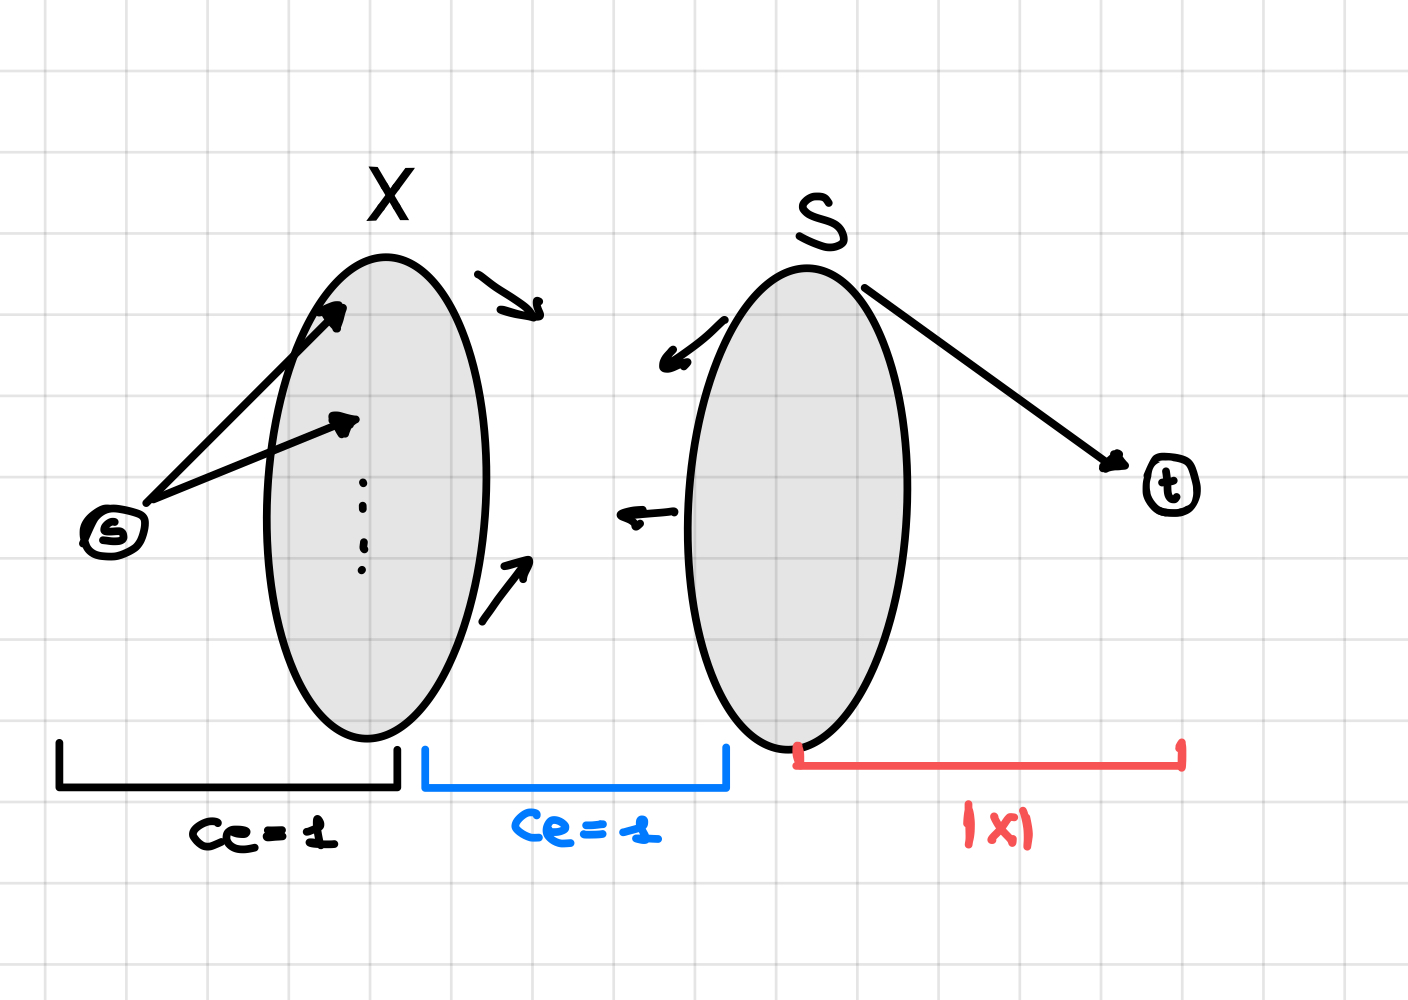
\includegraphics[width=0.5\textwidth]{imm/Immagine JPEG-4502-AD33-DC-0.jpeg}
\end{figure}


A valid set of evacuation routes exists if and only if $\mathrm{maxflow} =
|X|$.

\begin{proof}
We prove both directions.

\medskip
\noindent $(\Rightarrow)$ Given $|X|$ edge-disjoint paths, set $f(e) = 1$
if edge $e$ is used by some path and $f(e) = 0$ otherwise. Edge-disjointness
ensures all capacity constraints hold. Since one path leaves each $u \in X$,
the edge $(s, u)$ is saturated for all $u \in X$, so $\mathrm{val}(f) =
|X|$.

\medskip
\noindent $(\Leftarrow)$ If the max-flow equals $|X|$, all edges $(s, u)$
for $u \in X$ are saturated, so one unit of flow leaves each populated node.
By flow conservation and the fact that all capacities are 1, each unit of
flow travels along a distinct path from some $u \in X$ to some $v \in S$.
Since each edge carries at most 1 unit, these paths are edge-disjoint.
\end{proof}

This construction has $O(|V|)$ nodes and $O(|E|)$ edges, so it runs in
polynomial time.

%------------------------------------------------------------
\subsection*{Part (ii): Node-Disjoint Evacuation Routes}

To enforce that paths do not share any intermediate node, we use the
\textbf{node-splitting technique}.

\paragraph{Construction of $G''$.}
For \textbf{every} node $w \in V$, we replace it with two nodes $w_{\mathrm{in}}$
and $w_{\mathrm{out}}$, connected by a directed edge $(w_{\mathrm{in}},\,
w_{\mathrm{out}})$. The capacity of this internal edge depends on the role of $w$:
\begin{figure}[H]
    \centering
    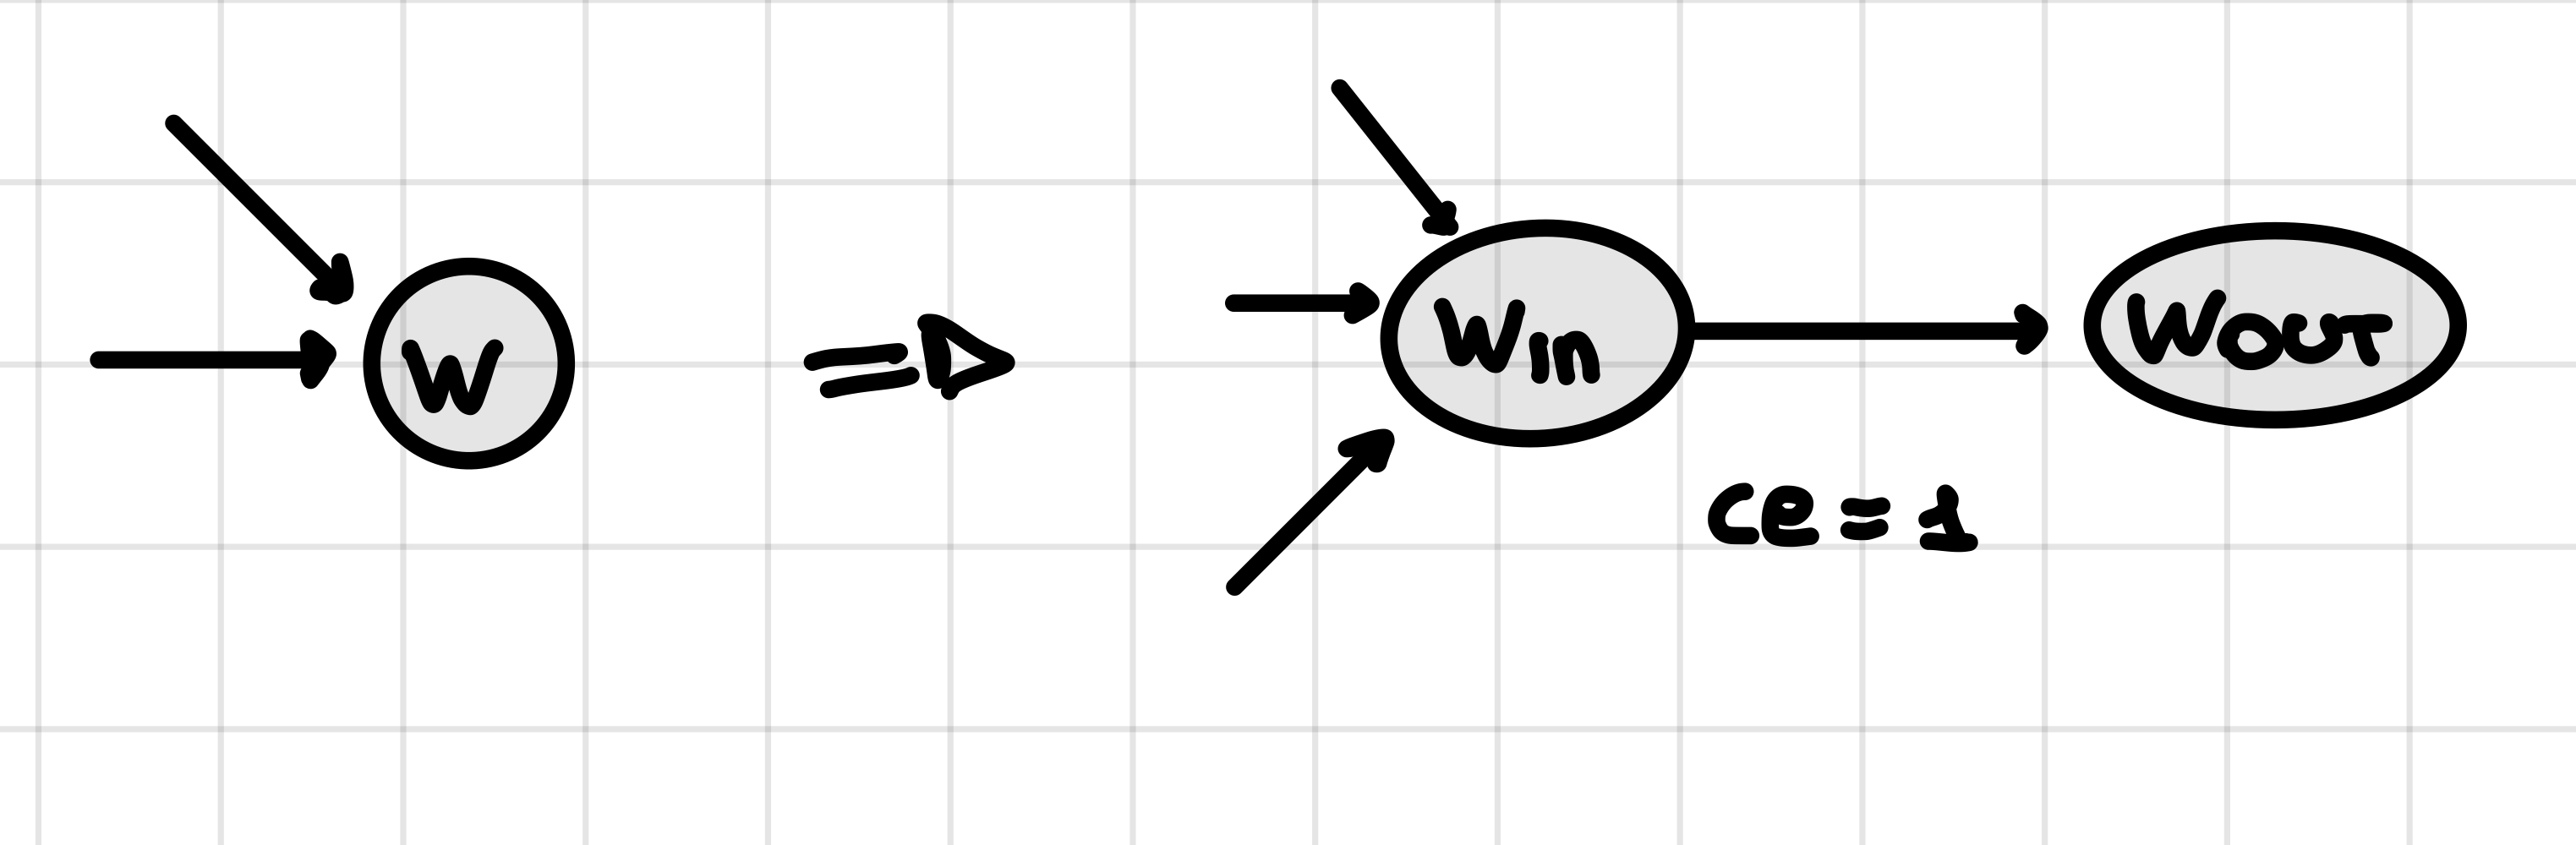
\includegraphics[width=0.5\textwidth]{imm/Immagine JPEG-4D15-AFBC-7B-0.jpeg}
\end{figure}

The remaining edges are built as follows:
\begin{itemize}
    \item \textbf{Internal edges:} Every original edge $(u, v) \in E$ becomes
    an edge $(u_{\mathrm{out}},\, v_{\mathrm{in}})$ with capacity 1.
    \item \textbf{Source edges:} Add a super-source $s$ and, for each $u \in X$,
    add edge $(s,\, u_{\mathrm{in}})$ with capacity 1.
    \item \textbf{Sink edges:} Add a super-sink $t$ and, for each $v \in S$,
    add edge $(v_{\mathrm{out}},\, t)$ with capacity $|X|$ .
\end{itemize}
%------------------------------------------------------------
\subsection*{Part (iii): An Example Where (a) is Yes but (b) is No}

Consider the following graph with $X = \{x_1, x_2\}$,
$S = \{s_1\}$, and a single intermediate node $m$:

\begin{center}
\begin{tikzpicture}[node distance=1.8cm, auto, thick]
  \node (x1) {$x_1$};
  \node (x2) [below of=x1] {$x_2$};
  \node (m)  [right of=x1, yshift=-0.9cm] {$m$};
  \node (s1) [right of=m] {$s_1$};
  \draw[->] (x1) -- (m);
  \draw[->] (x2) -- (m);
  \draw[->] (m)  -- (s1);
\end{tikzpicture}
\end{center}

\noindent Formally: $V = \{x_1, x_2, m, s_1\}$,
$E = \{(x_1, m),\, (x_2, m),\, (m, s_1)\}$,
$X = \{x_1, x_2\}$, $S = \{s_1\}$.

\begin{itemize}
    \item \textbf{Part (a) answer: Yes.} The two paths
    $x_1 \to m \to s_1$ and $x_2 \to m \to s_1$ share the node $m$
    but share \emph{no edge}. So edge-disjoint evacuation routes exist.
    \item \textbf{Part (b) answer: No.} Both paths must pass through $m$
    to reach $s_1$. Since $m$ is the only intermediate node, there is no
    way to route both $x_1$ and $x_2$ to $S$ without sharing $m$.
    The max-flow in $G''$ is 1 (the bottleneck is the single edge
    $m_{\mathrm{in}} \to m_{\mathrm{out}}$ with capacity 1), which is
    less than $|X| = 2$.
\end{itemize}

\subsection* {Problem 3 :Free-Standing Subset}
We are given a set of n countries that are engaged in
trade with one another. For each country i, we have the value si of its budget surplus; this
number may be positive or negative, with a negative number indicating a deficit. For each
pair of countries i, j, we have the total value eij of all exports from i to j; this number is
always nonnegative. We say that a subset S of the countries is free-standing if the sum
of the budget surpluses of the countries in S, minus the total value of all exports from
countries in S to countries not in S, is nonnegative.
Give a polynomial-time algorithm that takes this data for a set ofn countries and decides
whether it contains a nonempty free-standing subset that is not equal to the full set.


Given $n$ countries with budget surpluses $s_i$ and export values $e_{ij}
\geq 0$, a subset $S$ is \emph{free-standing} if
\[
\sum_{i \in S} s_i \;-\; \sum_{\substack{i \in S,\, j \notin S}} e_{ij}
\;\geq\; 0.
\]
Give a polynomial-time algorithm to decide whether a nonempty free-standing
subset $S \subsetneq \{1, \dots, n\}$ exists.

\paragraph{Key Observation.}
We rewrite the free-standing condition. Let $\bar{S} = \{1,\dots,n\}
\setminus S$. A subset $S$ is free-standing iff:
\[
\sum_{i \in S} s_i - \sum_{\substack{i \in S \\ j \in \bar{S}}} e_{ij}
\geq 0
\quad \Longleftrightarrow \quad
\sum_{\substack{i \in S \\ j \in \bar{S}}} e_{ij} \leq \sum_{i \in S} s_i.
\]

\paragraph{Construction of the Flow Network $G'$.}
We reduce the problem to a \textbf{minimum cut} problem. Build a directed
graph $G' = (V', E')$ as follows:
\begin{itemize}
    \item \textbf{Nodes:} One node per country, plus a super-source $s$
    and a super-sink $t$. So $V' = \{1, \dots, n\} \cup \{s, t\}$.

    \item \textbf{Edges between countries:} For each pair $i \neq j$, add
    edge $(i, j)$ with capacity $c(i,j) = e_{ij}$.

    \item \textbf{Source edges:} For each country $i$ with $s_i > 0$, add
    edge $(s, i)$ with capacity $c(s, i) = s_i$.

    \item \textbf{Sink edges:} For each country $i$ with $s_i < 0$, add
    edge $(i, t)$ with capacity $c(i, t) = -s_i$.
\end{itemize}
\begin{figure}[H]
    \centering
    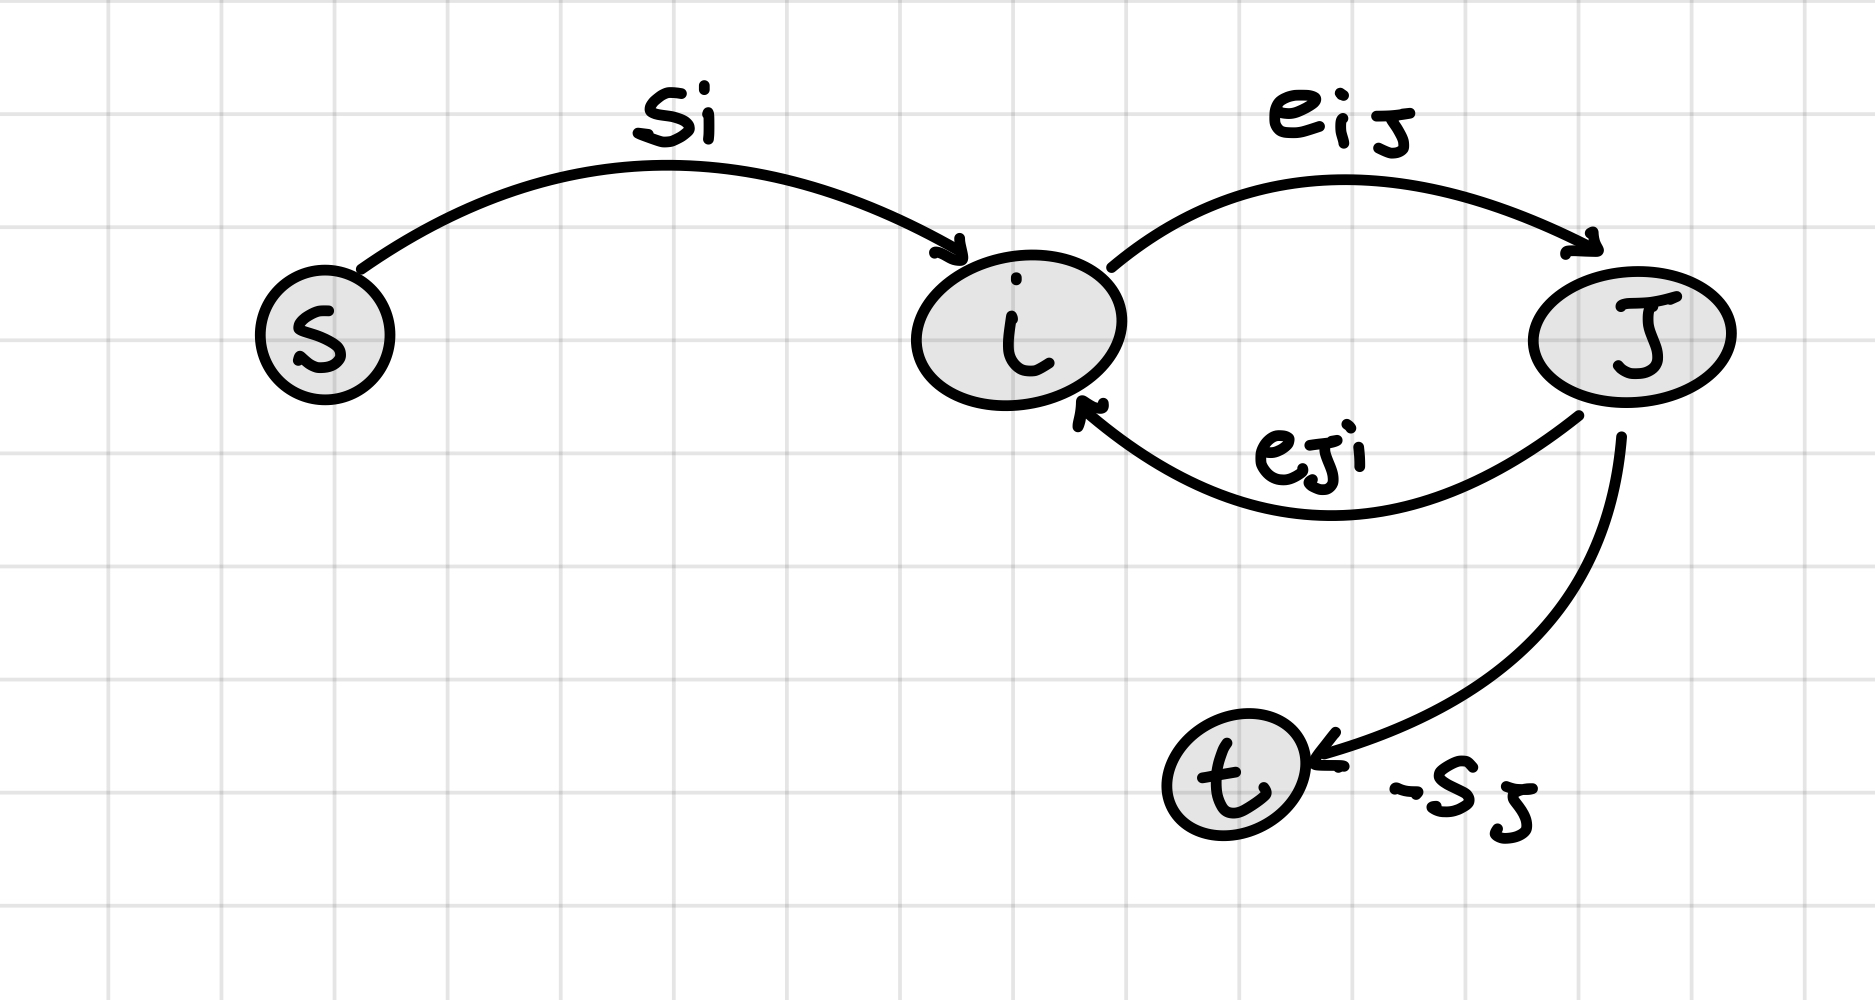
\includegraphics[width=0.5\textwidth]{imm/Immagine JPEG-4101-9BE8-E1-0.jpeg}
\end{figure}
\paragraph{Algorithm.}
Fix any country $k$. For each other country $\ell \neq k$, compute the
minimum $s$-$t$ cut in $G'$ with $k$ forced on the source side and $\ell$
forced on the sink side. A nonempty free-standing proper subset exists if
and only if the minimum such cut has capacity less than
$\sum_{i:\, s_i > 0} s_i$.

Alternatively, run $n-1$ min-cut computations (fixing one country on each
side) and check whether any of them corresponds to a free-standing subset.

\paragraph{Correctness.}
Consider any cut $(A, B)$ with $s \in A$ and $t \in B$. Let $S = A
\setminus \{s\}$ be the set of countries on the source side. The capacity
of this cut is:
\[
\mathrm{cap}(A, B)
= \sum_{\substack{i \in S \\ j \in \bar{S}}} e_{ij}
+ \sum_{\substack{i \in S \\ s_i < 0}} (-s_i)
+ \sum_{\substack{j \in \bar{S} \\ s_j > 0}} s_j.
\]
One can verify that $S$ is free-standing if and only if this cut capacity
is at most $\sum_{i:\, s_i > 0} s_i$, which is the capacity of the trivial
cut $({\{s\}}, V' \setminus \{s\})$. Therefore:

\begin{claim}
Minimizing $\mathrm{cap}(A', V \setminus A')$ over all non-trivial cuts
is equivalent to maximizing $c(A)$, where:
\[
\mathrm{cap}(A', V \setminus A') = P + \sum_{\substack{i \in A \\ j \in A}} e_{ij} - \sum_{i \in A} s_i.
\]
In particular, a free-standing subset exists if and only if
\[
\mathrm{cap}(A', V \setminus A') \leq P.
\]
\end{claim}
\chapter{NP and Computational
Intractability}
%=============================================================
\section{Algorithm Design Patterns and Anti-Patterns}
%=============================================================

Some problems can be solved with well-known \textbf{design patterns}:
\begin{itemize}
    \item \textbf{Greedy} -- e.g., interval scheduling in $O(n \log n)$.
    \item \textbf{Divide-and-conquer} -- e.g., FFT in $O(n \log n)$.
    \item \textbf{Dynamic programming} -- e.g., edit distance in $O(n^2)$.
    \item \textbf{Duality} -- e.g., bipartite matching in $O(n^3)$.
    \item \textbf{Reductions}, local search, randomization.
\end{itemize}

Other problems seem to have \textbf{no efficient algorithm}. These are called \textbf{anti-patterns}:
\begin{itemize}
    \item \textbf{NP-completeness} -- an $O(n^k)$ algorithm is very unlikely.
    \item \textbf{PSPACE-completeness} -- even an $O(n^k)$ certifier is unlikely.
    \item \textbf{Undecidability} -- no algorithm exists at all.
\end{itemize}

%=============================================================
\section{Polynomial-Time Reductions (Section 8.1)}
%=============================================================

\subsection{Classifying Problems}

\textbf{Key question:} Which problems can we solve in practice?\\
\begin{figure}[H]
    \centering
    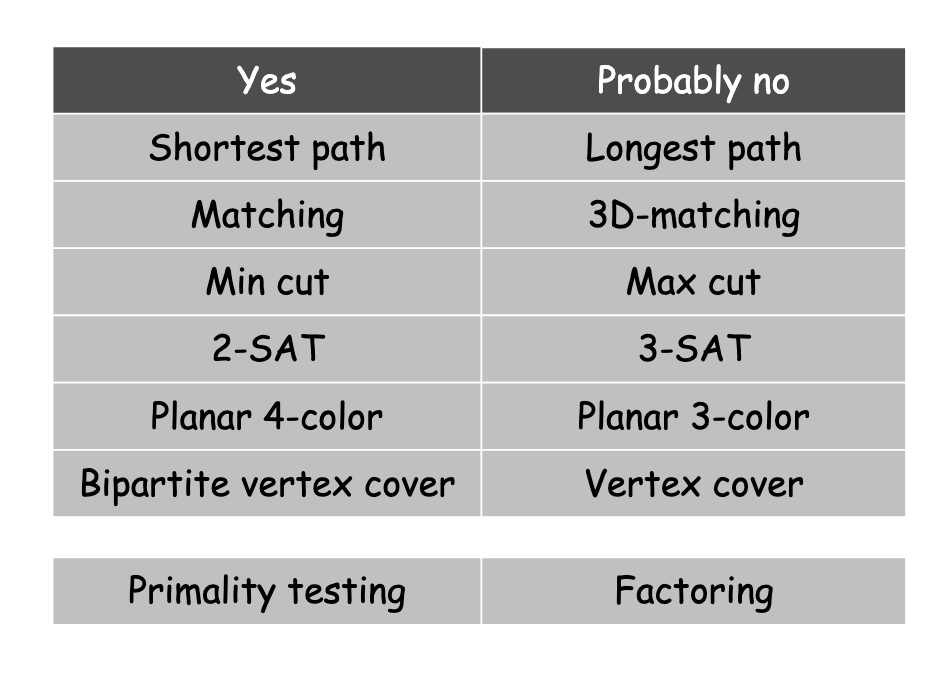
\includegraphics[width=1\textwidth]{imm/Screenshot 2026-05-15 alle 14.30.10.png}
\end{figure}

    
\subsection{Polynomial-Time Reduction}

\begin{definition}{Polynomial-Time Reduction}{}
Problem $X$ \textbf{polynomial reduces} to problem $Y$, written $X \leq_P Y$, if any instance of $X$ can be solved using:
\begin{itemize}
    \item a polynomial number of standard computational steps, plus
    \item a polynomial number of calls to an \textbf{oracle} that solves $Y$.
\end{itemize}
\textbf{Note:} Instances of $Y$ must have polynomial size (we pay to write them down).
\end{definition}

\textbf{Why reductions matter:}
\begin{itemize}
    \item \textbf{Design algorithms:} If $X \leq_P Y$ and $Y$ can be solved in poly-time, then $X$ can too.
    \item \textbf{Prove intractability:} If $X \leq_P Y$ and $X$ has no poly-time algorithm, then $Y$ has no poly-time algorithm either.
    \item \textbf{Prove equivalence:} If $X \leq_P Y$ and $Y \leq_P X$, we write $X \equiv_P Y$.
\end{itemize}

\subsection{Three Basic Reduction Strategies}

\begin{enumerate}
    \item Reduction by \textbf{simple equivalence}.
    \item Reduction from \textbf{special case to general case}.
    \item Reduction by \textbf{encoding with gadgets}.
\end{enumerate}

%--------------------------------------------------------------
\subsection{Strategy 1 --- Simple Equivalence}
%--------------------------------------------------------------

\paragraph{Problem: Independent Set}

\begin{definition}{Independent Set}{}
Given a graph $G = (V, E)$ and an integer $k$: does there exist a subset $S \subseteq V$ with $|S| \geq k$ such that \textbf{no two vertices in $S$ share an edge}?

 \textbf{Independent Set}{}
Consider a graph with 8 nodes.
\end{definition}
\begin{figure}[H]
    \centering
    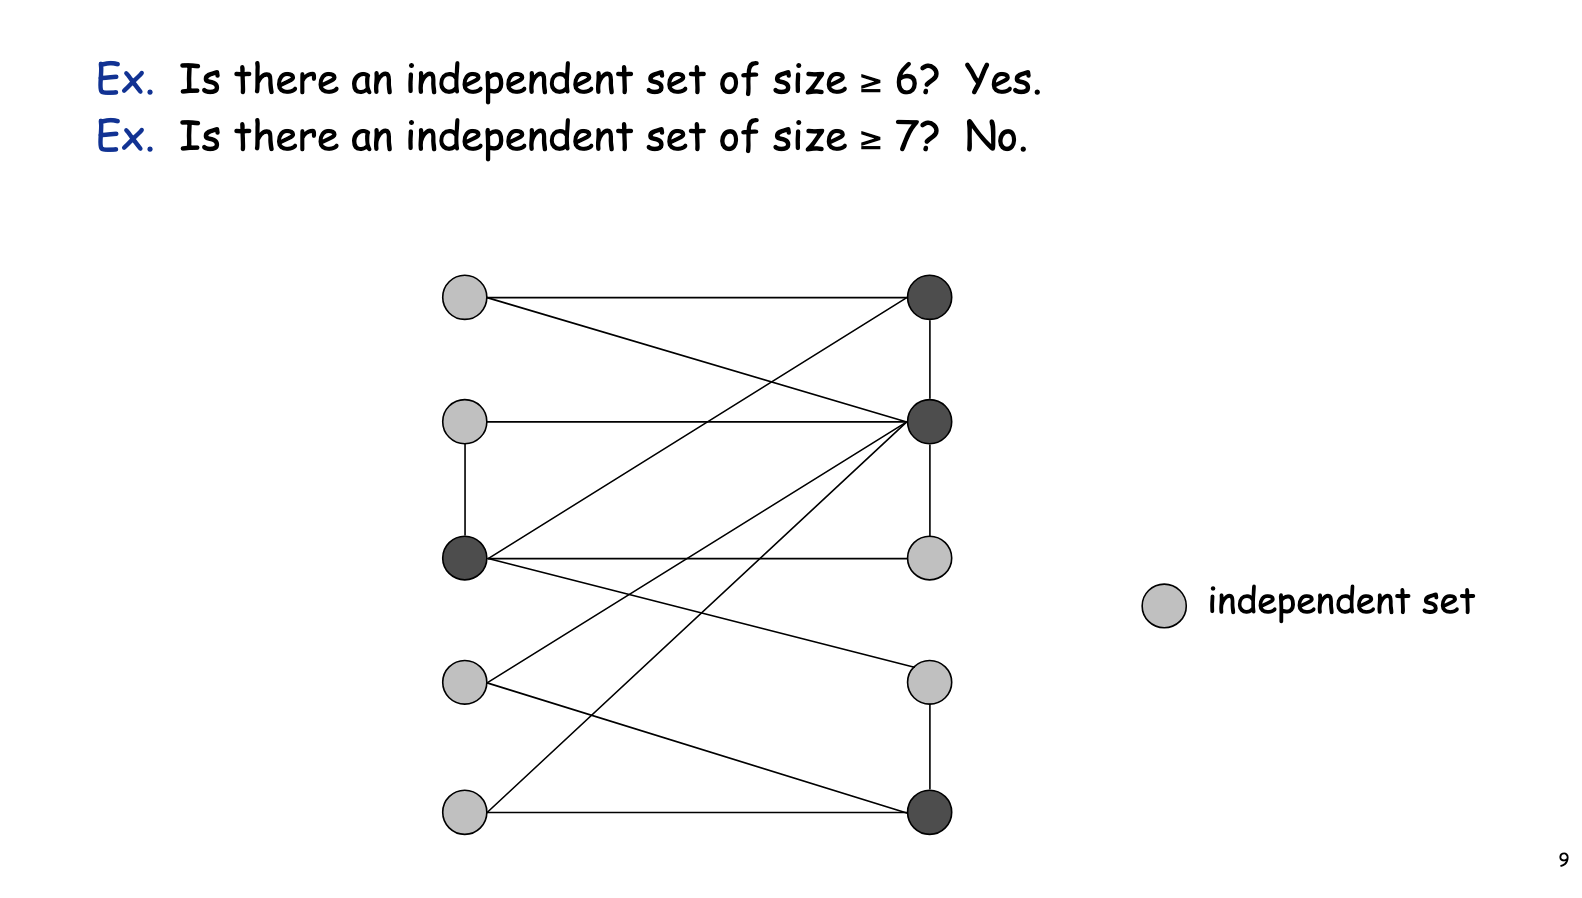
\includegraphics[width=0.5\textwidth]{imm/Screenshot 2026-05-15 alle 14.34.21.png}
\end{figure}
 

\paragraph{Problem: Vertex Cover}

\begin{definition}{Vertex Cover}{}
Given a graph $G = (V, E)$ and an integer $k$: does there exist a subset $S \subseteq V$ with $|S| \leq k$ such that \textbf{every edge has at least one endpoint in $S$}?
\end{definition}

 \textbf{Vertex Cover}{}
On the same graph:
\begin{figure}[H]
    \centering
    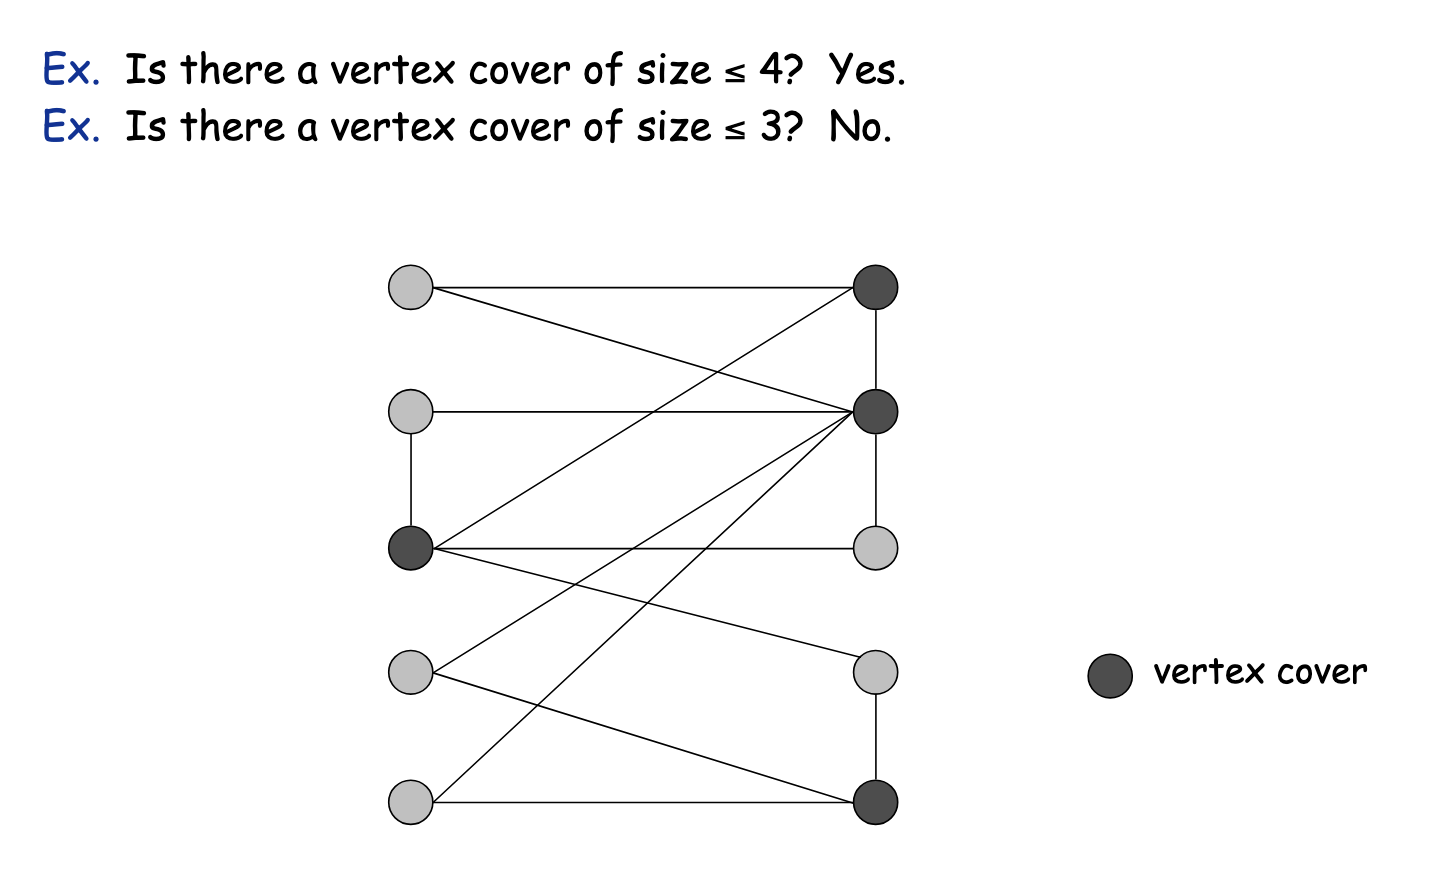
\includegraphics[width=0.5\textwidth]{imm/Screenshot 2026-05-15 alle 14.36.49.png}
\end{figure}
 
min numero di nodi che coprono tutti gli archi
\begin{claim}{VERTEX-COVER $\equiv_P$ INDEPENDENT-SET}{}
$S$ is an independent set $\iff$ $V \setminus S$ is a vertex cover.

\textbf{Proof ($\Rightarrow$):}
Let $S$ be an independent set. Take any edge $(u, v)$.
Since $S$ is independent, $u \notin S$ or $v \notin S$, so $u \in V \setminus S$ or $v \in V \setminus S$.
Thus $V \setminus S$ covers every edge.

\textbf{Proof ($\Leftarrow$):}
Let $V \setminus S$ be a vertex cover. Take any two nodes $u, v \in S$.
The edge $(u, v)$ cannot exist because $V \setminus S$ would need to cover it, but neither $u$ nor $v$ is in $V \setminus S$.
So no two nodes in $S$ are connected $\Rightarrow$ $S$ is independent. $\square$
\end{claim}

%--------------------------------------------------------------
\subsection{Strategy 2 --- Special Case to General Case}
%--------------------------------------------------------------

\begin{definition}{Set Cover}{}
Given a universe $U$ of elements, a collection of subsets $S_1, S_2, \ldots, S_m \subseteq U$, and an integer $k$: does there exist a collection of $\leq k$ sets whose \textbf{union equals $U$}?
\end{definition}

 \textbf{Set Cover}{}
\[
U = \{1, 2, 3, 4, 5, 6, 7\}, \quad k = 2
\]
\[
S_1 = \{3,7\},\quad S_2 = \{3,4,5,6\},\quad S_3 = \{1\},\quad S_4 = \{2,4\},\quad S_5 = \{5\},\quad S_6 = \{1,2,6,7\}
\]
Answer: \textbf{Yes}, choose $S_2$ and $S_6$: their union is $\{1,2,3,4,5,6,7\} = U$.

\textbf{Real-world application:} You have $m$ software packages. Each gives a set $S_i$ of capabilities. Can you cover all $n$ required capabilities using $\leq k$ packages?
 

\begin{claim}{VERTEX-COVER $\leq_P$ SET-COVER}{}
\textbf{Construction:} Given a VERTEX-COVER instance $\langle G=(V,E),\, k \rangle$, create a SET-COVER instance:
\[
k' = k, \quad U = E, \quad S_v = \{e \in E : e \text{ is incident to vertex } v\}
\]
\textbf{Why it works:} A set of vertices covers all edges iff the corresponding sets cover all elements.
A vertex cover of size $\leq k$ exists $\iff$ a set cover of size $\leq k$ exists.

\textbf{Example:} A graph with vertices $\{a,b,c,d,e,f\}$ and edges $\{e_1,\ldots,e_7\}$.\\
Taking $k=2$, vertex cover $\{b,e\}$ corresponds to sets $S_b = \{e_1,e_2,e_3,e_4\}$, $S_e = \{e_4,e_5,e_6,e_7\}$.
\end{claim}
\begin{figure}[H]
    \centering
    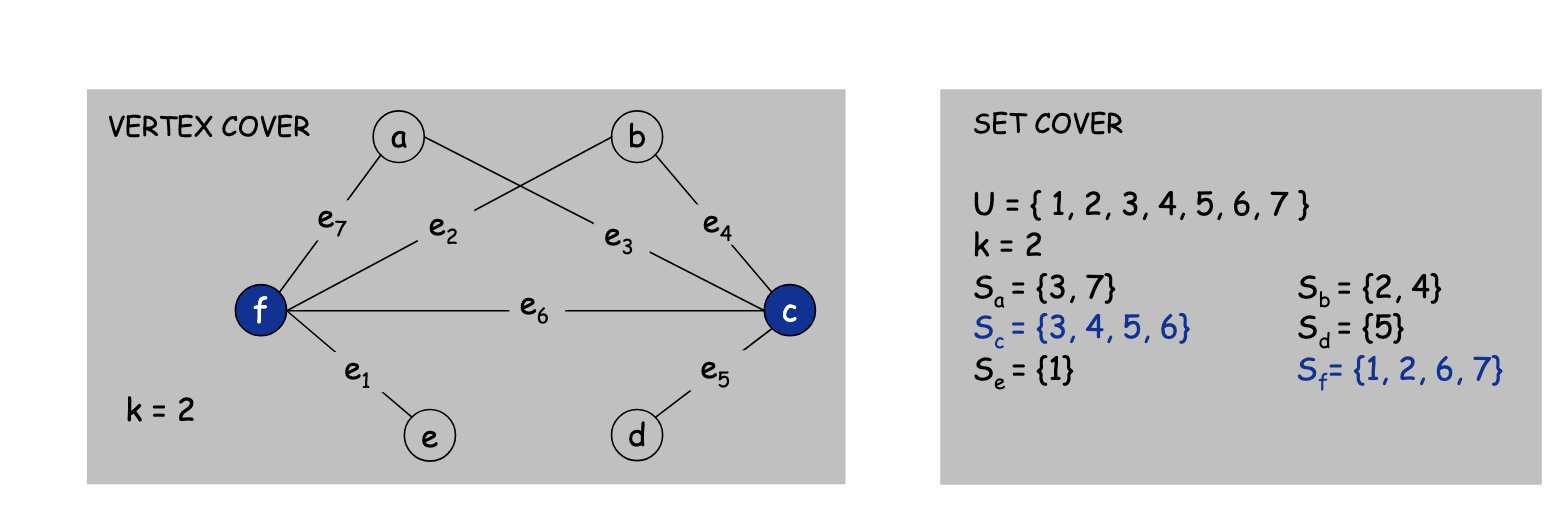
\includegraphics[width=0.5\textwidth]{imm/Screenshot 2026-05-15 alle 16.51.19.png}
\end{figure}

%--------------------------------------------------------------
\subsubsection{Strategy 3 --- Encoding with Gadgets}
%--------------------------------------------------------------

\begin{definition}{SAT and 3-SAT}{}
\begin{itemize}
    \item A \textbf{literal} is a Boolean variable $x_i$ or its negation $\overline{x_i}$.
    \item A \textbf{clause} is a disjunction (OR) of literals: $C_j = x_1 \vee \overline{x_2} \vee x_3$.
    \item A formula in \textbf{Conjunctive Normal Form (CNF)} is a conjunction (AND) of clauses:
    \[
    \Phi = C_1 \wedge C_2 \wedge C_3 \wedge C_4
    \]
    \item \textbf{SAT:} Given a CNF formula $\Phi$, does it have a satisfying truth assignment?
    \item \textbf{3-SAT:} SAT where every clause has \textbf{exactly 3 literals}.
\end{itemize}
\end{definition}

 \textbf{3-SAT}{}
\begin{figure}[H]
    \centering
    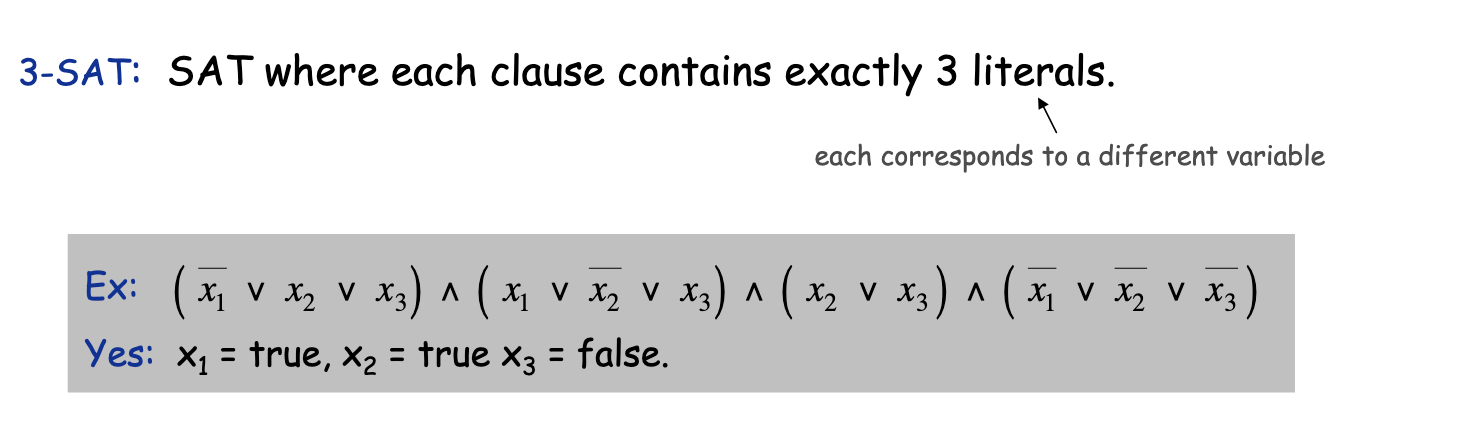
\includegraphics[width=0.7\textwidth]{imm/Screenshot 2026-05-15 alle 16.58.46.png}
\end{figure}

\begin{claim}{3-SAT $\leq_P$ INDEPENDENT-SET}{}
\textbf{Construction:} Given a 3-SAT instance $\Phi$ with $k$ clauses, build graph $G$:
\begin{enumerate}
    \item For each clause, create \textbf{3 vertices} (one per literal). Connect them in a \textbf{triangle}.
    \item Connect each literal vertex to every vertex representing its \textbf{negation} in other clauses.
\end{enumerate}

\textbf{Example:}
\[
\Phi = (x_1 \vee x_2 \vee x_3) \wedge (\overline{x_1} \vee \overline{x_2} \vee x_3) \wedge (x_1 \vee x_2 \vee x_4)
\]
$k = 3$, so we need an independent set of size 3.\\
The graph $G$ has $3 \times 3 = 9$ vertices.\\
Triangle edges (within each clause) + conflict edges (e.g., $x_1$ in clause 1 is connected to $\overline{x_1}$ in clause 2).
\begin{figure}[H]
    \centering
    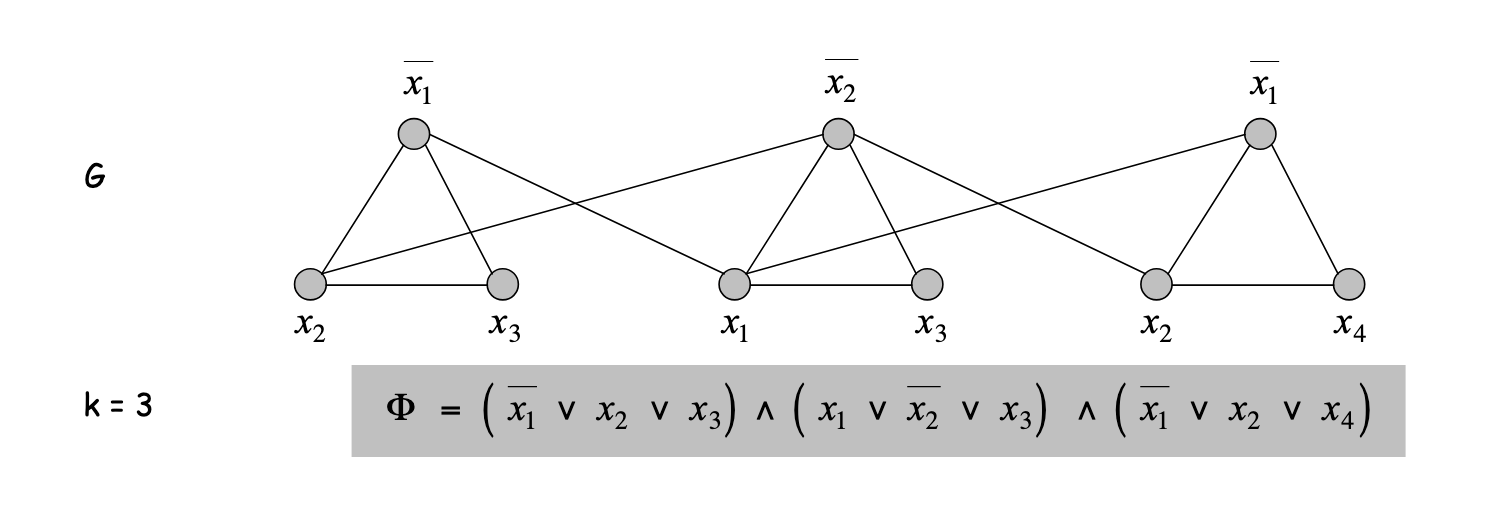
\includegraphics[width=0.7\textwidth]{imm/Screenshot 2026-05-15 alle 17.01.26.png}
\end{figure}
scegliamo questo tipo di scostruzione perchè vogliamo un independent set di dimensione $k$, quindi se ogni clausola è rappresentata da un triangolo, sono costretta a scegliere un vertice quindi un literal per ogni clausola. Inoltre, i conflict edges mi impediscono di scegliere due literal che si contraddicono (es. $x_1$ e $\overline{x_1}$).
\newline
\textbf{Proof:} $G$ has an independent set of size $k$ $\iff$ $\Phi$ is satisfiable.
\begin{itemize}
    \item ($\Rightarrow$) An independent set of size $k$ picks exactly one vertex per triangle (one per clause). Triangles prevent choosing two from the same clause. Conflict edges prevent contradictory assignments. Setting those literals to \texttt{true} satisfies every clause consistently.
    \item ($\Leftarrow$) Given a satisfying assignment, pick one \texttt{true} literal per clause. These form an independent set of size $k$ (no two are in the same triangle, and no two conflict).
\end{itemize}
\end{claim}
in questo caso il set=x3, x1, x4 è un independent set di dimensione 3, quindi $\Phi$ è soddisfacibile (es. $x_1 = x_2 = x_3 = \texttt{true}$, $x_4$ arbitrary).

\subsection{Transitivity of Reductions}

\begin{theorem}{Transitivity}{}
If $X \leq_P Y$ and $Y \leq_P Z$, then $X \leq_P Z$.
\end{theorem}

This means we can \textbf{chain} reductions. A key example:
\[
\text{3-SAT} \leq_P \text{INDEPENDENT-SET} \leq_P \text{VERTEX-COVER} \leq_P \text{SET-COVER}
\]

%=============================================================
\section{Definition of NP (Section 8.3)}
%=============================================================

\subsection{Decision Problems}

A \textbf{decision problem} $X$ is a set of strings. An algorithm $A$ \textbf{solves} $X$ if $A(s) = \texttt{yes} \iff s \in X$.

\textbf{Polynomial time:} $A$ runs in poly-time if for every input $s$, $A(s)$ terminates in at most $p(|s|)$ steps, where $p$ is a polynomial and $|s|$ is the length of $s$.

\subsection{The Class P}

\begin{definition}{Class }
$\mathbf{P}$ is the set of all decision problems solvable by a \textbf{polynomial-time algorithm}.
\end{definition}

 \textbf{Problems in P}{}
\begin{center}
\begin{tabular}{lll}
\toprule
Problem & Question & Algorithm \\
\midrule
MULTIPLE & Is $x$ a multiple of $y$? & Grade school division \\
RELPRIME & Are $x$ and $y$ relatively prime? & Euclid's algorithm \\
PRIMES & Is $x$ prime? & AKS algorithm  \\
EDIT-DISTANCE & Is the edit distance between $x$ and $y$ less than 5? & Dynamic programming \\
LSOLVE & Does $Ax = b$ have a solution? & Gauss-Edmonds elimination \\
\bottomrule
\end{tabular}
\end{center}

\textbf{PRIMES example:}
\begin{itemize}
    \item Input: $s = 53$ (binary string of length $|s| = 6$ bits).
    \item Output: \texttt{yes}, 53 is prime.
    \item Time: $O(|s|^8)$ -- polynomial in the \textbf{length} of the input, not its value.
\end{itemize}
 

\subsection{The Class NP}

\textbf{Intuition:} Instead of \textit{finding} a solution, can we \textit{verify} one quickly?

\begin{definition}{Certifier}{}
Algorithm $C(s, t)$ is a \textbf{certifier} for problem $X$ if for every string $s$:
\[
s \in X \iff \exists\, t \text{ such that } C(s,t) = \texttt{yes}
\]
The string $t$ is called the \textbf{certificate} (or \textit{witness}).
\end{definition}

\begin{definition}{Class}
$\mathbf{NP}$ is the set of decision problems for which there exists a \textbf{poly-time certifier} $C(s,t)$ with $|t| \leq p(|s|)$ for some polynomial $p$.\\
NP stands for \textit{Nondeterministic Polynomial-time}.
\end{definition}

 \textbf{COMPOSITES is in NP}{}
\textbf{Problem:} Given an integer $s$, is $s$ composite (not prime)?\\
\textbf{Certificate:} A nontrivial factor $t$ of $s$ (i.e., $1 < t < s$ and $t \mid s$).\\
\textbf{Certifier:}
\begin{verbatim}
boolean C(s, t) {
    if (t <= 1 or t >= s)  return false;
    if (s mod t == 0)      return true;
    else                   return false;
}
\end{verbatim}
\textbf{Concrete instance:}
\begin{itemize}
    \item $s = 437{,}669$ \quad (Is it composite?)
    \item Certificate: $t = 541$ (or $t = 809$).
    \item Verify: $437{,}669 = 541 \times 809$. \checkmark
    \item Conclusion: \textbf{COMPOSITES is in NP}.
\end{itemize}
\textbf{Why $|t| \leq |s|$?} Any factor of $s$ is at most $s$, so it has at most the same number of bits.
 

 \textbf{SAT is in NP}{}
\textbf{Problem:} Given a CNF formula $\Phi$, does it have a satisfying assignment?\\
\textbf{Certificate:} An assignment of truth values to all $n$ Boolean variables.\\
\textbf{Certifier:} Check that each clause contains at least one \texttt{true} literal.\\
\textbf{Concrete instance:}
\[
\Phi = (x_1 \vee \overline{x_2} \vee \overline{x_3}) \wedge (\overline{x_1} \vee x_2 \vee \overline{x_3}) \wedge (\overline{x_1} \vee \overline{x_2} \vee x_4) \wedge (x_1 \vee \overline{x_3} \vee \overline{x_4})
\]
Certificate: $x_1 = 1,\, x_2 = 1,\, x_3 = 0,\, x_4 = 1$.\\
Check clause 1: $1 \vee 0 \vee 1 = 1$. $\checkmark$\quad Check clause 2: $0 \vee 1 \vee 1 = 1$. $\checkmark$\quad (all clauses satisfied)\\
\textbf{Conclusion: SAT is in NP}.
 

 \textbf{HAM-CYCLE is in NP}{}
\textbf{Problem:} Given an undirected graph $G=(V,E)$, does there exist a \textbf{Hamiltonian cycle} -- a simple cycle that visits every node exactly once?\\
\textbf{Certificate:} A permutation of all $n$ nodes.\\
\textbf{Certifier:}
\begin{enumerate}
    \item Check that the permutation contains each node in $V$ exactly once.
    \item Check that there is an edge between each pair of adjacent nodes in the permutation.
    \item Check that there is an edge between the last and first node (to close the cycle).
\end{enumerate}
\begin{figure}[H]
    \centering
    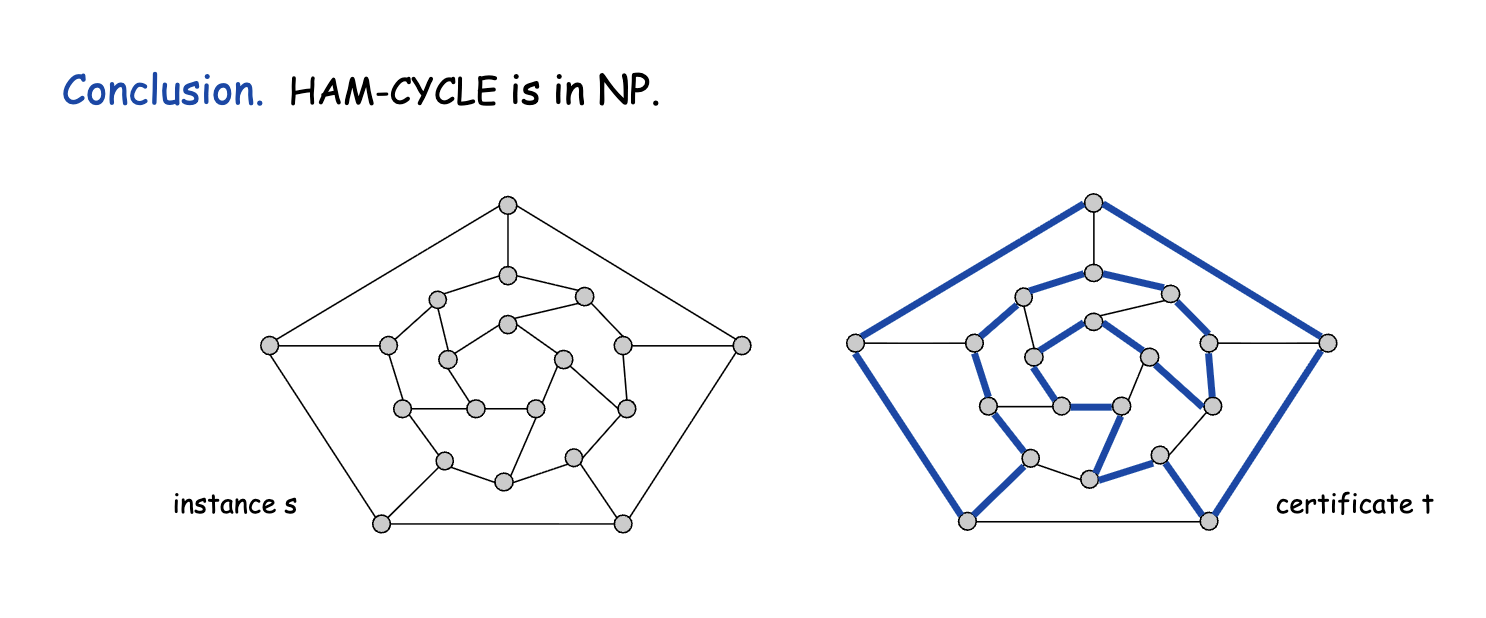
\includegraphics[width=0.5\textwidth]{imm/Screenshot 2026-05-15 alle 19.10.50.png}
\end{figure}
\textbf{Conclusion: HAM-CYCLE is in NP}. (The certifier runs in $O(n)$ -- polynomial.)
 

\subsection{P, NP, and EXP}

\begin{definition}{Class }
$\mathbf{EXP}$ is the set of decision problems solvable by an \textbf{exponential-time} algorithm.
\end{definition}

\begin{theorem}{Inclusion Chain}{}
\[
P \subseteq NP \subseteq EXP
\]
\textbf{Proof of $P \subseteq NP$:} If algorithm $A(s)$ solves $X$ in poly-time, use empty certificate $\varepsilon$ and define $C(s, \varepsilon) = A(s)$. So $X \in NP$.

\textbf{Proof of $NP \subseteq EXP$:} For $X \in NP$, there exists a poly-time certifier $C(s,t)$.\\
To solve input $s$: run $C(s,t)$ on all strings $t$ with $|t| \leq p(|s|)$.\\
There are at most $2^{p(|s|)}$ such strings -- exponentially many, but finite.\\
Return \texttt{yes} if any call returns \texttt{yes}. This is an exponential algorithm. $\square$
\end{theorem}

\subsection{The P vs. NP Question}

\textbf{The biggest open question in computer science:} Does $P = NP$?

\begin{itemize}
    \item If \textbf{$P = NP$}: efficient algorithms exist for 3-SAT, TSP, 3-COLOR, FACTOR, \ldots\\ This would \textbf{break RSA cryptography} and potentially collapse the economy.
    \item If \textbf{$P \neq NP$}: no efficient algorithm exists for NP-complete problems.
    \item \textbf{Consensus:} most researchers believe $P \neq NP$. (Probably no.)
 
\end{itemize}

\begin{center}
\begin{tabular}{cc}
\toprule
\textbf{If $P \neq NP$} & \textbf{If $P = NP$} \\
\midrule
$EXP \supset NP \supset P$ & $EXP \supset P = NP$ \\
(all three classes are distinct) & (P and NP collapse together) \\
\bottomrule
\end{tabular}
\end{center}

%=============================================================
\section{NP-Completeness (Section 8.4)}
%=============================================================

\subsection{Two Types of Reduction}

\begin{itemize}
    \item \textbf{Cook reduction ($\leq_P$):} solve $X$ using a polynomial number of oracle calls to $Y$.
    \item \textbf{Karp transformation:} given input $x$ to $X$, construct $y$ (in poly-time) such that $x \in X \iff y \in Y$. (Only \textbf{one oracle call}, at the very end.)
\end{itemize}

Almost all reductions seen in practice are \textbf{Karp transformations}. The open question is whether these two definitions are actually equivalent.

\subsection{NP-Complete Problems}

\begin{definition}{NP-Complete}{}
A problem $Y$ is \textbf{NP-complete} if:
\begin{enumerate}
    \item $Y \in NP$.
    \item For every $X \in NP$: $X \leq_P Y$.
    \quad (``$Y$ può risolvere qualsiasi problema in NP''.)
\end{enumerate}
\end{definition}

\begin{theorem}{Central Theorem}{}
Suppose $Y$ is NP-complete. Then $Y$ is solvable in poly-time $\iff$ $P = NP$.

\textbf{Proof ($\Leftarrow$):} If $P = NP$, then since $Y \in NP$, $Y \in P$, so $Y$ is solvable in poly-time.

\textbf{Proof ($\Rightarrow$):} Suppose $Y$ is solvable in poly-time. Let $X$ be any problem in NP.\\
Since $X \leq_P Y$, we can solve $X$ in poly-time $\Rightarrow NP \subseteq P$.\\
We already know $P \subseteq NP$, so $P = NP$. $\square$
\end{theorem}

\subsection{Circuit Satisfiability --- The First NP-Complete Problem}

\begin{definition}{CIRCUIT-SAT}{}
Given a combinational circuit built from AND, OR, and NOT gates, where some inputs are \textbf{fixed} (hard-coded 0 or 1) and some are \textbf{free} (the inputs we can choose): can we set the free inputs so the circuit \textbf{output is 1}?
\end{definition}
\begin{figure}[H]
\centering
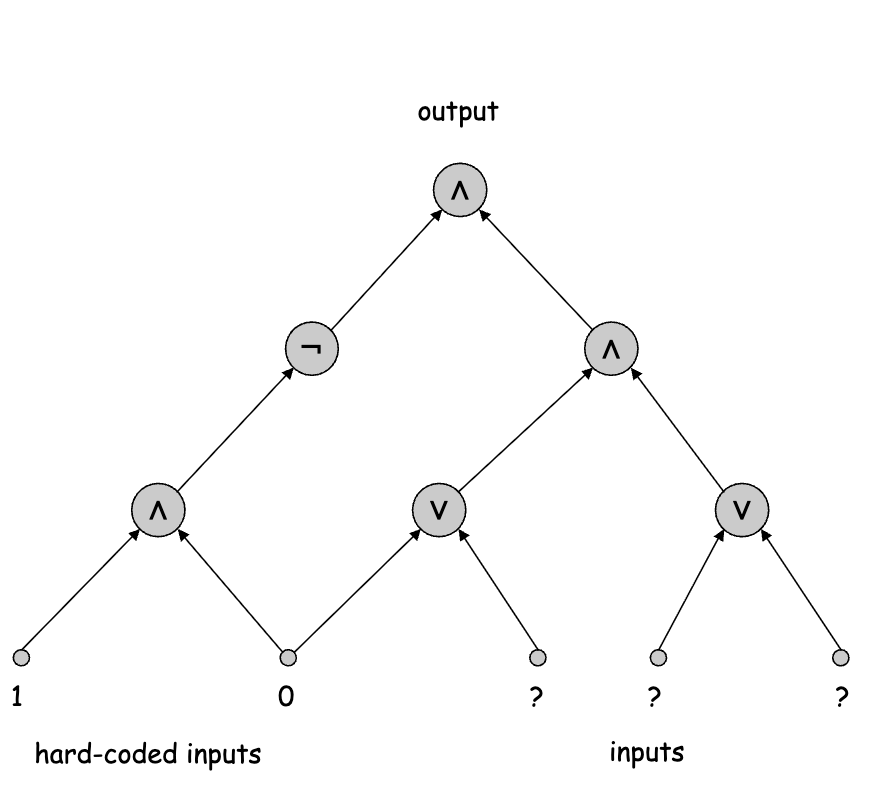
\includegraphics[width=0.4\textwidth]{imm/Screenshot 2026-05-15 alle 13.45.57.png}
\end{figure}

\textbf{Question:} Can we set $x_2, x_3, x_4 \in \{0,1\}$ so the output is 1?\\
\textbf{Example answer:} $x_2=1, x_3=0, x_4=1$ produces output 1. $\checkmark$
 

\begin{theorem}{Cook-Levin Theorem (1971/1973)}{}
\textbf{CIRCUIT-SAT is NP-complete.}

\textbf{Proof sketch:}
\begin{itemize}
    \item \textit{CIRCUIT-SAT $\in$ NP:} Certificate = a setting of the free inputs. Certifier = simulate the circuit ($O(n)$ time).
    \item \textit{Every NP problem $\leq_P$ CIRCUIT-SAT:} For any $X \in NP$ with certifier $C(s,t)$:
    \begin{enumerate}
        \item View $C(s,t)$ as an algorithm on $|s| + p(|s|)$ input bits (fixed $s$, free $t$).
        \item Since $C$ runs in poly-time, it can be converted into a poly-size circuit $K$.
        \item Hard-code the first $|s|$ bits with the input $s$.
        \item The remaining $p(|s|)$ bits represent the certificate $t$ (free inputs).
        \item $K$ is satisfiable $\iff$ $C(s,t) = \texttt{yes}$ for some $t$ $\iff$ $s \in X$.
    \end{enumerate}
\end{itemize}

\textbf{Concrete example:} Encode the INDEPENDENT-SET certifier as a circuit.\\
For graph $G = (V,E)$ with $n=3$ (nodes $u,v,w$) and $k=2$:
\begin{figure}[H]
\centering
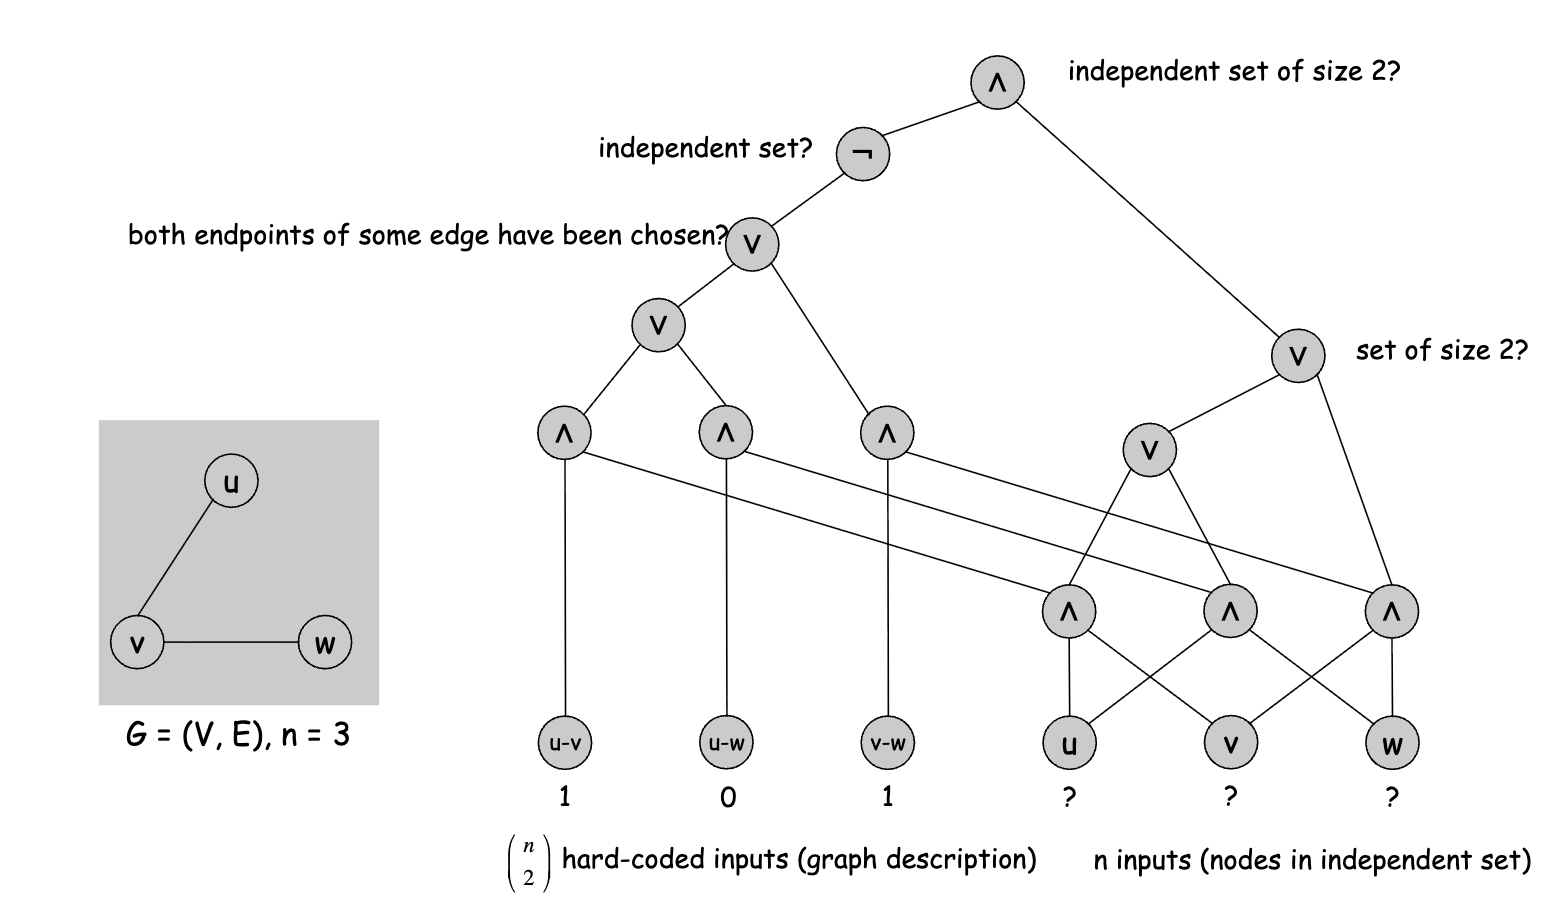
\includegraphics[width=0.6\textwidth]{imm/Screenshot 2026-05-15 alle 13.54.54.png}
\end{figure}


\begin{itemize}
    \item The circuit has $n=3$ free inputs (which nodes to include).
    \item Hard-coded inputs encode the graph structure (which edges exist).
    \item The circuit outputs 1 iff the chosen nodes form an independent set of size 2.
\end{itemize}
\end{theorem}

\subsection{Recipe to Prove NP-Completeness}

Once CIRCUIT-SAT is established, \textbf{other NP-complete problems fall like dominoes.}

    \begin{enumerate}
    \item \textbf{Show $Y \in NP$:} Describe a certificate and a poly-time certifier.
    \item \textbf{Choose a known NP-complete problem $X$} (e.g., CIRCUIT-SAT, 3-SAT).
    \item \textbf{Prove $X \leq_P Y$:} Construct a poly-time transformation.
\end{enumerate}
\textbf{Justification:} If $W \in NP$, then $W \leq_P X \leq_P Y$ (by transitivity), so $Y$ is NP-complete.


\subsection{3-SAT is NP-Complete}

\begin{theorem}{3-SAT is NP-complete}{}
\textbf{Proof:} 3-SAT $\in$ NP (certificate: truth assignment). It suffices to show CIRCUIT-SAT $\leq_P$ 3-SAT.

\textbf{Construction:} Given a circuit $K$, create a 3-SAT variable $x_i$ for each element (gate or wire) $i$. Add clauses to force correct computation:

\begin{center}
\begin{tabular}{lll}
\toprule
\textbf{Gate type} & \textbf{Constraint} & \textbf{Clauses added} \\
\midrule
NOT gate & $x_2 = \neg x_3$ & $(\overline{x_2} \vee \overline{x_3}) \wedge (x_2 \vee x_3)$ \quad (2 clauses) \\
OR gate & $x_1 = x_4 \vee x_5$ & 3 clauses \\
AND gate & $x_0 = x_1 \wedge x_2$ & 3 clauses \\
Hard-coded 0 & $x_5 = 0$ & $(\overline{x_5})$ \quad (1 clause) \\
Output = 1 & $x_0 = 1$ & $(x_0)$ \quad (1 clause) \\
\bottomrule
\end{tabular}
\end{center}

Short clauses (of length 1 or 2) are padded to length exactly 3 using new dummy variables.\\
\textbf{Result:} The formula is satisfiable $\iff$ the circuit is satisfiable. $\square$
\end{theorem}

\subsection{The Domino Chain of NP-Complete Problems}

All problems below are NP-complete and reduce to one another:
\[
\text{CIRCUIT-SAT} \leq_P \text{3-SAT} \leq_P \text{INDEPENDENT-SET} \leq_P \text{VERTEX-COVER} \leq_P \text{SET-COVER}
\]
Also NP-complete: DIR-HAM-CYCLE, HAM-CYCLE, TSP, GRAPH 3-COLOR, SUBSET-SUM, SCHEDULING, PLANAR 3-COLOR, \ldots

\begin{figure}[H]
\centering
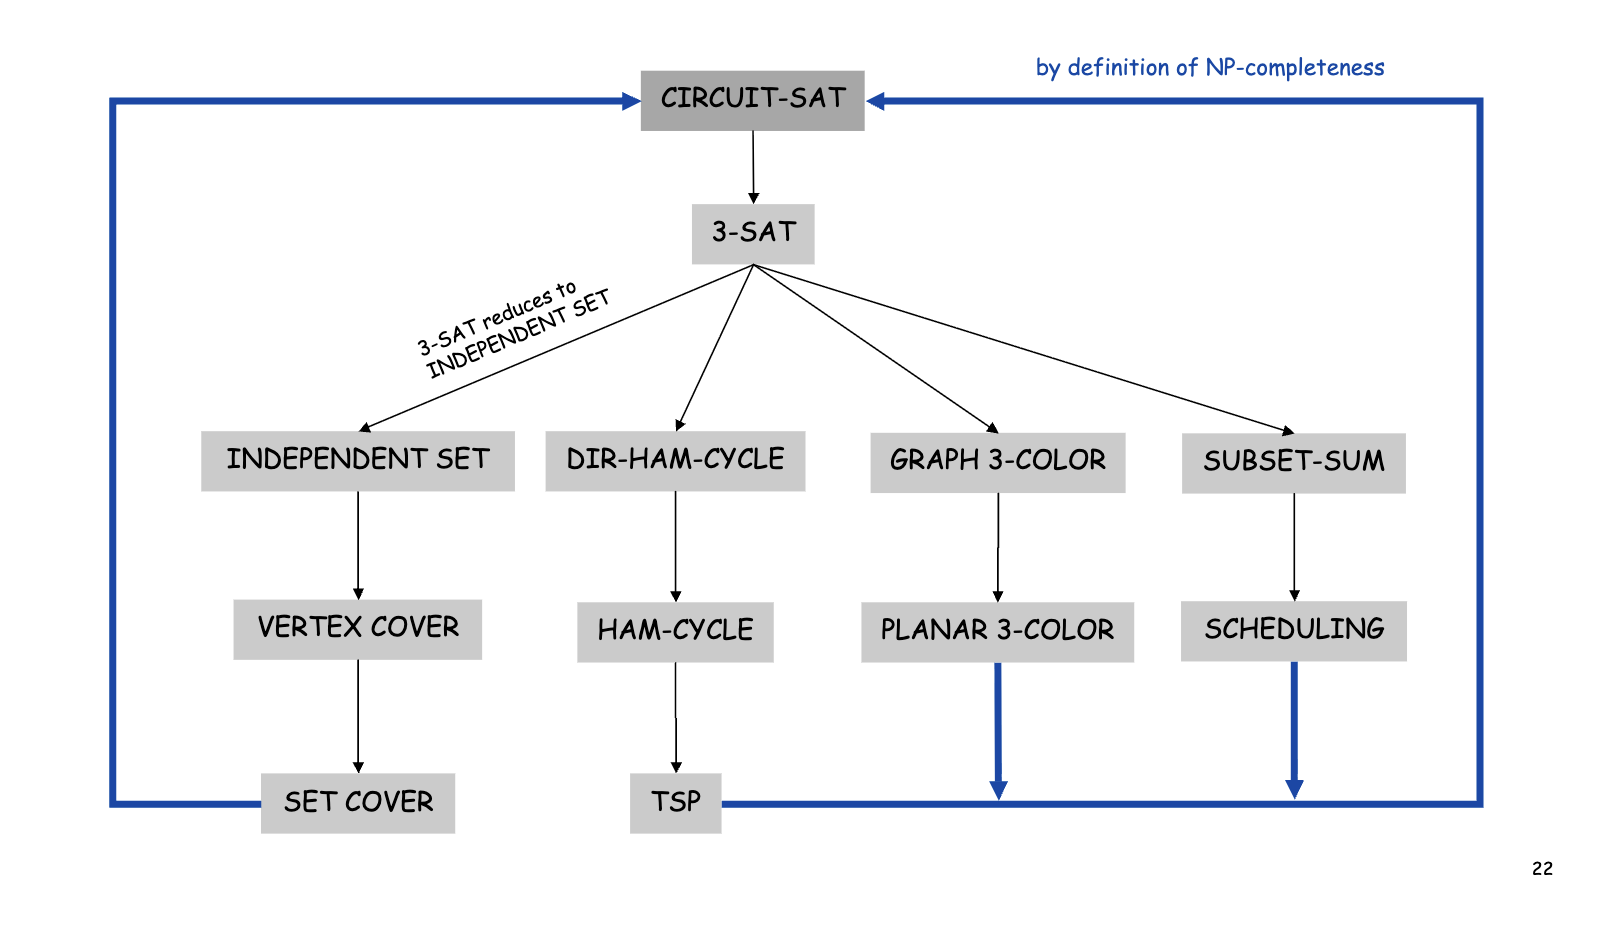
\includegraphics[width=0.8\textwidth]{imm/Screenshot 2026-05-15 alle 14.21.14.png}
\end{figure}


Most NP problems are either known to be in $P$ or NP-complete. Notable exceptions (in between, not known to be either): FACTORING, graph isomorphism, Nash equilibrium.


MANCAAAAA
\section{Sequencing Problems (Section 8.5)}
%=============================================================

\subsection{Hamiltonian Cycle}
\textbf{HAM-CYCLE:} Given an undirected graph $G$, does there exist a simple cycle that contains every node in $V$?

\textbf{DIR-HAM-CYCLE:} Given a directed graph $G$, does there exist a simple directed cycle that contains every node in $V$?

\begin{theorem}{DIR-HAM-CYCLE reduces to HAM-CYCLE}{}
DIR-HAM-CYCLE $\leq_P$ HAM-CYCLE.
\end{theorem}
\textbf{Proof:} We transform a directed graph $G$ into an undirected graph $G'$. For each node $v$ in $G$, we create 3 nodes in $G'$: $v_{in}$, $v$, and $v_{out}$, connected in a line. We connect directed edges $(u, v)$ as undirected edges between $u_{out}$ and $v_{in}$. A Hamiltonian cycle in $G'$ must traverse the nodes as $v_{in} \to v \to v_{out}$, perfectly mimicking a directed cycle in $G$.

\begin{theorem}{3-SAT reduces to DIR-HAM-CYCLE}{}
3-SAT $\leq_P$ DIR-HAM-CYCLE.
\end{theorem}
\textbf{Proof Sketch:} We construct a graph with $2^n$ Hamiltonian cycles corresponding to $2^n$ truth assignments. We create a "row" of nodes for each variable $x_i$, which can be traversed left-to-right ($x_i = 1$) or right-to-left ($x_i = 0$). For each clause $C_j$, we create a "clause node". We connect the row nodes to the clause node so that the cycle can only detour through the clause node if the variable traverses in the "correct" direction (satisfying the clause).

\subsection{Traveling Salesperson Problem (TSP)}
\textbf{TSP:} Given a set of $n$ cities and distances $d(u,v)$, is there a tour of length $\leq D$?

\begin{theorem}{HAM-CYCLE reduces to TSP}{}
HAM-CYCLE $\leq_P$ TSP.
\end{theorem}
\textbf{Proof:} Given an instance $G$ of HAM-CYCLE, we create $n$ cities. We set the distance $d(u,v) = 1$ if $(u,v)$ is an edge in $G$, and $d(u,v) = 2$ if it is not. A TSP tour of length $\leq n$ exists if and only if all edges used have distance 1, meaning $G$ has a Hamiltonian cycle.

%=============================================================
\section{Partitioning Problems (Section 8.6)}
%=============================================================

\subsection{3-Dimensional Matching}
\textbf{3D-MATCHING:} Given disjoint sets $X, Y, Z$, each of size $n$, and a set of triples $T \subseteq X \times Y \times Z$, is there a set of $n$ triples such that every element is covered exactly once?
\textit{(Example: Matching instructors, courses, and times).}

\begin{theorem}{3-SAT reduces to 3D-MATCHING}{}
3-SAT $\leq_P$ 3D-MATCHING.
\end{theorem}
\textbf{Proof Sketch:} We create "core" and "tip" gadgets for each variable (representing True/False), "clause" gadgets to ensure one literal per clause is satisfied, and "cleanup" gadgets to cover unused tips.

%=============================================================
\section{Graph Coloring (Section 8.7)}
%=============================================================

\subsection{3-Colorability}
\textbf{3-COLOR:} Given an undirected graph $G$, can you color the nodes with 3 colors (Red, Green, Blue) so no adjacent nodes have the same color?
\textit{(Application: Register allocation in compilers).}

\begin{theorem}{3-SAT reduces to 3-COLOR}{}
3-SAT $\leq_P$ 3-COLOR.
\end{theorem}
\textbf{Proof Sketch:} We create a triangle of nodes: True (T), False (F), Base (B). For each literal $x_i$, we connect it to its negation $\neg x_i$ and to the Base. This forces each literal to be colored T or F. For each clause, we add a 6-node gadget connected to the clause's literals and to B and F. This gadget can only be 3-colored if at least one literal is colored True.

%=============================================================
\section{Numerical Problems (Section 8.8)}
%=============================================================

\subsection{Subset Sum}
\textbf{SUBSET-SUM:} Given natural numbers $w_1, \ldots, w_n$ and a target $W$, is there a subset that adds up exactly to $W$?

\begin{theorem}{3-SAT reduces to SUBSET-SUM}{}
3-SAT $\leq_P$ SUBSET-SUM.
\end{theorem}
\textbf{Proof Sketch:} We create integers using base-10 digits. The digits represent variables and clauses. We choose numbers so that getting the exact sum $W$ requires selecting either $x_i$ or $\neg x_i$ (truth assignment) and covering every clause column. We use "dummy" numbers to handle carry-overs in the clause columns.

\subsection{Scheduling With Release Times}
\textbf{SCHEDULE-RELEASE-TIMES:} Can we schedule $n$ jobs, where job $i$ has processing time $t_i$, release time $r_i$, and deadline $d_i$?

\begin{theorem}{SUBSET-SUM reduces to SCHEDULE-RELEASE-TIMES}{}
SUBSET-SUM $\leq_P$ SCHEDULE-RELEASE-TIMES.
\end{theorem}
\textbf{Proof Sketch:} Create jobs with lengths equal to $w_i$. Create one special job 0 with length 1, release $W$, and deadline $W+1$. This forces job 0 to run exactly at time $W$. The other jobs must fill the space exactly up to $W$ and exactly after $W+1$. This perfectly mimics SUBSET-SUM.

\chapter{APPROXIMATION ALGORITHMS(11)}

%=============================================================
\section{Coping with NP-completeness}
%=============================================================

Some problems are NP-hard, which means we believe no polynomial-time algorithm can solve them exactly. So what do we do in practice?

We have to give something up. There are three things we would like an algorithm to have:
\begin{enumerate}
    \item It works on \textbf{any} input (not just easy special cases).
    \item It finds the \textbf{exact best} solution (optimal).
    \item It runs in \textbf{polynomial time} (fast).
\end{enumerate}
Since we cannot have all three for NP-hard problems, we give up on \textbf{point 2}: we accept a solution that is \textit{not perfect}, but is \textit{provably close} to the best possible.

\begin{definition}{$\rho$-Approximation Algorithm}{}
A \textbf{$\rho$-approximation algorithm} is an algorithm that always:
\begin{itemize}
    \item runs in polynomial time,
    \item gives a solution whose cost is at most $\rho$ times the true optimal cost (for minimization problems).
\end{itemize}
If $\rho = 2$, the algorithm is a \textbf{2-approximation}: it always finds a solution at most \textbf{twice as bad} as the best possible.
\end{definition}

\textbf{The key challenge:} To prove the approximation ratio $\rho$, we need to compare our solution to the optimal. But we do not know the optimal! The trick is to use \textbf{lower bounds} --- quantities that the optimal must be at least, even if we cannot compute the optimal directly.

%=============================================================
\section{Load Balancing}
%=============================================================

\subsection{The Problem}

Imagine you have $m$ machines and $n$ jobs. Each job $j$ takes $t_j$ units of time and must run on exactly one machine. You want to split the jobs across machines so that no machine is overloaded.

Formally:
\begin{itemize}
    \item The \textbf{load} of machine $i$ is $L_i = \sum_{j \in J(i)} t_j$ (sum of times of all jobs on machine $i$).
    \item The \textbf{makespan} is $L = \max_i L_i$ (the time when the last machine finishes).
    \item \textbf{Goal:} minimise the makespan.
\end{itemize}
\begin{figure}[H]
    \centering
    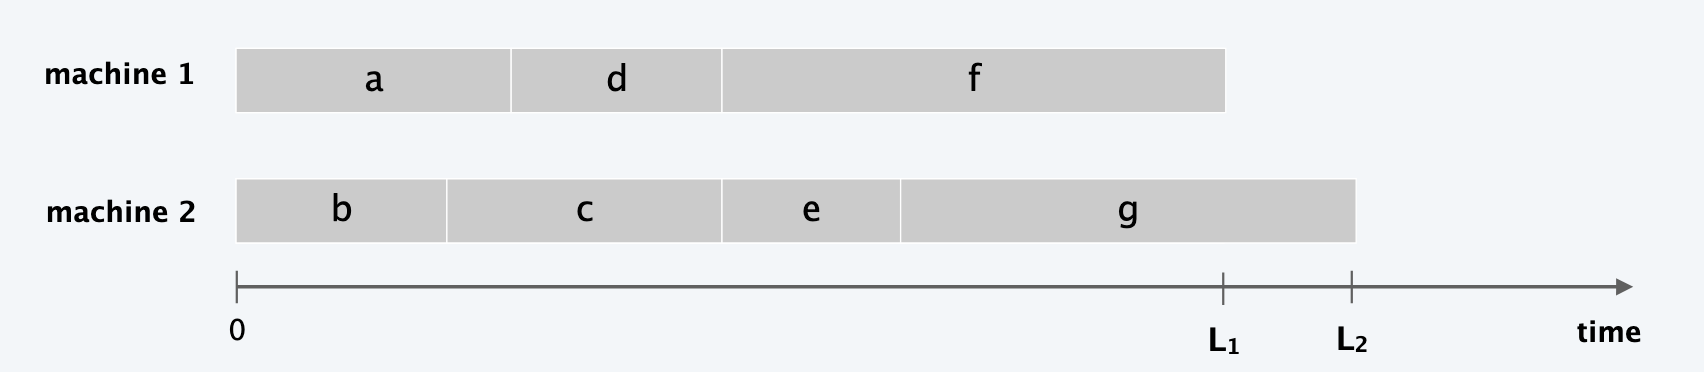
\includegraphics[width=0.5\textwidth]{imm/Screenshot 2026-05-15 alle 17.50.36.png}
\end{figure}

\textit{This problem is NP-hard even with only 2 machines.}
\newline
questo problema è riconducibile al number partitioning problem, che è NP-hard. Se avessimo un algoritmo polinomiale per il load balancing, potremmo usarlo per risolvere il number partitioning: basta mettere i numeri come job e le due partizioni come macchine. Se il load balancing restituisce un makespan di 0, allora i numeri possono essere divisi in due partizioni con somma uguale (soluzione al number partitioning). Se restituisce un makespan maggiore di 0, allora non esiste una partizione perfetta.
\subsection{Algorithm 1: List Scheduling (Greedy)}
\begin{figure}[H]
    \centering
    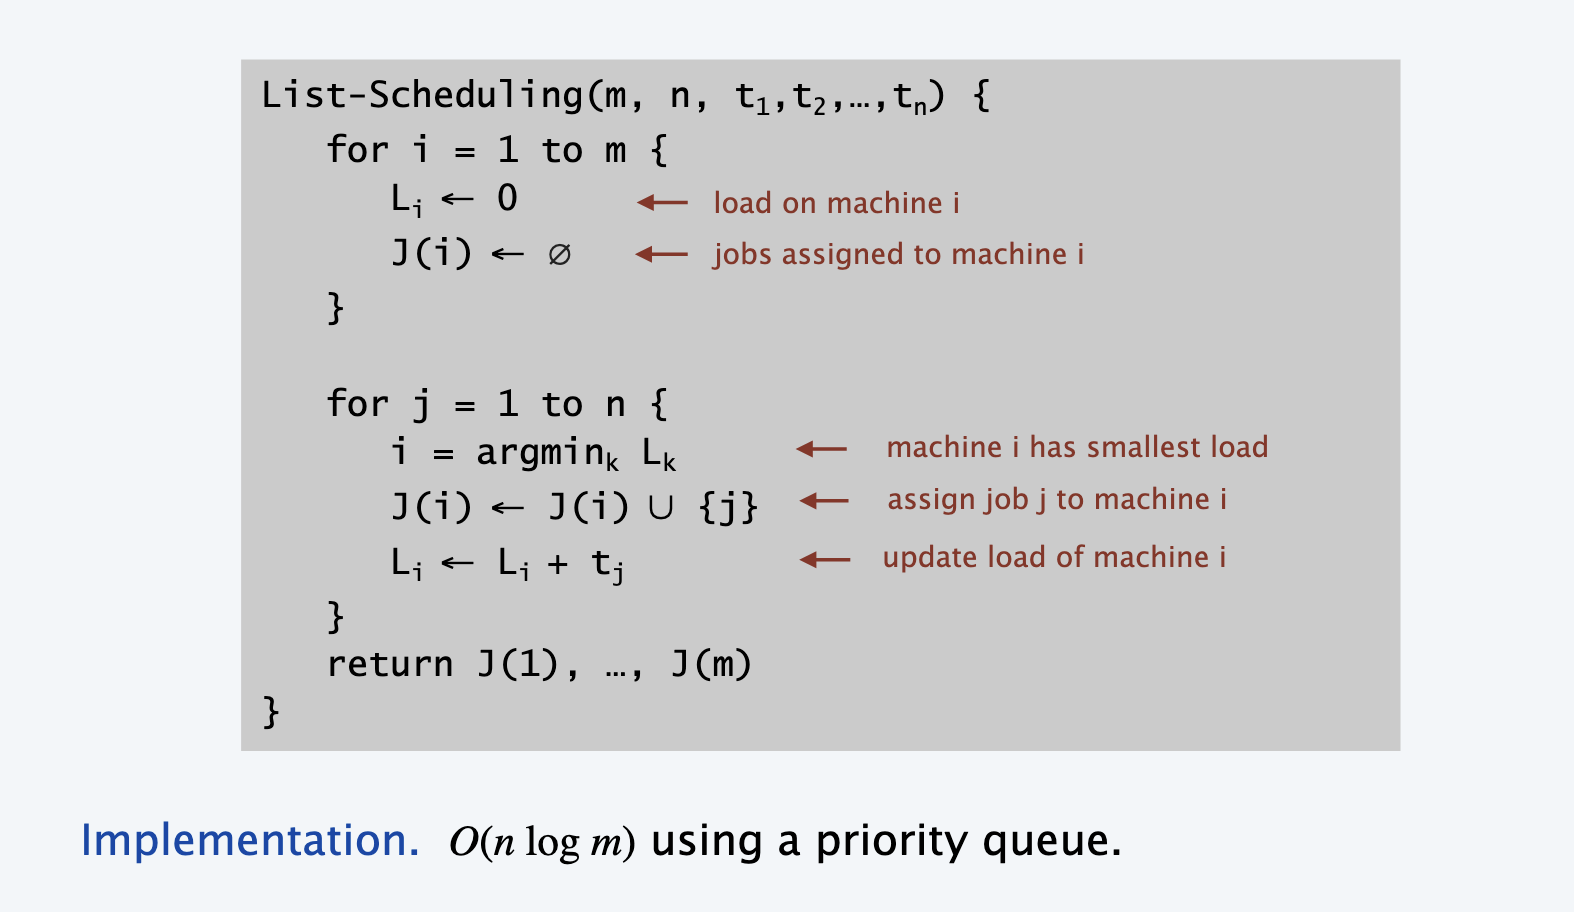
\includegraphics[width=1\textwidth]{imm/Screenshot 2026-05-15 alle 18.04.59.png}
\end{figure}
\textbf{Idea:} Go through the jobs one by one, and always put the next job on the machine that currently has the least work.

\textbf{List Scheduling}{}
3 machines, jobs with times $[3, 3, 2, 2, 10]$.\\
\begin{itemize}
    \item Job 1 ($t=3$) $\to$ Machine 1. Loads: [3, 0, 0].
    \item Job 2 ($t=3$) $\to$ Machine 2 (smallest load). Loads: [3, 3, 0].
    \item Job 3 ($t=2$) $\to$ Machine 3. Loads: [3, 3, 2].
    \item Job 4 ($t=2$) $\to$ Machine 3. Loads: [3, 3, 4].
    \item Job 5 ($t=10$) $\to$ Machine 1 or 2. Loads: [13, 3, 4].
\end{itemize}
Makespan $= 13$. (The optimal is also 10, so this is close but not perfect.)


\subsection{Lower Bounds on the Optimal $L^*$}

We need two facts about the optimal makespan $L^*$ that we can prove without knowing $L^*$ exactly.

\begin{lemma}{Two Lower Bounds}{}
\begin{enumerate}
    \item $L^* \geq \max_j t_j$ \quad (the optimal cannot be less than the longest single job, because some machine must run it).
    \item $L^* \geq \dfrac{1}{m} \sum_j t_j$ \quad (the optimal cannot be less than the average load: the total work is $\sum t_j$, split among $m$ machines, so at least one machine must do at least the average share).
\end{enumerate}
\end{lemma}

\subsection{Analysis: List Scheduling is a 2-Approximation}

\begin{theorem}{List Scheduling $\leq 2 L^*$(l'algoritmo è una 2-approssimazione, cioè trova al massimo una soluzione che è doppia alla soluzione ottima)}


\textbf{Proof (step by step):}
\begin{enumerate}
    \item Let $i$ be the \textbf{bottleneck machine} (the machine with the highest load $L_i = L$).
    \item Let $j$ be the \textbf{last job assigned to machine $i$}.
    \item At the moment job $j$ was assigned, machine $i$ had the \textbf{smallest load} of all machines (that is why the algorithm chose it). So its load at that moment was $L_i - t_j$, and:
    \[
    L_i - t_j \leq L_k \quad \text{for every other machine } k.
    \]
    \item Summing this inequality over all $m$ machines and dividing by $m$:
    \[
    L_i - t_j \leq \frac{1}{m}\sum_{k=1}^m L_k = \frac{1}{m}\sum_j t_j \leq L^* \qquad \text{(by Lemma, part 2 )} \]
    \[ \text{Se Mi era la più scarica, il suo carico era minore al carico medio di tutte le macchine.} \]
    \item Now we compute the final load of the bottleneck machine:
    \[
    L = L_i = \underbrace{(L_i - t_j)}_{\leq\, L^*} + \underbrace{t_j}_{\leq\, L^*} \leq 2L^*
    \qquad \text{(using Lemma part 1 for $t_j \leq L^*$)}
    \]
\end{enumerate}
Conclusion: $L \leq 2L^*$. $\square$
\end{theorem}

\textbf{The 2-approximation is tight (nearly)}{}
Take $m = 10$ machines.\\
Create $m(m-1) = 90$ jobs of length 1, and 1 job of length $m = 10$.\\
List scheduling assigns all 90 short jobs first: each machine gets $m-1 = 9$ short jobs (load 9). Then the big job goes on machine 1: its load becomes $9 + 10 = 19$. \textbf{Makespan = 19}.\\
Optimal: put the big job alone on one machine (load 10), distribute the 90 short jobs among the 9 others (10 each). \textbf{Optimal makespan = 10}.\\
Ratio: $\frac{19}{10} \approx 1.9 \approx 2$.


\subsection{Algorithm 2: Longest Processing Time (LPT)}
\begin{figure}[H]
    \centering
    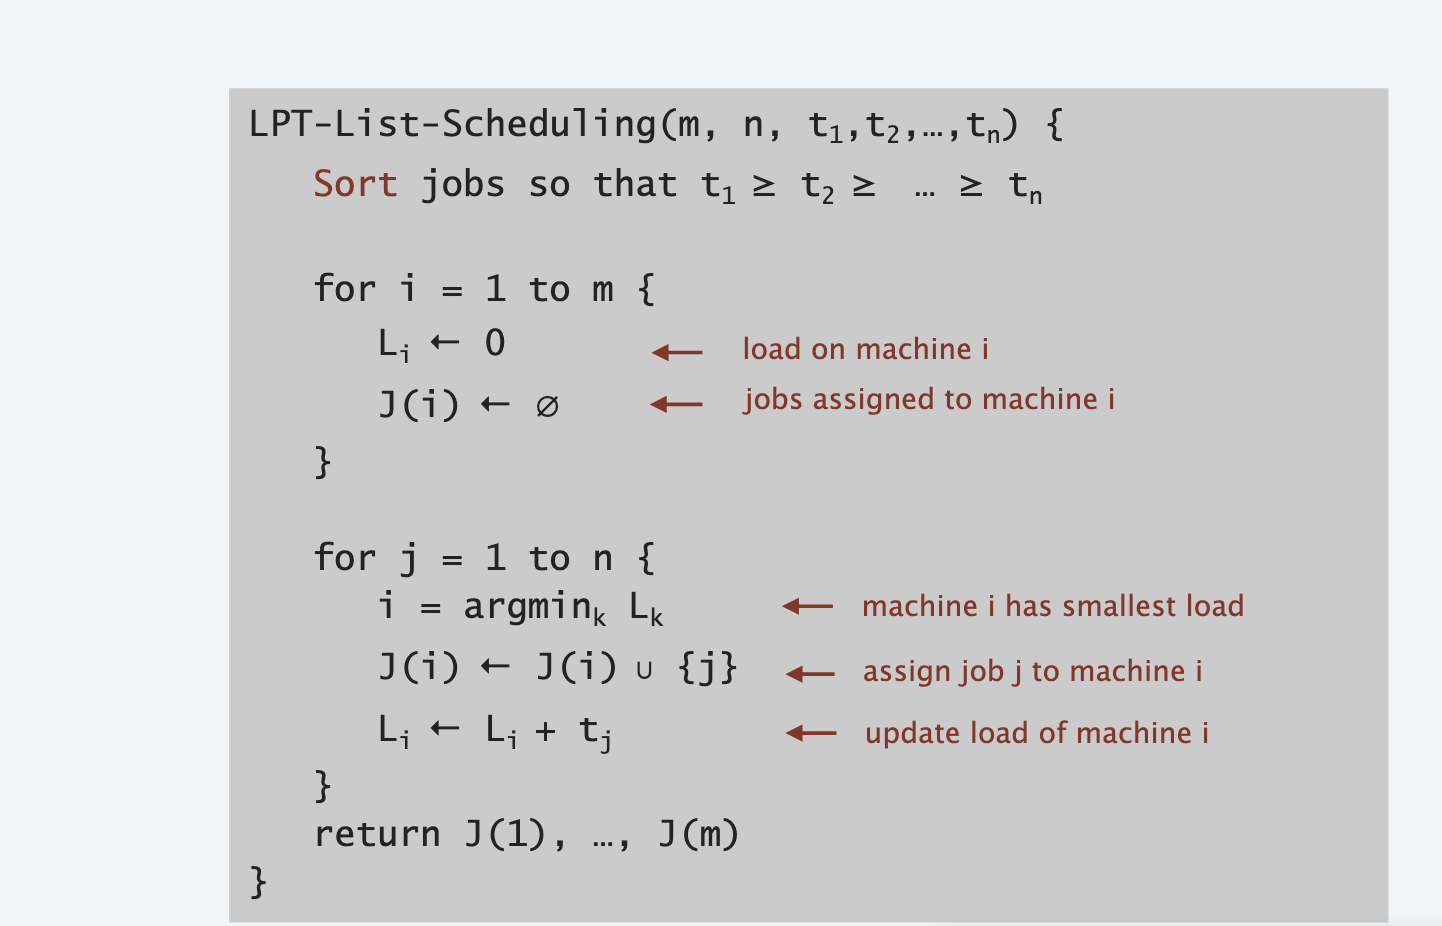
\includegraphics[width=1\textwidth]{imm/Screenshot 2026-05-15 alle 18.19.00.png}
\end{figure}

\textbf{Improvement idea:} Before running list scheduling, \textbf{sort the jobs from longest to shortest}. This prevents the worst case above (big job coming last).

\begin{theorem}{LPT is a $\frac{3}{2}$-Approximation}
    \newline
\textbf{Key extra lemma:} If there are more than $m$ jobs, then $L^* \geq 2t_{m+1}$.\\
\textit{Why?} The first $m+1$ jobs (in sorted order) are all at least as long as $t_{m+1}$. With $m+1$ jobs and $m$ machines, by the pigeonhole principle, at least one machine gets two of them. So $L^* \geq 2t_{m+1}$.

\textbf{Proof sketch:} Following the same logic as before, let $j$ be the last job on the bottleneck machine. After sorting, $j \geq m+1$ (it is not one of the first $m$ jobs), so:
\[
t_j \leq t_{m+1} \leq \frac{1}{2}L^*
\]
Therefore:
\[
L = (L_i - t_j) + t_j \leq L^* + \frac{1}{2}L^* = \frac{3}{2}L^*
\]
$\square$
\end{theorem}

%=============================================================
\section{Center Selection}
%=============================================================

\subsection{The Problem}

You have $n$ sites (think: towns) and you need to build $k$ facilities (think: hospitals). You want to place $k$ centers so that every site is \textbf{as close as possible} to some center.

Formally, the \textbf{covering radius} is:
\[
r(C) = \max_i \, dist(s_i, C) = \max_i \min_{c \in C} dist(s_i, c)
\]
\textbf{Goal:} Choose $k$ centers $C$ to minimise $r(C)$.
\begin{figure}[H]
    \centering
    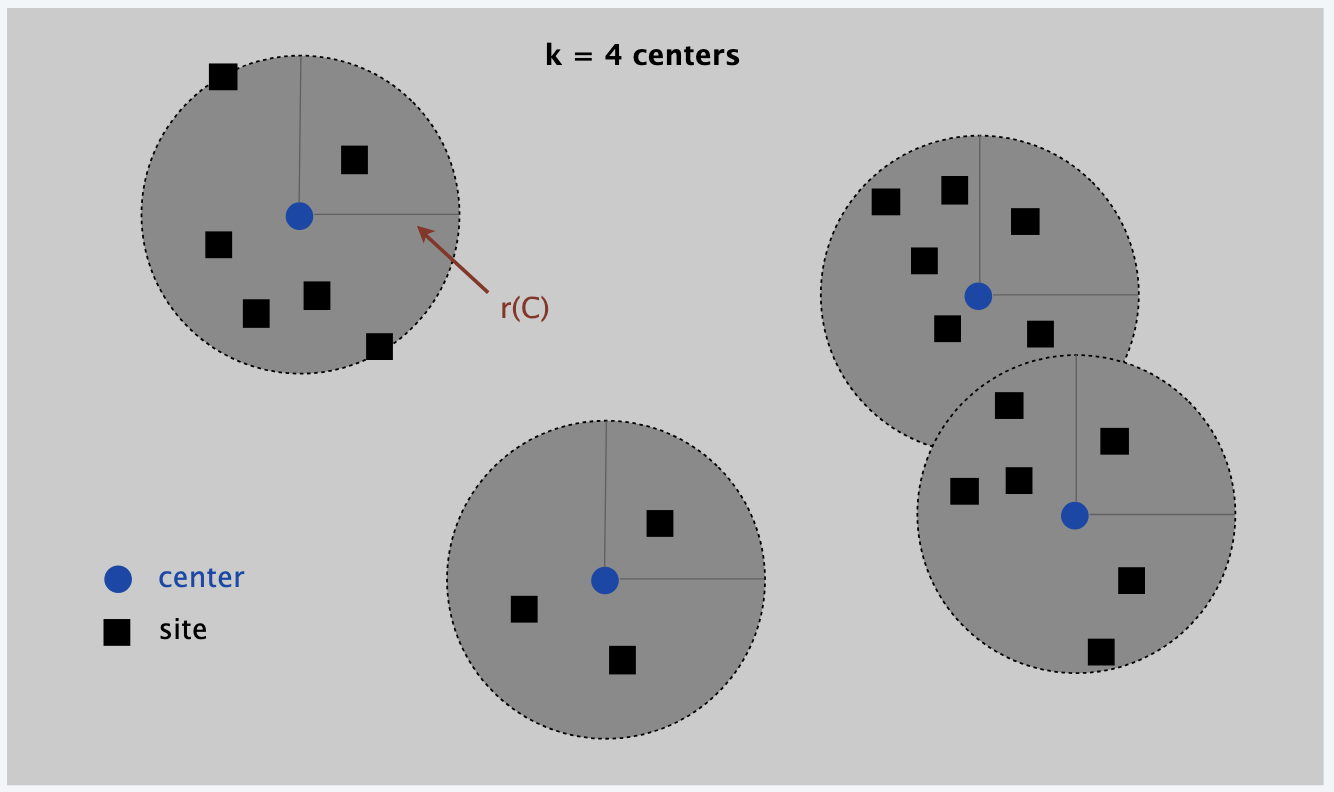
\includegraphics[width=0.5\textwidth]{imm/Screenshot 2026-05-15 alle 18.26.57.png}
    
\end{figure}

The distance satisfies three natural properties: $dist(x,x)=0$ (identity), $dist(x,y)=dist(y,x)$ (symmetry), and $dist(x,y) \leq dist(x,z)+dist(z,y)$ (triangle inequality).

\subsection{Wrong Greedy: A False Start}

\textbf{Bad idea:} Place the first center at the globally best single location, then greedily reduce the radius.\\
\textbf{Problem:} This can give an arbitrarily bad answer. The first center might ``attract'' both clusters, and the second center is placed far from where it is really needed.

\subsection{Correct Greedy Algorithm}

\textbf{Right idea:} Always place the next center at the \textbf{site farthest from any existing center}.

\begin{figure}[H]
    \centering
    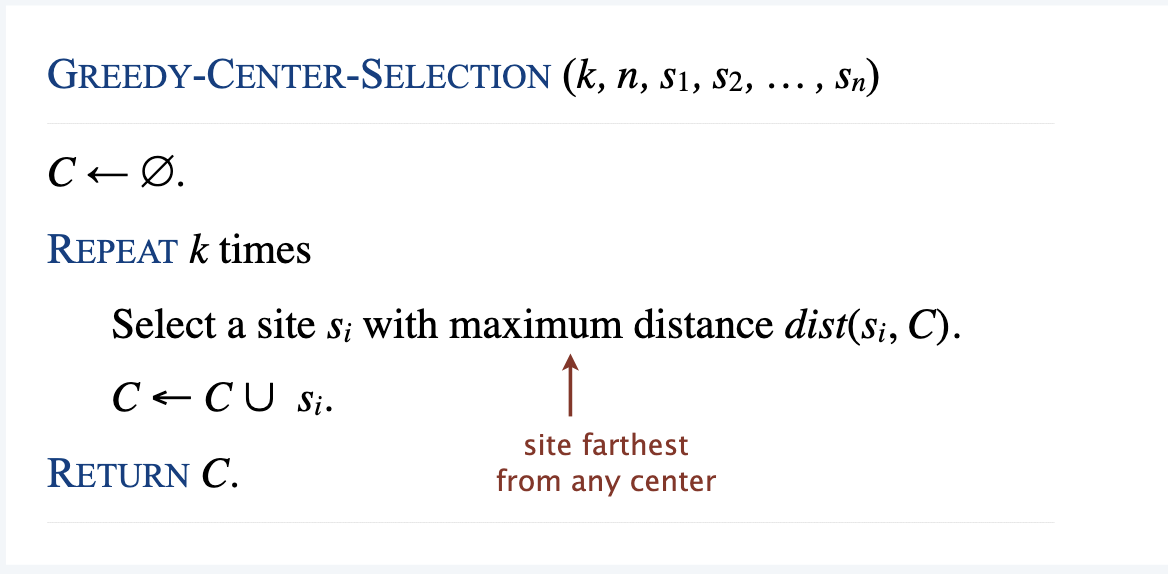
\includegraphics[width=1\textwidth]{imm/Screenshot 2026-05-15 alle 18.31.49.png}
\end{figure}

\textbf{Key property after termination:} All $k$ centers in $C$ are pairwise at distance $\geq r(C)$ from each other.\\
\textit{Why?} Because each new center was chosen as the farthest site at the time it was added. Once it is a center, no later center can be closer than $r(C)$ to it.

\begin{theorem}{Center Selection Greedy is a 2-Approximation}{}
Let $C^*$ be the optimal set of $k$ centers with radius $r^* = r(C^*)$.\\
Let $C$ be the greedy solution with radius $r = r(C)$.\\
Then $r \leq 2r^*$.

\textbf{Proof by contradiction:}\\
Assume $r^* < \frac{1}{2}r$, i.e., the optimal radius is less than half our radius.

\begin{enumerate}
    \item Draw a ball of radius $\frac{1}{2}r$ around each of our $k$ greedy centers $c_i \in C$.
    \item Our centers are all at distance $\geq r$ from each other, so these balls do not overlap.
    \item The optimal solution $C^*$ has $k$ centers. Since there are $k$ non-overlapping balls and $k$ optimal centers, by the pigeonhole principle, each ball contains exactly one optimal center $c_i^*$.
    \item Now take any site $s$. It has some closest optimal center $c_i^*$ at distance $\leq r^*$.\\
    By the triangle inequality:
    \[
    dist(s, c_i) \leq dist(s, c_i^*) + dist(c_i^*, c_i) \leq r^* + r^* = 2r^*
    \]
    (since both $s$ and $c_i$ are within $r^*$ of $c_i^*$, as the ball has radius $\frac{1}{2}r < r^*$... wait, let's be precise:)\\
    We assumed $r^* < \frac{1}{2}r$, so $dist(c_i^*, c_i) \leq \frac{1}{2}r < r^*$.\\
    Therefore $dist(s, c_i) \leq r^* + r^* = 2r^*$.
    \item This means $r(C) \leq 2r^*$, which \textbf{contradicts} our assumption. $\square$
\end{enumerate}
\end{theorem}

\textbf{Center selection in practice}{}
Sites: cities at positions 1, 5, 6, 10 on a line. $k=2$ centers.\\
\textbf{Greedy:} Start at city 1. Farthest site is city 10 $\to$ add it. Done: centers = $\{1, 10\}$.\\
Radius: worst site is 5 or 6. $dist(5, \{1,10\}) = \min(4, 5) = 4$. So $r = 4$.\\
\textbf{Optimal:} centers $= \{3.5, 8\}$ (non-sites!), giving radius $= 2.5$.\\
Note: the greedy is constrained to place centers \textit{on sites} yet gives $r = 4 \leq 2 \times 2.5 = 5$. The factor-2 bound holds.


\textbf{Is the 2-approximation the best possible?}\\
Yes (unless P = NP). A $(2-\varepsilon)$-approximation would let us solve DOMINATING-SET in polynomial time:
\begin{itemize}
    \item Build a CENTER-SELECTION instance from graph $G$: set $dist(u,v)=1$ if edge, $dist(u,v)=2$ if no edge.
    \item $G$ has a dominating set of size $k$ $\iff$ there are $k$ centers with radius $r^*=1$.
    \item A $(2-\varepsilon)$-approximation would find radius $r=1$ (since it cannot use edges of distance 2), solving DOMINATING-SET in poly-time.
\end{itemize}

%=============================================================
\section{Pricing Method: Vertex Cover}
%=============================================================

\subsection{Weighted Vertex Cover}

Recall that a \textbf{vertex cover} is a set of vertices $S$ such that every edge has at least one endpoint in $S$. Now each vertex $i$ has a weight $w_i \geq 0$, and we want the minimum total weight cover.

\textbf{Weighted Vertex Cover}{}
\begin{figure}[H]
    \centering
    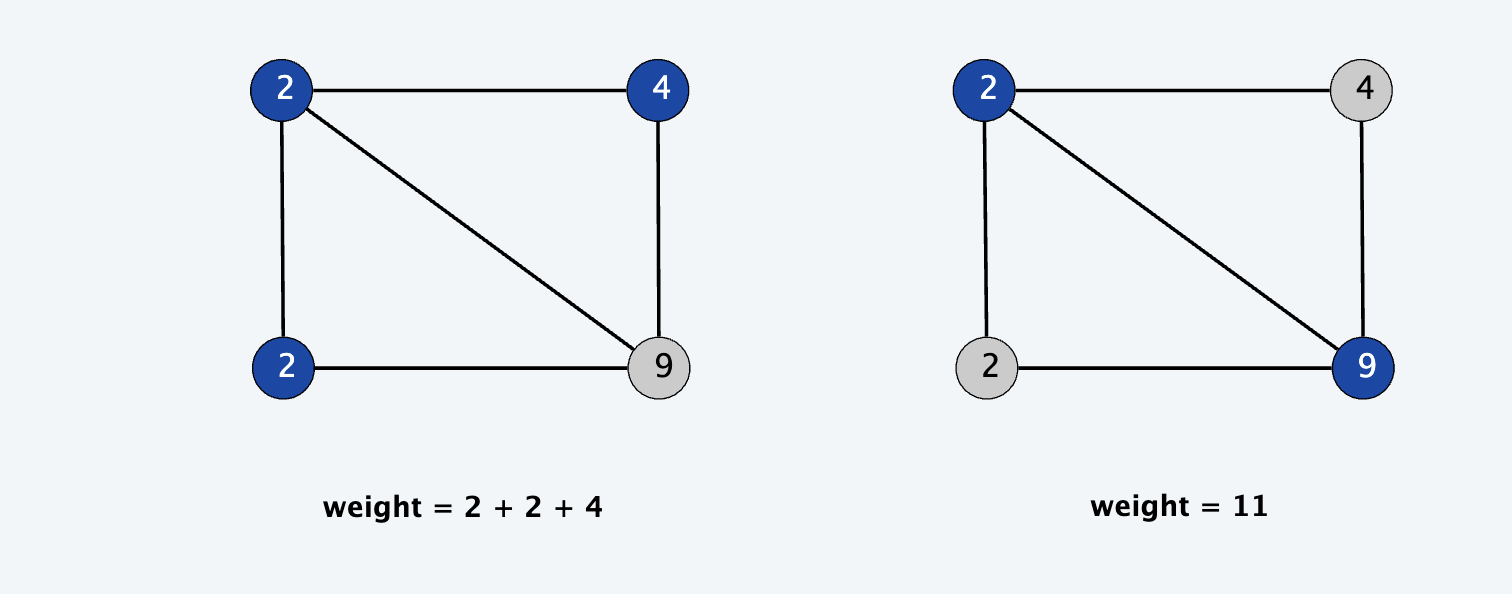
\includegraphics[width=0.5\textwidth]{imm/Screenshot 2026-05-15 alle 18.47.25.png}
\end{figure}
The pricing method will find an approximation of the minimum weight cover.


\subsection{The Pricing Idea}

Think of each edge as a \textbf{client} that must pay to use two vertices. Edge $e=(i,j)$ pays a price $p_e \geq 0$, and this price is split between vertex $i$ and vertex $j$.

\textbf{Fairness rule:} No vertex should be ``overcharged''. The total price paid by all edges incident to vertex $i$ must be $\leq w_i$:
\[
\sum_{e \ni i} p_e \leq w_i \quad \text{for all vertices } i
\]

A vertex is called \textbf{tight} when this inequality becomes an equality: all its ``budget'' $w_i$ is used up.

\begin{lemma}{Fairness Lemma}{}
For \textbf{any} vertex cover $S$ (not just ours) and \textbf{any} fair prices $p_e$:
\[
\sum_{e \in E} p_e \leq w(S) = \sum_{i \in S} w_i
\]
\textbf{Why?} Every edge in $E$ is covered by at least one vertex in $S$. So when we sum up $\sum_{i \in S} w_i$, each edge price $p_e$ is counted at least once. By fairness, $\sum_{e \ni i} p_e \leq w_i$ for each $i \in S$, so the total sum of prices is at most $w(S)$.

This lemma is powerful because it gives a lower bound on \textit{any} cover's cost: no matter how clever you are, the cover weight is at least $\sum_e p_e$.
\end{lemma}

\subsection{The Pricing Algorithm}

The idea is to increase edge prices gradually until we cannot do so without violating fairness, then collect all tight vertices.

\begin{verbatim}
Set all p_e = 0
S = empty set
While there exists an uncovered edge (i,j):
    Pick any uncovered edge e = (i,j)
    Raise p_e until vertex i or vertex j becomes tight
    (i.e., until sum of prices around i equals w_i, or around j equals w_j)
S = { all tight vertices }
Return S
\end{verbatim}

\textbf{Pricing Method Step by Step}{}
Graph with vertices $a$ (weight 4), $b$ (weight 2), $c$ (weight 6), edge $a$-$b$ and edge $b$-$c$.
\begin{itemize}
    \item Edge $a$-$b$ is uncovered. Raise $p_{ab}$ from 0.\\
    $b$ becomes tight when $p_{ab} = 2$ (since $w_b = 2$). So set $p_{ab} = 2$.
    \item Now vertex $b$ is tight and is in $S$.
    \item Edge $b$-$c$ is covered by $b$ (which is now in $S$). No more uncovered edges.
    \item $S = \{b\}$, but wait --- $a$ is not in $S$, so edge $a$-$b$ is covered only by $b$. Check: $b \in S$ covers $a$-$b$, and $b \in S$ covers $b$-$c$. \checkmark
    \item Total weight $w(S) = w_b = 2$.
    \item Total prices $\sum_e p_e = p_{ab} = 2$.
    \item $w(S) = 2 \leq 2 \cdot 2 = 4 \leq 2 w(S^*)$. \checkmark
\end{itemize}

\begin{theorem}{Pricing Method is a 2-Approximation}{}
Let $S$ be the set returned by the pricing algorithm and $S^*$ be any optimal cover. Then:
\[
w(S) \leq 2\,w(S^*)
\]

\textbf{Proof:}

\textbf{Step 1 --- $S$ is a valid vertex cover.}\\
Every tight vertex is in $S$. If some edge $(i,j)$ were not covered, then neither $i$ nor $j$ would be tight. But then the while loop would keep running and raise $p_{(i,j)}$ until one becomes tight. Contradiction: the loop would not have stopped. So all edges are covered.

\textbf{Step 2 --- The approximation bound.}\\
Every vertex in $S$ is tight, so $w_i = \sum_{e \ni i} p_e$ for all $i \in S$. Therefore:
\[
w(S) = \sum_{i \in S} w_i = \sum_{i \in S} \sum_{e \ni i} p_e
\]
Now extend the sum to all vertices in $V$ (this only makes it larger, since prices are $\geq 0$):
\[
\sum_{i \in S} \sum_{e \ni i} p_e \leq \sum_{i \in V} \sum_{e \ni i} p_e = 2\sum_{e \in E} p_e
\]
The last equality holds because each edge $(i,j)$ appears \textbf{exactly twice} in the double sum: once when $i$ is the vertex, and once when $j$ is.

By the Fairness Lemma, $\sum_{e \in E} p_e \leq w(S^*)$. Combining:
\[
w(S) \leq 2\sum_{e \in E} p_e \leq 2\,w(S^*) \qquad \square
\]
\end{theorem}





\end{document}